% Informe del TP final de Machine Learning — Maestría en IA, Universidad de Palermo
% Compilar en Overleaf con pdfLaTeX + Biber (Menu > Settings > Compiler: pdfLaTeX).
\documentclass[11pt,a4paper,oneside]{report}

\usepackage[utf8]{inputenc}
\usepackage[T1]{fontenc}
\usepackage[spanish,es-tabla,es-nodecimaldot,es-noshorthands]{babel}
\usepackage{lmodern}
\usepackage{microtype}
\usepackage[margin=2.5cm]{geometry}
\usepackage{amsmath,amssymb,amsthm,mathtools,bm}
\usepackage{dsfont}  % \mathds{1}: función indicadora
\usepackage{graphicx}
\usepackage{booktabs,tabularx,multirow}
\usepackage{siunitx}
\sisetup{output-decimal-marker={,}, group-separator={.}, group-minimum-digits=4}
\usepackage{caption,subcaption}
\usepackage{xcolor}
\usepackage{algorithm,algpseudocode}
\usepackage{tikz}
\floatname{algorithm}{Algoritmo}
\renewcommand{\listalgorithmname}{Lista de algoritmos}
\algrenewcommand\algorithmicrequire{\textbf{Entrada:}}
\algrenewcommand\algorithmicensure{\textbf{Salida:}}
\algrenewcommand\algorithmicfor{\textbf{para}}
\algrenewcommand\algorithmicdo{\textbf{hacer}}
\algrenewcommand\algorithmicwhile{\textbf{mientras}}
\algrenewcommand\algorithmicif{\textbf{si}}
\algrenewcommand\algorithmicthen{\textbf{entonces}}
\algrenewcommand\algorithmicelse{\textbf{si no}}
\algrenewcommand\algorithmicend{\textbf{fin}}
\algrenewcommand\algorithmicreturn{\textbf{devolver}}
\algrenewcommand\algorithmicloop{\textbf{repetir}}
\usepackage[backend=biber,style=authoryear,maxcitenames=2,uniquelist=false]{biblatex}
\addbibresource{referencias.bib}
\usepackage[hidelinks]{hyperref}
\usepackage[nameinlink,noabbrev,spanish]{cleveref}

\graphicspath{{figuras/}}

\theoremstyle{definition}
\newtheorem{definicion}{Definición}[chapter]
\theoremstyle{plain}
\newtheorem{teorema}{Teorema}[chapter]
\newtheorem{proposicion}[teorema]{Proposición}
\newtheorem{lema}[teorema]{Lema}
\theoremstyle{remark}
\newtheorem{observacion}{Observación}[chapter]

\newcommand{\R}{\mathbb{R}}
\newcommand{\E}{\mathbb{E}}
\newcommand{\vx}{\mathbf{x}}
\newcommand{\vw}{\mathbf{w}}
\newcommand{\vth}{\boldsymbol{\theta}}
\DeclareMathOperator*{\argmax}{arg\,max}
\DeclareMathOperator*{\argmin}{arg\,min}

\title{Detección automática de crisis epilépticas en EEG:\\
fundamentos matemáticos, modelos convexos, redes convolucionales\\
y comparativa de optimizadores}
\author{Vicente Matias Danguise\\[2mm]
Maestría en Inteligencia Artificial — Universidad de Palermo\\
Machine Learning — Trabajo final individual}
\date{Noviembre de 2026}

\begin{document}
\maketitle

\begin{abstract}
Este trabajo estudia la detección automática de crisis epilépticas en el electroencefalograma (EEG) con dos bases
públicas: Bonn (500 segmentos de un canal) y CHB-MIT (6 pacientes, 223 horas de registro continuo de 18 canales y 34
crisis, que ocupan el 0,37~\% del tiempo). Cada paso tiene su fundamento matemático. A partir de un modelo de la señal
con y sin crisis se deducen los atributos (potencia por banda con la transformada de Fourier y el método de Welch) y una
calibración por paciente, que consiste en restar la mediana de cada atributo. Se desarrollan la optimalidad local y global
y la convexidad, la convergencia del descenso por gradiente, los multiplicadores de Lagrange y las condiciones KKT, el
método simplex y el lema de Neyman-Pearson, que da el umbral de decisión con una tasa de falsas alarmas fija.

En Bonn, con 20 atributos espectrales, la regresión logística alcanza 97,4~\% de exactitud en tres clases y el SVM con núcleo
RBF, 98,4~\%. Se verifica numéricamente que en la logística, que es convexa, 20 puntos iniciales llegan al mismo óptimo, y que
una red neuronal chica termina en 8 mínimos distintos. En CHB-MIT, evaluando sobre un paciente no visto, la logística
calibrada detecta 24 de 34 crisis con 1,1 falsas alarmas por hora.

Una red convolucional sobre espectrogramas se entrena con seis optimizadores (SGD, Momentum, Nesterov, RMSprop, Adam y
AdamW), tres tasas de aprendizaje y cinco semillas. Con la tasa elegida por validación, SGD es significativamente mejor
(AUC de prueba $0{,}976 \pm 0{,}006$). Pero un experimento exploratorio muestra que con la tasa alta SGD, RMSprop, Adam y AdamW
quedan empatados: pesa más la tasa que el algoritmo. El paciente de validación quedó saturado y no sirvió para elegir. En los
pacientes de prueba, la red detecta 10 de 14 crisis con 0,19 falsas alarmas por hora, contra 6 de 14 con 0,54 de la regresión
logística, a pesar de tener menor AUC. Para un detector de crisis, la métrica relevante es la sensibilidad con muy pocas falsas
alarmas, no el AUC.

\medskip
\noindent\textbf{Palabras clave:} epilepsia, EEG, transformada de Fourier, convexidad, multiplicadores de Lagrange,
Neyman-Pearson, redes convolucionales, optimizadores.

\end{abstract}

\tableofcontents
\listoffigures
\listoftables

\chapter{Introducción}
\label{cap:introduccion}

\section{Motivación}

La epilepsia es una de las enfermedades neurológicas crónicas más frecuentes: afecta a unos 50 millones de personas en
el mundo \parencite{who2024}. Clínicamente se define por una predisposición duradera a generar crisis epilépticas no
provocadas; en la práctica, por dos crisis no provocadas separadas por más de 24 horas, o una crisis con un riesgo de
recurrencia alto \parencite{fisher2014}. Una \emph{crisis} es un episodio transitorio de actividad neuronal anormalmente
excesiva o sincrónica. Esa sincronía es la que hace que la crisis sea visible en el electroencefalograma (EEG): millones
de neuronas que descargan juntas producen oscilaciones de gran amplitud y frecuencia definida, muy distintas de la
actividad de fondo.

El EEG es la herramienta central para diagnosticar la epilepsia, clasificar el tipo de crisis y decidir el tratamiento.
En una unidad de monitoreo se registran pacientes durante días seguidos, con decenas de canales, para capturar sus crisis.
Revisar a mano ese volumen es lento y caro: un registro de 24 horas lleva horas de lectura de un especialista, y las
crisis ocupan una fracción mínima del tiempo (el 0,37~\% en los datos de este trabajo). Un \textbf{detector automático}
que marque los momentos sospechosos sirve para dos cosas: acortar la revisión y avisar al personal mientras la crisis
ocurre, cuando todavía se puede intervenir.

La dificultad no es separar una crisis típica de la actividad normal, que un modelo simple hace bien, sino hacerlo
\emph{con muy pocas falsas alarmas} y \emph{en un paciente que el modelo no vio}. Con 900 ventanas de 4~s por hora, una
especificidad de 99~\% da 9 falsas alarmas por hora, inaceptables en la práctica. Y el EEG de cada persona es distinto:
cambian la amplitud, las frecuencias dominantes y la forma de las crisis. Estas dos condiciones (desbalance extremo y
variabilidad entre pacientes) atraviesan todo el trabajo y son las que determinan las métricas, los modelos y las
conclusiones.

\section{El problema como aprendizaje automático}

Formalmente, el EEG de un paciente se divide en ventanas de duración fija y a cada ventana $\mathbf{X}$ se le asigna una
etiqueta $y \in \{0, 1\}$ (crisis o no). El objetivo es aprender una función $s(\mathbf{X})$, un \emph{puntaje}, tal que
la regla $\hat y = \mathds{1}[s(\mathbf{X}) > \tau]$ detecte la mayor cantidad de crisis con una tasa de falsas alarmas
acotada. Eso conecta el problema con cuatro áreas que el trabajo desarrolla:
\begin{itemize}
  \item \textbf{Procesamiento de señales.} La crisis se manifiesta como un cambio en el contenido de frecuencias. La
        transformada de Fourier y sus estimadores (periodograma, Welch, espectrograma) convierten la señal en atributos
        que hacen visible ese cambio.
  \item \textbf{Optimización.} Entrenar un modelo es minimizar una función de pérdida. Si es convexa (regresión logística,
        SVM), todo mínimo local es global y el resultado no depende del punto inicial. Si no lo es (redes neuronales), sí,
        y la elección del algoritmo y de su tasa de aprendizaje pasa a ser parte del modelo.
  \item \textbf{Optimización con restricciones.} El umbral $\tau$ no se elige minimizando el error: se elige maximizando la
        sensibilidad con una tasa de falsos positivos fija. Es un problema con restricción, que se resuelve con un
        multiplicador de Lagrange (lema de Neyman-Pearson) y, en su versión discreta, con programación lineal.
  \item \textbf{Evaluación.} Exactitud, sensibilidad, especificidad, curva ROC, AUC y matriz de confusión miden cosas
        distintas, y con clases tan desbalanceadas algunas pueden ser engañosas. A esas se suman las métricas clínicas:
        crisis detectadas, falsas alarmas por hora y latencia.
\end{itemize}

\section{Objetivos}

\begin{enumerate}
  \item Formular la detección de crisis como un problema de procesamiento de señales y de clasificación, a partir de un
        modelo matemático del fenómeno.
  \item Fundamentar matemáticamente cada paso: transformada de Fourier, convexidad y optimalidad local y global,
        multiplicadores de Lagrange y condiciones KKT, método simplex y umbral de Neyman-Pearson.
  \item Verificar numéricamente esos resultados sobre datos reales: unicidad del óptimo en un problema convexo, mínimos
        múltiples en uno no convexo, condiciones KKT en el dual del SVM.
  \item Entrenar y evaluar modelos convexos (regresión logística, SVM) y una red convolucional sobre espectrogramas.
  \item Comparar seis optimizadores de primer orden (SGD, Momentum, Nesterov, RMSprop, Adam, AdamW) sobre la misma red, con
        varias semillas y pruebas estadísticas.
  \item Evaluar con métricas clínicas: sensibilidad y especificidad por ventana, sensibilidad por evento, falsas alarmas
        por hora y latencia, sobre pacientes que no se usaron para entrenar.
\end{enumerate}

\section{Datos}

Se usan dos bases públicas, descargadas de sus fuentes oficiales:
\begin{itemize}
  \item \textbf{Bonn} \parencite{andrzejak2001}: 500 segmentos de 23,6~s de un canal, en cinco grupos (voluntarios sanos,
        pacientes fuera de crisis y pacientes durante crisis). Es chica, limpia y balanceada; sirve para estudiar el
        espectro de las crisis y para ilustrar la teoría con un problema de tres clases.
  \item \textbf{CHB-MIT} \parencite{shoeb2009,goldberger2000}: registros continuos de 23 canales de niños con epilepsia
        refractaria. Se usan 6 pacientes, 223 horas y 34 crisis. Tiene el desbalance real y permite evaluar en pacientes
        nuevos.
\end{itemize}

\section{Contribuciones}

Más allá de reproducir técnicas conocidas, el trabajo llega a algunos resultados que no eran evidentes al principio:
\begin{itemize}
  \item Una \textbf{calibración por paciente} muy simple, restar la mediana de cada atributo, se deduce del modelo
        multiplicativo del EEG y sube el AUC de la regresión logística de 0,80 a 0,93 en pacientes nuevos.
  \item En la comparativa de optimizadores, \textbf{la ventaja de SGD sobre los métodos adaptativos resultó ser un efecto de la
        tasa de aprendizaje}: con la tasa alta de cada grilla, SGD, RMSprop, Adam y AdamW quedan empatados.
  \item \textbf{Un solo paciente de validación no sirve para elegir hiperparámetros}: está saturado (AUC entre 0,996 y 0,999
        para todas las redes) y no predice el desempeño en prueba.
  \item \textbf{El modelo con menor AUC es el mejor detector}: la red convolucional tiene menor AUC que la regresión logística
        calibrada, pero detecta 11 de 14 crisis contra 7, con las mismas falsas alarmas y la mitad de latencia. La
        diferencia está en la zona de pocas falsas alarmas, que el AUC no pondera.
\end{itemize}

\section{Organización del trabajo}

\begin{itemize}
  \item El \textbf{Capítulo~\ref{cap:fenomeno}} describe el fenómeno: el origen fisiológico del EEG, un modelo matemático de
        la señal con y sin crisis, y las hipótesis que se ponen a prueba.
  \item El \textbf{Capítulo~\ref{cap:fourier}} desarrolla la transformada de Fourier discreta, el muestreo, el filtrado y la
        estimación espectral (periodograma, Welch, espectrograma), aplicados a Bonn.
  \item El \textbf{Capítulo~\ref{cap:datos}} presenta las dos bases, el preprocesamiento, el análisis exploratorio, las
        particiones y la calibración por paciente.
  \item El \textbf{Capítulo~\ref{cap:metricas}} define las métricas: matriz de confusión, sensibilidad, especificidad, curva ROC
        y AUC, métricas por evento, el umbral de Neyman-Pearson y los esquemas de validación y pruebas estadísticas.
  \item El \textbf{Capítulo~\ref{cap:optimizacion}} es el núcleo teórico: optimalidad local y global, convexidad, descenso por
        gradiente y su convergencia, multiplicadores de Lagrange y KKT, el método simplex, el dual del SVM y el lema de
        Neyman-Pearson.
  \item El \textbf{Capítulo~\ref{cap:convexos}} entrena regresión logística y SVM en Bonn y en CHB-MIT, verifica numéricamente la
        teoría y evalúa en pacientes nuevos con validación dejando un paciente afuera.
  \item El \textbf{Capítulo~\ref{cap:cnn}} describe la red convolucional, la retropropagación, los seis optimizadores con su
        análisis y el diseño del experimento.
  \item El \textbf{Capítulo~\ref{cap:resultados}} presenta la comparativa de optimizadores, la evaluación clínica de la red y su
        comparación con los modelos convexos.
  \item El \textbf{Capítulo~\ref{cap:conclusiones}} discute los resultados, las limitaciones y el trabajo futuro.
  \item El \textbf{Apéndice~\ref{ap:reproducibilidad}} explica cómo reproducir todos los resultados.
\end{itemize}

\section{Reproducibilidad}

Todo el código es propio y está en Python: cuatro notebooks, uno por etapa del trabajo, y cuatro scripts para la descarga,
el preprocesamiento, las métricas y el entrenamiento de la red. Cada tabla y cada figura del informe sale de un archivo
generado por esos notebooks. Las versiones de las bibliotecas y los pasos para reproducir están en el
Apéndice~\ref{ap:reproducibilidad}. Todo se corrió en una computadora personal sin GPU.

\chapter{El fenómeno: EEG y crisis epilépticas}
\label{cap:fenomeno}

Este capítulo describe qué se mide, por qué una crisis deja una huella en la señal y cómo se traduce
esa huella en un modelo matemático. El modelo de la ecuación~\eqref{eq:modelo_eeg} es la base de todo
lo que sigue: justifica el uso de la transformada de Fourier (Capítulo~\ref{cap:fourier}), los atributos de
potencia por banda, la calibración por paciente y el planteo de la detección como un test de hipótesis.

\section{Epilepsia y crisis}

Una \emph{crisis epiléptica} es la aparición transitoria de signos o síntomas debidos a una actividad
neuronal anormalmente excesiva o sincrónica en el cerebro. La \emph{epilepsia} es la enfermedad que
predispone a sufrir crisis en forma recurrente; en la práctica clínica se diagnostica, entre otros
criterios, tras dos crisis no provocadas separadas por más de 24 horas \parencite{fisher2014}.

Para el diagnóstico y el ajuste del tratamiento se registra el electroencefalograma (EEG) durante
horas o días. Las crisis ocupan una fracción muy chica de ese tiempo: en los seis pacientes de
CHB-MIT usados en este trabajo, 34 crisis suman el 0,37~\% de 222,8 horas de registro. Revisar todo
el registro a mano es lento, y esa es la motivación de la detección automática.

\section{Origen de la señal de EEG}

El EEG mide diferencias de potencial eléctrico generadas por la actividad del cerebro. La mayor
parte de la señal proviene de las corrientes postsinápticas de las neuronas piramidales de la corteza.
Estas neuronas están alineadas en forma perpendicular a la superficie cortical, de modo que cuando
miles de ellas reciben entradas sincronizadas sus corrientes se suman y el conjunto se comporta como
un \emph{dipolo} de corriente. Un potencial de acción aislado es demasiado breve y local para verse en
la superficie; lo que se registra es la suma de actividad lenta y sincronizada de millones de neuronas.

El potencial que genera ese dipolo atraviesa el líquido cefalorraquídeo, el cráneo y el cuero
cabelludo, que actúan como un conductor de volumen: atenúan la señal y la difunden espacialmente.
Por eso la amplitud típica del EEG de superficie es de decenas de microvoltios, mientras que el EEG
intracraneal (electrodos sobre la corteza o dentro de ella, como en los sets C, D y E de Bonn) alcanza
cientos.

La consecuencia importante para el modelado es que la amplitud registrada depende mucho de la
\emph{sincronía}: $M$ fuentes con fases aleatorias producen una amplitud que crece como $\sqrt{M}$,
mientras que $M$ fuentes en fase producen una amplitud que crece como $M$. Una crisis, que es por
definición actividad excesivamente sincrónica, se ve como un aumento grande de amplitud.

\section{Ritmos y bandas de frecuencia}

El EEG normal no es ruido blanco: tiene oscilaciones características (ritmos) que se describen por su
banda de frecuencia (Tabla~\ref{tab:bandas}).

\begin{table}[ht]
\centering
\caption{Bandas de frecuencia clásicas del EEG, con los límites usados en este trabajo.}
\label{tab:bandas}
\begin{tabular}{llp{8cm}}
\toprule
Banda & Rango [Hz] & Contexto típico \\
\midrule
delta $\delta$ & 0,5--4 & sueño profundo; actividad lenta patológica en vigilia \\
theta $\theta$ & 4--8 & somnolencia; frecuente en descargas ictales \\
alfa $\alpha$ & 8--13 & vigilia relajada con ojos cerrados, en zonas occipitales \\
beta $\beta$ & 13--30 & vigilia activa, concentración \\
gamma $\gamma$ & 30--40 & actividad rápida (acotada a 40 Hz por el filtro) \\
\bottomrule
\end{tabular}
\end{table}

Un ejemplo de los datos: en Bonn, el set B (voluntarios sanos, ojos cerrados) tiene el 47,6~\% de su
potencia en la banda alfa, contra el 24,1~\% del set A (los mismos voluntarios con los ojos abiertos).
Es el ritmo alfa occipital, que se atenúa al abrir los ojos (Capítulo~\ref{cap:fourier}).

\section{Qué cambia durante una crisis}

Durante una crisis aparece una \emph{descarga rítmica}: una oscilación de gran amplitud, casi
periódica, que puede empezar en una zona (crisis focal) y propagarse, o comprometer los dos hemisferios
desde el inicio (crisis generalizada). En los datos de este trabajo se observa que:

\begin{itemize}
  \item En Bonn, los segmentos ictales (set E) tienen un desvío estándar de 341~µV contra 48--90~µV
        de los demás sets, y entre 10 y 100 veces más potencia entre 3 y 25 Hz.
  \item En CHB-MIT la potencia media sube en \emph{todas} las bandas y en \emph{todos} los pacientes, entre 2 y
        50 veces; pero la banda que más sube depende del paciente: delta en chb01 y chb08, alfa y
        beta en chb05 y chb10 (Capítulo~\ref{cap:datos}).
  \item Después de la crisis queda un período de actividad lenta de gran amplitud (estado
        \emph{post-ictal}) que no se anota como crisis.
\end{itemize}

\section{Modelo matemático de la señal}
\label{sec:modelo}

\subsection{Montaje bipolar}

Cada electrodo $e$ registra un potencial $v_e(t)$ respecto de una referencia. En el montaje bipolar de
CHB-MIT, cada canal es la diferencia entre dos electrodos vecinos del sistema 10-20:
\begin{equation}
  x_{A\text{-}B}(t) = v_A(t) - v_B(t).
  \label{eq:bipolar}
\end{equation}
La resta cancela lo que es común a los dos electrodos (la referencia, buena parte de la interferencia
de red y de la actividad lejana) y resalta la actividad local entre ellos. Se usan los 18 canales de la
``doble banana''; en adelante $x_c(t)$, $c = 1,\dots,C$, denota el canal $c$.

\subsection{Modelo aditivo}

Se modela la señal registrada en el canal $c$ como la suma de cuatro componentes:
\begin{equation}
\boxed{\;
  x_c(t) \;=\; g_{p,c}\Big[\, \underbrace{b_c(t)}_{\text{fondo}}
  \;+\; \underbrace{\mathds{1}_{\mathcal{C}}(t)\, s_c(t)}_{\text{descarga ictal}} \,\Big]
  \;+\; \underbrace{a_c(t)}_{\text{artefactos}}
  \;+\; \underbrace{\eta_c(t)}_{\text{ruido}}
\;}
\label{eq:modelo_eeg}
\end{equation}
donde:
\begin{itemize}
  \item $b_c(t)$ es la \textbf{actividad de fondo}, modelada como una suma de osciladores en las bandas
        de la Tabla~\ref{tab:bandas} con amplitudes y fases que varían lentamente:
        \begin{equation}
          b_c(t) = \sum_{k} A_{c,k}(t) \cos\!\big(2\pi f_k t + \varphi_{c,k}(t)\big).
          \label{eq:fondo}
        \end{equation}
        En ventanas de pocos segundos se la trata como un proceso estacionario de media cero con densidad
        espectral $S_{b,c}(f)$.
  \item $\mathcal{C} = \bigcup_j [a_j, b_j]$ es el conjunto de intervalos con crisis, y
        $\mathds{1}_{\mathcal{C}}(t)$ vale 1 dentro de una crisis y 0 fuera.
  \item $s_c(t)$ es la \textbf{descarga ictal}, una oscilación casi periódica con frecuencia fundamental
        $f_0(t)$ (típicamente entre 3 y 8 Hz, que puede variar a lo largo de la crisis) y armónicos:
        \begin{equation}
          s_c(t) = \sum_{h=1}^{H} B_{c,h}(t) \cos\!\big(2\pi h\, f_0(t)\, t + \psi_{c,h}\big).
          \label{eq:descarga}
        \end{equation}
        Las amplitudes $B_{c,h}$ son grandes en los canales cercanos al foco y pueden ser casi nulas en los
        demás.
  \item $g_{p,c} > 0$ es una \textbf{ganancia} que depende del paciente $p$ y del canal: espesor del cráneo,
        impedancia de los electrodos, edad. Es la que hace que el ``nivel basal'' sea distinto entre
        pacientes.
  \item $a_c(t)$ son \textbf{artefactos} (movimiento, músculo, parpadeo, electrodo suelto) y $\eta_c(t)$ es
        ruido del equipo e interferencia de banda angosta (50 Hz en Bonn; 16 y 32 Hz en algunos registros
        de CHB-MIT).
\end{itemize}

\subsection{Consecuencia en el dominio de la frecuencia}

Si las componentes son procesos independientes y de media cero, sus densidades espectrales se
suman (el espectro de una suma de procesos no correlacionados es la suma de los espectros):
\begin{equation}
  S_{x_c}(f) = g_{p,c}^2 \Big[ S_{b,c}(f) + \mathds{1}_{\mathcal{C}}\, S_{s,c}(f) \Big] + S_{a,c}(f) + S_{\eta,c}(f).
  \label{eq:espectro_modelo}
\end{equation}
La potencia en una banda $\mathcal{B} = [f_1, f_2)$ es la integral de la densidad espectral,
$P_{c,\mathcal{B}} = \int_{\mathcal{B}} S_{x_c}(f)\,df$. Ignorando artefactos y ruido, el cociente entre la potencia
durante y fuera de la crisis es
\begin{equation}
  \frac{P^{\text{crisis}}_{c,\mathcal{B}}}{P^{\text{basal}}_{c,\mathcal{B}}}
  = 1 + \frac{\int_{\mathcal{B}} S_{s,c}(f)\,df}{\int_{\mathcal{B}} S_{b,c}(f)\,df} \;>\; 1,
\end{equation}
y en escala logarítmica
\begin{equation}
  \log_{10} P^{\text{crisis}}_{c,\mathcal{B}} - \log_{10} P^{\text{basal}}_{c,\mathcal{B}}
  = \log_{10}\!\left(1 + \frac{P_{s,c,\mathcal{B}}}{P_{b,c,\mathcal{B}}}\right) > 0.
  \label{eq:dif_log}
\end{equation}
Tres consecuencias directas del modelo:
\begin{enumerate}
  \item \textbf{La potencia por banda es un buen atributo.} La crisis suma potencia, sobre todo en las
        bandas que contienen $f_0$ y sus armónicos. Por eso la transformada de Fourier es la herramienta
        natural (Capítulo~\ref{cap:fourier}).
  \item \textbf{El logaritmo convierte la ganancia en una constante aditiva.} Como
        $\log P_{c,\mathcal{B}} = 2\log g_{p,c} + \log\!\big(P_{b,c,\mathcal{B}} + \mathds{1}_{\mathcal{C}}P_{s,c,\mathcal{B}}\big)$,
        el término $2\log g_{p,c}$ no depende del tiempo ni de la clase. Restar la mediana de cada
        paciente (que, al ser las crisis menos del 1~\% del tiempo, es esencialmente el nivel basal) lo
        elimina. Esta es la justificación de la \emph{calibración por paciente} que se usa en los
        Capítulos~\ref{cap:convexos} y~\ref{cap:cnn}.
  \item \textbf{La banda que más cambia depende de $f_0$ y de $S_{b,c}$}, que varían entre pacientes. Un
        detector que funcione para pacientes nuevos tiene que combinar varias bandas y canales.
\end{enumerate}

\section{La detección como test de hipótesis}
\label{sec:hipotesis}

Se divide la señal en ventanas de $L = 4$ s. Para cada ventana $w$, con sus datos $\mathbf{X}_w$ (los
18 canales), hay dos hipótesis:
\begin{equation}
  H_0:\ \mathbf{X}_w = \text{fondo} + \text{artefactos} + \text{ruido} \qquad\text{(sin crisis)},
  \qquad
  H_1:\ \mathbf{X}_w \text{ incluye además } s_c(t) \qquad\text{(crisis)}.
\end{equation}
Un detector calcula un puntaje $s(\mathbf{x})$ a partir de los atributos $\mathbf{x}$ de la ventana y
decide $H_1$ si $s(\mathbf{x}) > \tau$. El lema de Neyman-Pearson (Sección~\ref{sec:neyman_pearson})
dice que el mejor puntaje posible es la razón de verosimilitud $p(\mathbf{x}\mid H_1)/p(\mathbf{x}\mid H_0)$.
Como esas densidades son desconocidas, se aproximan con modelos entrenados con datos: regresión logística,
SVM y una red convolucional.

\paragraph{El problema del desbalance.} Con probabilidad a priori de crisis $\pi_1 \approx 0{,}0037$,
la regla de Bayes dice que la probabilidad de crisis dada una ventana es
\begin{equation}
  P(H_1 \mid \mathbf{x}) = \frac{\pi_1\, p(\mathbf{x}\mid H_1)}{\pi_1\, p(\mathbf{x}\mid H_1) + \pi_0\, p(\mathbf{x}\mid H_0)}.
\end{equation}
Para que esta probabilidad supere 1/2 hace falta que la razón de verosimilitud supere
$\pi_0/\pi_1 \approx 270$. Un clasificador que nunca detecta nada acierta el 99,6~\% de las ventanas; por
eso la exactitud (\emph{accuracy}) no sirve como métrica y en el Capítulo~\ref{cap:metricas} se usan
sensibilidad, especificidad, falsas alarmas por hora y curvas ROC.

\chapter{Procesamiento de señales y transformada de Fourier}
\label{cap:fourier}

El modelo del Capítulo~\ref{cap:fenomeno} dice que una crisis agrega potencia en ciertas frecuencias. Para
medirla hay que pasar la señal del dominio del tiempo al de la frecuencia. Este capítulo presenta la
transformada de Fourier en sus versiones continua y discreta, los problemas que aparecen al estimar
un espectro con una señal finita y muestreada (fuga espectral, varianza), y las soluciones que se usan
en el trabajo: ventanas de Hann, método de Welch, filtrado digital y transformada de tiempo corto. La
presentación sigue, en lo esencial, a \textcite{oppenheim2010}.

\section{Transformada de Fourier en tiempo continuo}

\begin{definicion}
Para una señal $x \in L^1(\R)$, su transformada de Fourier es
\begin{equation}
  X(f) = \mathcal{F}\{x\}(f) = \int_{-\infty}^{\infty} x(t)\, e^{-j2\pi f t}\, dt,
  \label{eq:fourier}
\end{equation}
y, bajo condiciones de regularidad, la señal se recupera con la transformada inversa
\begin{equation}
  x(t) = \int_{-\infty}^{\infty} X(f)\, e^{j2\pi f t}\, df.
\end{equation}
\end{definicion}

La interpretación es directa: $x(t)$ se escribe como una superposición de oscilaciones complejas
$e^{j2\pi ft}$, y $X(f)$ es el coeficiente (amplitud y fase) de la oscilación de frecuencia $f$.
El módulo $|X(f)|$ dice cuánto de esa frecuencia hay en la señal; el argumento, en qué fase.

\paragraph{Ejemplo: un coseno.} Para $x(t) = A\cos(2\pi f_0 t + \varphi)$,
usando $\cos\theta = (e^{j\theta} + e^{-j\theta})/2$ y $\mathcal{F}\{e^{j2\pi f_0 t}\} = \delta(f - f_0)$,
\begin{equation}
  X(f) = \frac{A}{2}\Big[e^{j\varphi}\,\delta(f - f_0) + e^{-j\varphi}\,\delta(f + f_0)\Big].
\end{equation}
Toda la ``masa'' está en $\pm f_0$. La descarga ictal~\eqref{eq:descarga}, que es una suma de cosenos en
$h f_0$, aparece en el espectro como picos en la frecuencia fundamental y sus armónicos.

\subsection{Propiedades}

\begin{proposicion}
Sean $x, y$ con transformadas $X, Y$. Entonces:
\begin{enumerate}
  \item \textbf{Linealidad:} $\mathcal{F}\{\alpha x + \beta y\} = \alpha X + \beta Y$.
  \item \textbf{Desplazamiento:} $\mathcal{F}\{x(t - t_0)\}(f) = e^{-j2\pi f t_0}X(f)$. Un retardo solo cambia la
        fase, no el módulo.
  \item \textbf{Convolución:} $\mathcal{F}\{x * y\} = X\cdot Y$ y $\mathcal{F}\{x\cdot y\} = X * Y$.
  \item \textbf{Parseval:} $\displaystyle\int_{-\infty}^{\infty} |x(t)|^2\,dt = \int_{-\infty}^{\infty} |X(f)|^2\, df$.
\end{enumerate}
\end{proposicion}

\begin{proof}[Demostración de Parseval]
Escribiendo $x$ con la transformada inversa y cambiando el orden de integración,
\[
\int |x(t)|^2 dt = \int x(t)\,\overline{\int X(f)e^{j2\pi ft}df}\,dt
= \int \overline{X(f)} \int x(t)\, e^{-j2\pi ft}\,dt\,df = \int \overline{X(f)}\,X(f)\,df. \qedhere
\]
\end{proof}

Cada propiedad tiene un uso concreto en el trabajo:
\begin{itemize}
  \item La \emph{linealidad} es lo que permite separar las componentes del modelo~\eqref{eq:modelo_eeg}.
  \item La de \emph{desplazamiento} explica por qué la potencia $|X(f)|^2$ no depende de en qué momento exacto
        de la ventana empieza la oscilación: es un atributo invariante a corrimientos.
  \item La de \emph{convolución} es la base del filtrado: un filtro lineal es una convolución con su respuesta al
        impulso $h$, y en frecuencia es una multiplicación por $H(f)$. También explica la fuga espectral
        (Sección~\ref{sec:fuga}): cortar la señal es multiplicarla por una ventana, y eso convoluciona su
        espectro con el de la ventana.
  \item \emph{Parseval} dice que la energía se conserva, así que tiene sentido repartirla por frecuencias:
        $|X(f)|^2$ es una \emph{densidad} de energía, y su integral en una banda es la energía en esa banda.
\end{itemize}

\subsection{Densidad espectral de potencia}

El EEG no tiene energía finita: es un proceso que dura indefinidamente. Para un proceso estacionario en
sentido amplio, de media cero y autocorrelación $R_x(\tau) = \E[x(t)\,x(t+\tau)]$, se define la
\emph{densidad espectral de potencia} (PSD) como la transformada de la autocorrelación
(teorema de Wiener-Khinchin):
\begin{equation}
  S_x(f) = \int_{-\infty}^{\infty} R_x(\tau)\, e^{-j2\pi f\tau}\, d\tau,
  \qquad
  \E[x(t)^2] = R_x(0) = \int_{-\infty}^{\infty} S_x(f)\, df.
  \label{eq:wiener}
\end{equation}
La potencia total es la integral de la PSD, y la potencia en una banda $[f_1, f_2)$ es
\begin{equation}
  P_{[f_1,f_2)} = 2\int_{f_1}^{f_2} S_x(f)\,df
  \label{eq:potencia_banda}
\end{equation}
(el factor 2 suma las frecuencias negativas; en la práctica se trabaja con la PSD unilateral, que ya
lo incluye). Esta es la cantidad que se usa como atributo en los modelos convexos.

\section{Muestreo y teorema de Nyquist}

Las señales se guardan como muestras $x[n] = x(n T_s)$ tomadas cada $T_s = 1/f_s$ segundos.
En Bonn $f_s = 173{,}61$ Hz; en CHB-MIT, $f_s = 256$ Hz.

\begin{teorema}[Nyquist--Shannon]
Si $X(f) = 0$ para $|f| \ge B$ y $f_s > 2B$, la señal $x(t)$ queda determinada por sus muestras.
\end{teorema}

Si la señal tiene contenido por encima de $f_s/2$ (la \emph{frecuencia de Nyquist}), ese contenido no
se pierde sino que se \emph{pliega} sobre frecuencias más bajas (\emph{aliasing}): la transformada de la
señal muestreada es la suma de copias desplazadas,
\begin{equation}
  X_s(f) = f_s \sum_{m=-\infty}^{\infty} X(f - m f_s).
\end{equation}
Por eso los equipos aplican un filtro analógico antes de muestrear. Las frecuencias de Nyquist son
86,8 Hz en Bonn y 128 Hz en CHB-MIT, holgadamente por encima de los 40 Hz que se analizan.

\section{Transformada discreta de Fourier}

Para $N$ muestras $x[0], \dots, x[N-1]$, la \emph{transformada discreta de Fourier} (DFT) es
\begin{equation}
  X[k] = \sum_{n=0}^{N-1} x[n]\, e^{-j2\pi kn/N}, \qquad k = 0, \dots, N-1,
  \label{eq:dft}
\end{equation}
con inversa $x[n] = \frac1N \sum_{k} X[k]\, e^{j2\pi kn/N}$. El coeficiente $X[k]$ corresponde a la
frecuencia $f_k = k f_s/N$, y la \textbf{resolución en frecuencia} es
\begin{equation}
  \Delta f = \frac{f_s}{N} = \frac{1}{N T_s} = \frac{1}{\text{duración}}.
\end{equation}
Para un segmento entero de Bonn ($N = 4097$, 23,6 s) la resolución es 0,042 Hz; para una ventana de
1 s de CHB-MIT es 1 Hz. Es un compromiso fundamental: \emph{para distinguir frecuencias cercanas hace
falta observar la señal durante más tiempo}.

\paragraph{Forma matricial.} La DFT es un producto matriz-vector $\mathbf{X} = W\mathbf{x}$ con
$W_{kn} = \omega^{kn}$, $\omega = e^{-j2\pi/N}$. Las columnas de $W$ son ortogonales
($W^H W = N I$), así que la DFT es, salvo un factor, un cambio a una base ortonormal de
oscilaciones. De ahí sale la versión discreta de Parseval: $\sum_n |x[n]|^2 = \frac1N\sum_k |X[k]|^2$.

\paragraph{FFT.} Calcular~\eqref{eq:dft} directamente cuesta $O(N^2)$ operaciones. La transformada rápida
(FFT, Cooley--Tukey) separa los índices pares e impares,
\begin{equation}
  X[k] = \underbrace{\sum_{m=0}^{N/2-1} x[2m]\,\omega_{N/2}^{mk}}_{E[k]}
  \;+\; \omega_N^{k} \underbrace{\sum_{m=0}^{N/2-1} x[2m+1]\,\omega_{N/2}^{mk}}_{O[k]},
\end{equation}
dos DFT de tamaño $N/2$. Aplicando la idea recursivamente, el costo baja a $O(N \log N)$. Para las
200\,563 ventanas $\times$ 18 canales de CHB-MIT, esa diferencia hace posible el preprocesamiento en
minutos.

\section{Estimación del espectro}

\subsection{Periodograma}

El estimador más simple de la PSD es el \emph{periodograma}:
\begin{equation}
  \hat S_x(f_k) = \frac{1}{f_s N}\, |X[k]|^2.
\end{equation}
Tiene dos problemas: la fuga espectral y la varianza.

\subsection{Fuga espectral y ventanas}
\label{sec:fuga}

Tomar $N$ muestras equivale a multiplicar la señal infinita por una ventana rectangular $w[n]$ que vale
1 en $[0, N)$ y 0 fuera. Por la propiedad de convolución, el espectro observado es
el verdadero convolucionado con el de la ventana:
\begin{equation}
  \mathcal{F}\{x\cdot w\} = X * W, \qquad
  |W_{\text{rect}}(f)| = \left|\frac{\sin(\pi f N T_s)}{\sin(\pi f T_s)}\right|.
\end{equation}
El espectro de la ventana rectangular tiene un lóbulo principal angosto pero lóbulos laterales altos (el
primero, apenas 13~dB por debajo del principal). La potencia de una frecuencia fuerte se ``fuga'' hacia
frecuencias lejanas y puede tapar componentes débiles.

La solución es multiplicar por una ventana que vaya a cero suavemente en los extremos. La
\emph{ventana de Hann},
\begin{equation}
  w[n] = \frac12\left(1 - \cos\frac{2\pi n}{N-1}\right), \qquad n = 0, \dots, N-1,
\end{equation}
tiene el primer lóbulo lateral 31~dB por debajo del principal y lóbulos que caen como $1/f^3$, a
cambio de un lóbulo principal el doble de ancho (peor resolución). Es la ventana usada en todo el trabajo.

\subsection{Varianza y método de Welch}

Aun con una ventana, el periodograma de un proceso aleatorio no es un buen estimador: para un proceso
gaussiano, $\hat S(f_k)$ se distribuye aproximadamente como $S(f_k)\,\chi^2_2/2$, con desvío estándar
igual a su media. \emph{Aumentar $N$ no reduce la varianza}: solo produce más valores igual de ruidosos.

El método de Welch \parencite{welch1967} divide la señal en $K$ segmentos de largo $L$ con solapamiento,
aplica la ventana a cada uno, calcula su periodograma y los promedia:
\begin{equation}
  \hat S_W(f) = \frac1K\sum_{i=1}^{K} \frac{1}{f_s \sum_n w[n]^2}\left|\sum_{n=0}^{L-1} w[n]\, x[n + iD]\, e^{-j2\pi fn/f_s}\right|^2,
  \label{eq:welch}
\end{equation}
con salto $D$ entre segmentos. Si los segmentos fueran independientes, la varianza se dividiría por
$K$. El costo es la resolución, que pasa de $f_s/N$ a $f_s/L$.

Parámetros usados:
\begin{itemize}
  \item \textbf{Bonn:} $L = 512$ muestras (2,95 s), solapamiento del 50~\%, unos 15 segmentos
        por señal; resolución de 0,34 Hz.
  \item \textbf{CHB-MIT:} $L = 256$ (1 s), solapamiento del 50~\%, 7 segmentos por ventana de 4 s;
        resolución de 1 Hz.
\end{itemize}

\section{Filtrado digital}

\subsection{Filtros IIR y Butterworth}

Un filtro lineal invariante en el tiempo se describe por su respuesta en frecuencia $H(f)$; la salida es
$Y(f) = H(f)X(f)$. Un filtro \emph{Butterworth} de orden $n$ y frecuencia de corte $f_c$ tiene
\begin{equation}
  |H(f)|^2 = \frac{1}{1 + (f/f_c)^{2n}},
\end{equation}
que es lo más plano posible en la banda de paso (sus primeras $2n-1$ derivadas en $f = 0$ son nulas) y cae
$20n$~dB por década en la banda de rechazo. Se implementa como un filtro recursivo (IIR) y, para evitar
problemas numéricos, como una cascada de secciones de segundo orden (SOS).

\subsection{Filtrado de fase cero}

Un filtro IIR introduce un retardo que depende de la frecuencia (distorsión de fase): la forma de la
onda cambia. Aplicándolo una vez hacia adelante y otra hacia atrás (\texttt{filtfilt}), la respuesta
total es $H(f)\overline{H(f)} = |H(f)|^2$: real y positiva, sin desfasaje. El costo es que el filtro deja
de ser causal (usa muestras futuras), lo cual es aceptable en un análisis fuera de línea.

\subsection{Filtros usados}

\begin{itemize}
  \item \textbf{Bonn:} pasabajos Butterworth de orden 4 en 40 Hz, de fase cero, que es el primer paso del
        artículo original \parencite{andrzejak2001}. Elimina la interferencia de la red eléctrica (50 Hz en
        Alemania) y un pico cerca de 76 Hz presente en los registros de superficie. La energía por encima de
        40 Hz era como mucho el 0,39~\% del total (set A), así que el filtro no altera los resultados.
  \item \textbf{CHB-MIT:} pasabanda Butterworth de orden 4 entre 0,5 y 40 Hz, de fase cero. El límite
        inferior elimina la deriva lenta de la línea de base (sudor, movimiento de los electrodos).
\end{itemize}

\section{Transformada de Fourier de tiempo corto}

El espectro de Welch promedia toda la ventana y pierde la información temporal. La \emph{transformada de
Fourier de tiempo corto} (STFT) calcula un espectro por cada posición $m$ de una ventana deslizante:
\begin{equation}
  \mathrm{STFT}\{x\}(m, k) = \sum_{n} x[n]\, w[n - mH]\, e^{-j2\pi kn/L},
\end{equation}
con salto $H$. Su módulo al cuadrado es el \emph{espectrograma}, una imagen tiempo--frecuencia. El
\emph{principio de incertidumbre} de Gabor impone un compromiso: con una ventana de duración $\Delta t$ la
resolución en frecuencia es del orden de $1/\Delta t$, así que no se puede tener a la vez buena resolución
en tiempo y en frecuencia.

En CHB-MIT, cada ventana de 4 s se representa por su espectrograma con ventana de Hann de 1 s y salto
de 0,5 s: 7 cuadros de tiempo $\times$ 40 frecuencias (1 a 40 Hz) $\times$ 18 canales. Se guarda su
logaritmo, $\log_{10}\hat S(c, f, \tau)$. Este tensor de $18 \times 40 \times 7$ es la entrada de la red
convolucional (Capítulo~\ref{cap:cnn}). El promedio de los 7 cuadros es el estimador de Welch, del que
salen las potencias por banda para los modelos convexos.

\section{Atributos espectrales}

\subsection{Potencia por banda en escala logarítmica}

Los atributos de los modelos convexos son la integral~\eqref{eq:potencia_banda} de la PSD de Welch, con la
regla del trapecio, en escala logarítmica:
\begin{equation}
  x_{c,\mathcal{B}} = \log_{10}\!\left(\int_{\mathcal{B}} \hat S_{W,c}(f)\, df + \varepsilon\right),
  \qquad \varepsilon = 10^{-6}.
\end{equation}
\begin{itemize}
  \item \textbf{Bonn:} un canal, 20 bandas de 2 Hz entre 0,5 y 40 Hz: $\vx \in \R^{20}$.
  \item \textbf{CHB-MIT:} 18 canales $\times$ 5 bandas clínicas: $\vx \in \R^{90}$.
\end{itemize}
El logaritmo se justifica por el modelo (ecuación~\eqref{eq:dif_log}): convierte la ganancia del paciente
en un término aditivo, hace que un aumento ``de 10 veces'' valga lo mismo en cualquier banda, y vuelve más
simétrica la distribución de la potencia, que es muy asimétrica (una $\chi^2$ escalada).

\subsection{Resultados en Bonn}

La Figura~\ref{fig:psd_bonn} muestra la PSD mediana de cada set. Las observaciones principales:
\begin{itemize}
  \item El set E (crisis) tiene entre 10 y 100 veces más potencia que los demás entre 3 y 25 Hz, con un
        máximo cerca de 6 Hz: es la descarga rítmica de la ecuación~\eqref{eq:descarga}.
  \item El set B (ojos cerrados) muestra el ritmo alfa cerca de 10--11 Hz, que casi desaparece con los ojos
        abiertos (set A).
  \item Hay un pico angosto en 50 Hz en todos los sets (red eléctrica) que el filtro elimina.
\end{itemize}

\begin{figure}[ht]
  \centering
  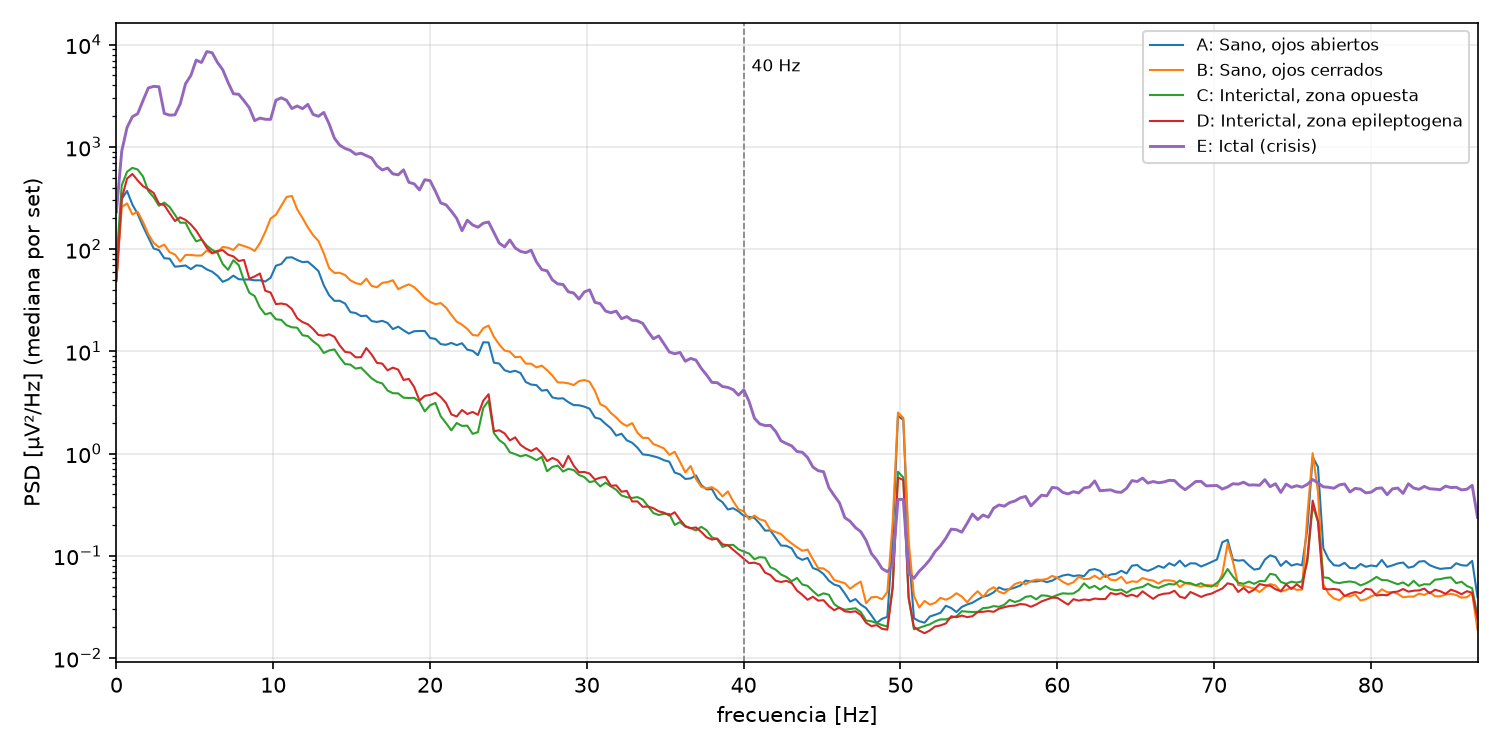
\includegraphics[width=0.85\textwidth]{etapa1/psd_welch_por_set.png}
  \caption{Densidad espectral de potencia (Welch, Hann de 512 muestras, 50~\% de solapamiento), mediana por
           set de Bonn, antes del filtro de 40 Hz.}
  \label{fig:psd_bonn}
\end{figure}

\begin{table}[ht]
\centering
\caption{Potencia relativa media por banda en cada set de Bonn (señal filtrada a 40 Hz). Cada fila suma 1.}
\label{tab:bonn_bandas}
\begin{tabular}{llrrrrr}
\toprule
Set & Descripción & delta & theta & alfa & beta & gamma \\
\midrule
A & sano, ojos abiertos     & 0,367 & 0,182 & 0,241 & 0,203 & 0,007 \\
B & sano, ojos cerrados     & 0,181 & 0,126 & \textbf{0,476} & 0,213 & 0,004 \\
C & interictal, zona opuesta & \textbf{0,668} & 0,214 & 0,071 & 0,044 & 0,002 \\
D & interictal, foco        & 0,602 & 0,253 & 0,100 & 0,044 & 0,001 \\
E & ictal                   & 0,248 & \textbf{0,405} & 0,174 & 0,171 & 0,003 \\
\bottomrule
\end{tabular}
\end{table}

La Tabla~\ref{tab:bonn_bandas} muestra que la \emph{distribución} de la potencia entre bandas también
cambia: en el set E la banda dominante es theta (40,5~\%), mientras que en los interictales intracraneales
(C, D) domina delta (60--67~\%). El espectrograma de un segmento ictal (Figura~\ref{fig:espectrograma_bonn})
muestra además que la frecuencia de la descarga no es constante a lo largo del tiempo.

\begin{figure}[ht]
  \centering
  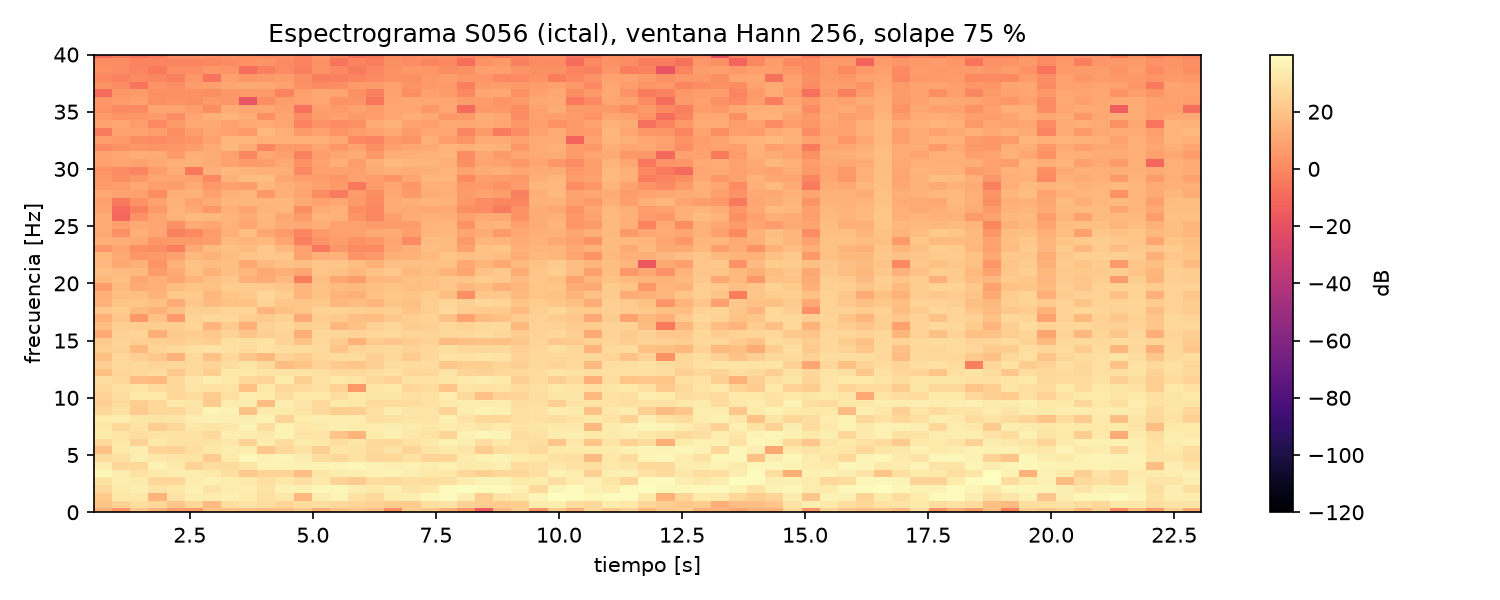
\includegraphics[width=0.85\textwidth]{etapa1/espectrograma_S056.png}
  \caption{Espectrograma del segmento ictal S056 de Bonn (Hann de 256 muestras, 75~\% de solapamiento).}
  \label{fig:espectrograma_bonn}
\end{figure}

\chapter{Datos}
\label{cap:datos}

Se usan dos bases públicas con propósitos complementarios. La de Bonn es chica, limpia y balanceada:
sirve para estudiar el espectro de las crisis y para ilustrar la teoría (softmax, simplex, KKT) con un
problema de tres clases. CHB-MIT tiene registros continuos de muchas horas, con el desbalance real entre
crisis y actividad normal: es donde se evalúa la detección como se haría en la clínica. Las dos se bajaron
solo de sus fuentes oficiales.

\section{Base de Bonn}
\label{sec:bonn}

\subsection{Descripción}

La base de la Universidad de Bonn \parencite{andrzejak2001} tiene cinco conjuntos (A a E) de 100 segmentos
de un canal cada uno. Cada segmento tiene $N = 4097$ muestras a $f_s = 173{,}61$~Hz, es decir 23,6~s, con
12 bits de resolución. Los segmentos se cortaron de registros continuos de varios canales, después de
revisarlos visualmente para descartar artefactos de movimiento y de los ojos.

\begin{table}[ht]
\centering
\caption{Conjuntos de la base de Bonn y clases usadas en este trabajo.}
\label{tab:bonn_sets}
\begin{tabular}{cclll}
\toprule
Set & Archivo & Registro & Estado & Clase \\
\midrule
A & Z & superficie, 5 voluntarios sanos & vigilia, ojos abiertos & \multirow{2}{*}{sano} \\
B & O & superficie, 5 voluntarios sanos & vigilia, ojos cerrados & \\
C & N & intracraneal, hemisferio opuesto al foco & entre crisis & \multirow{2}{*}{interictal} \\
D & F & intracraneal, zona epileptógena & entre crisis & \\
E & S & intracraneal, zonas con actividad ictal & durante la crisis & ictal \\
\bottomrule
\end{tabular}
\end{table}

Se agrupan en tres clases: \textbf{sano} (A+B, 200 segmentos), \textbf{interictal} (C+D, 200) e
\textbf{ictal} (E, 100). Es un problema balanceado, donde la exactitud sí tiene sentido.

La Figura~\ref{fig:bonn_ejemplos} muestra un segmento de cada set. Ya a simple vista se distinguen el ritmo alfa
regular del set B (ojos cerrados), las ondas lentas y las puntas aisladas de los interictales (C y D) y, en el
set E, la descarga de puntas casi periódicas, de unos 2 por segundo y hasta 800~µV, que describe la
ecuación~\eqref{eq:descarga}. Las escalas verticales son distintas en cada panel: la amplitud del set E es de
cinco a diez veces la de los sanos.

\begin{figure}[ht]
  \centering
  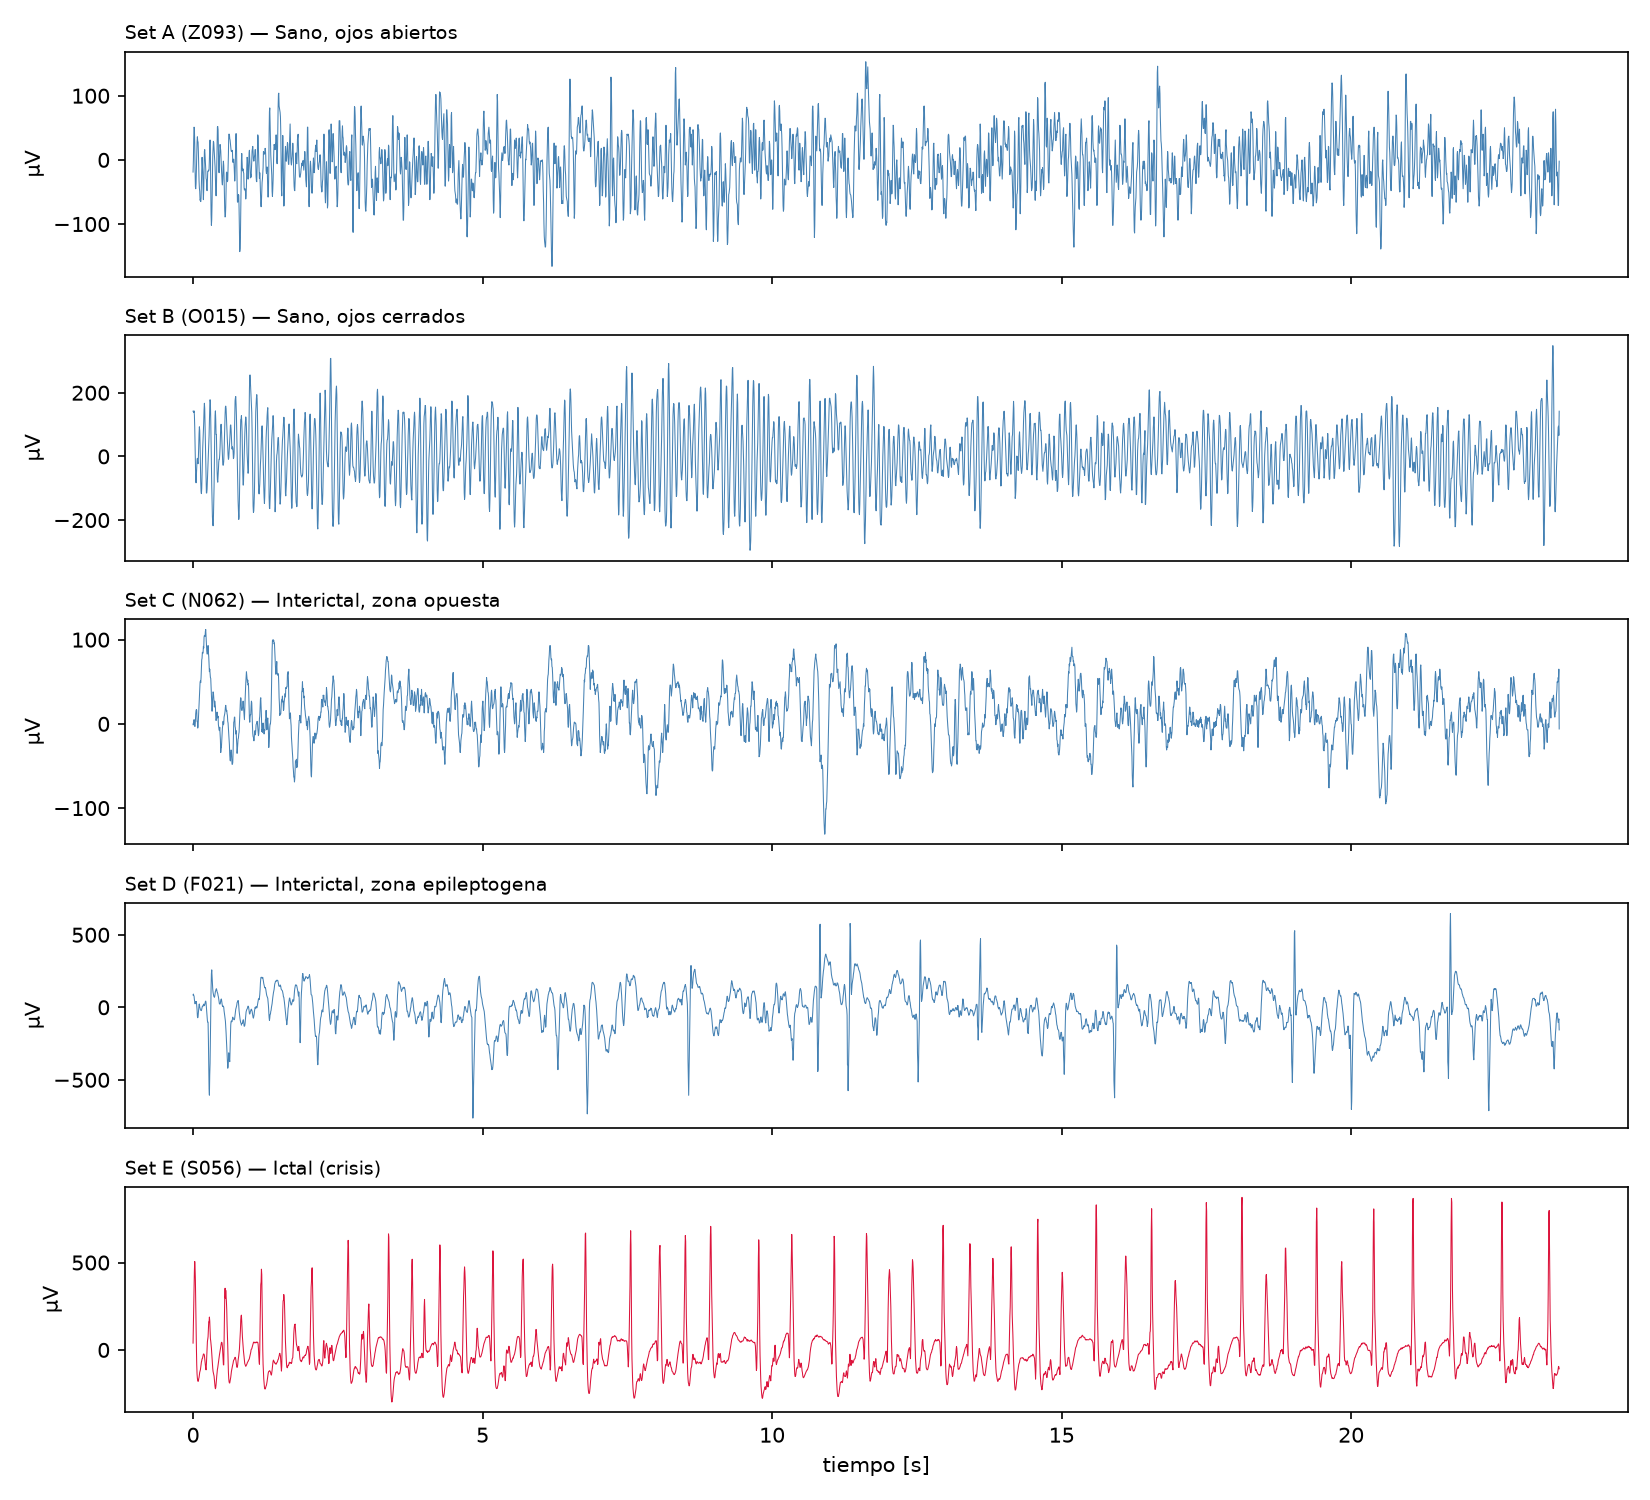
\includegraphics[width=\textwidth]{etapa1/ejemplos_por_set.png}
  \caption{Un segmento de 23,6~s de cada set de Bonn, en microvoltios. En rojo, el segmento ictal S056, el mismo del
           espectrograma de la Figura~\ref{fig:espectrograma_bonn}.}
  \label{fig:bonn_ejemplos}
\end{figure}

\subsection{Controles de calidad}

\begin{itemize}
  \item \textbf{Amplitud.} El desvío estándar del set E es 341~µV; el de los demás está entre 48 (A) y
        90~µV (D). La diferencia de amplitud, por sí sola, ya separa bastante las crisis (Capítulo~\ref{cap:fenomeno}).
  \item \textbf{Saturación.} El conversor de 12 bits satura en $\pm 2047$. Tres segmentos alcanzan ese valor:
        F009 (52 muestras) y S059 y S065 (20 muestras entre ambos). Son pocas muestras y se conservan.
  \item \textbf{Contenido por encima de 40 Hz.} Las series descargables no tienen aplicado el pasabajos de
        40~Hz del artículo original. La energía por encima de 40~Hz es como máximo el 0,39~\% del total (set A),
        así que aplicar el filtro casi no cambia las señales.
\end{itemize}

\subsection{Limitación}

La base no dice a qué paciente pertenece cada segmento. Al hacer validación cruzada, segmentos del mismo
paciente pueden quedar a la vez en entrenamiento y en prueba, de modo que las métricas sobrestiman lo que
pasaría con un paciente nuevo. Además, los segmentos se eligieron sin artefactos y cada clase viene de
condiciones de registro distintas (superficie contra intracraneal), lo que facilita la separación. Bonn sirve
para estudiar el fenómeno, no para medir el desempeño clínico; eso se hace con CHB-MIT.

\section{Base CHB-MIT}
\label{sec:chbmit}

\subsection{Descripción}

La base CHB-MIT \parencite{shoeb2009,guttag2010}, distribuida por PhysioNet \parencite{goldberger2000} con
licencia ODC-By~1.0, tiene registros de EEG de superficie de pacientes pediátricos del Children's Hospital
Boston, tomados durante varios días después de suspender la medicación para registrar crisis antes de una
posible cirugía. Las señales están muestreadas a 256~Hz con 16 bits, en el sistema internacional 10-20 con
montaje bipolar. El inicio y el fin de cada crisis fueron anotados por especialistas, con resolución de
1~s, en los archivos \texttt{chbNN-summary.txt}.

Se usan seis pacientes: chb01, chb02, chb03, chb05, chb08 y chb10, con 200 archivos EDF (8,8~GB). Todos
los archivos se verificaron contra las sumas SHA-256 publicadas por PhysioNet. La Tabla~\ref{tab:pacientes}
resume los datos.

\begin{table}[ht]
\centering
\caption{Pacientes de CHB-MIT usados. Ventanas de 4~s; ``borde'' son las que tocan una crisis solo en parte.}
\label{tab:pacientes}
\begin{tabular}{lcrrrrrrr}
\toprule
Paciente & Sexo, edad & Archivos & Horas & Ventanas & Ictales & Borde & Crisis & Duración [s] \\
\midrule
chb01 & F, 11  & 42 & 40,6 & 36\,496 & 107 & 8  & 7 & 27--101 \\
chb02 & M, 11  & 36 & 35,3 & 31\,739 & 41  & 4  & 3 & 9--82 \\
chb03 & F, 14  & 38 & 38,0 & 34\,201 & 96  & 10 & 7 & 47--69 \\
chb05 & F, 7   & 39 & 39,0 & 35\,102 & 136 & 7  & 5 & 96--120 \\
chb08 & M, 3,5 & 20 & 20,0 & 18\,005 & 226 & 8  & 5 & 134--264 \\
chb10 & M, 3   & 25 & 50,0 & 45\,020 & 105 & 12 & 7 & 35--89 \\
\midrule
Total &        & 200 & 222,8 & 200\,563 & 711 & 49 & 34 & \\
\bottomrule
\end{tabular}
\end{table}

Las 34 crisis suman 2940~s: el \textbf{0,366~\%} del tiempo registrado. Hay unas 280 ventanas sin crisis por
cada ventana ictal. Las crisis de chb08 son las más largas (hasta 264~s) y las de chb02, las más cortas (9~s).

\subsection{Canales}

Se usan los 18 canales del montaje bipolar ``doble banana'', comunes a todos los archivos de estos pacientes:
\begin{center}
\small
FP1-F7, F7-T7, T7-P7, P7-O1, FP1-F3, F3-C3, C3-P3, P3-O1, FP2-F4, F4-C4, C4-P4, P4-O2,\\
FP2-F8, F8-T8, T8-P8, P8-O2, FZ-CZ, CZ-PZ.
\end{center}
Los archivos tienen un canal 23 que repite T8-P8 y se descarta.

\section{Preprocesamiento de CHB-MIT}
\label{sec:preproc}

El script \texttt{scripts/preprocesar\_chbmit.py} procesa cada EDF una sola vez, en paralelo, y guarda un
archivo \texttt{.npz} por registro. Los pasos son:
\begin{enumerate}
  \item \textbf{Lectura} de los 18 canales con MNE y conversión a µV.
  \item \textbf{Filtrado} pasabanda Butterworth de orden 4 entre 0,5 y 40~Hz, de fase cero
        (\texttt{sosfiltfilt}), sobre el registro completo para evitar efectos de borde en cada ventana.
  \item \textbf{Ventanas} consecutivas, sin solapamiento, de $L = 4$~s (1024 muestras).
  \item \textbf{Espectrograma} de cada ventana y canal: Hann de 256 muestras (1~s), salto de 128 (0,5~s), lo que
        da 7 cuadros. Se guardan las frecuencias de 1 a 40~Hz (40 valores) en escala $\log_{10}$: un tensor de
        $18\times40\times7$ por ventana, que es la entrada de la CNN.
  \item \textbf{Potencia por banda}: el promedio de los 7 cuadros es la PSD de Welch; se integra con la regla del
        trapecio en las 5 bandas clínicas (delta 0,5--4, theta 4--8, alfa 8--13, beta 13--30 y gamma 30--40~Hz) y
        se toma $\log_{10}$. Resultan 90 atributos por ventana, la entrada de los modelos convexos.
  \item \textbf{Etiquetas}: para la ventana $w = [t_0, t_0 + L)$ y las crisis anotadas $[a_j, b_j]$,
        \begin{equation}
          y(w) =
          \begin{cases}
            1 \ \text{(ictal)} & \text{si } a_j \le t_0 \text{ y } t_0 + L \le b_j \text{ para algún } j, \\
            \text{borde} & \text{si la ventana se superpone con una crisis pero no está contenida}, \\
            0 \ \text{(sin crisis)} & \text{en otro caso.}
          \end{cases}
        \end{equation}
  \item \textbf{Amplitud máxima} de cada ventana, para analizar artefactos.
\end{enumerate}
Resultan 200\,563 ventanas: 711 ictales, 49 de borde y 199\,803 sin crisis.

Las ventanas de borde mezclan los dos estados, y la anotación tiene unos segundos de incertidumbre, así que no se
usan para entrenar. No se descartan ventanas por artefactos: un detector real tiene que funcionar con ellos.

\section{Análisis exploratorio}
\label{sec:exploratorio}

\subsection{Una crisis en la señal}

La Figura~\ref{fig:chb01_cruda} muestra los 18 canales alrededor de la primera crisis de chb01 (archivo
chb01\_03, de 2996 a 3036~s). Antes de la crisis se ven ráfagas de 10--14~Hz en los canales frontales, que son
actividad normal. Al empezar la crisis aparece una descarga rítmica de gran amplitud en casi todos los canales.
Después del fin anotado queda actividad lenta de gran amplitud: es el estado \emph{post-ictal}, que se etiqueta
como ``sin crisis'' y es una fuente esperable de falsas alarmas.

\begin{figure}[ht]
  \centering
  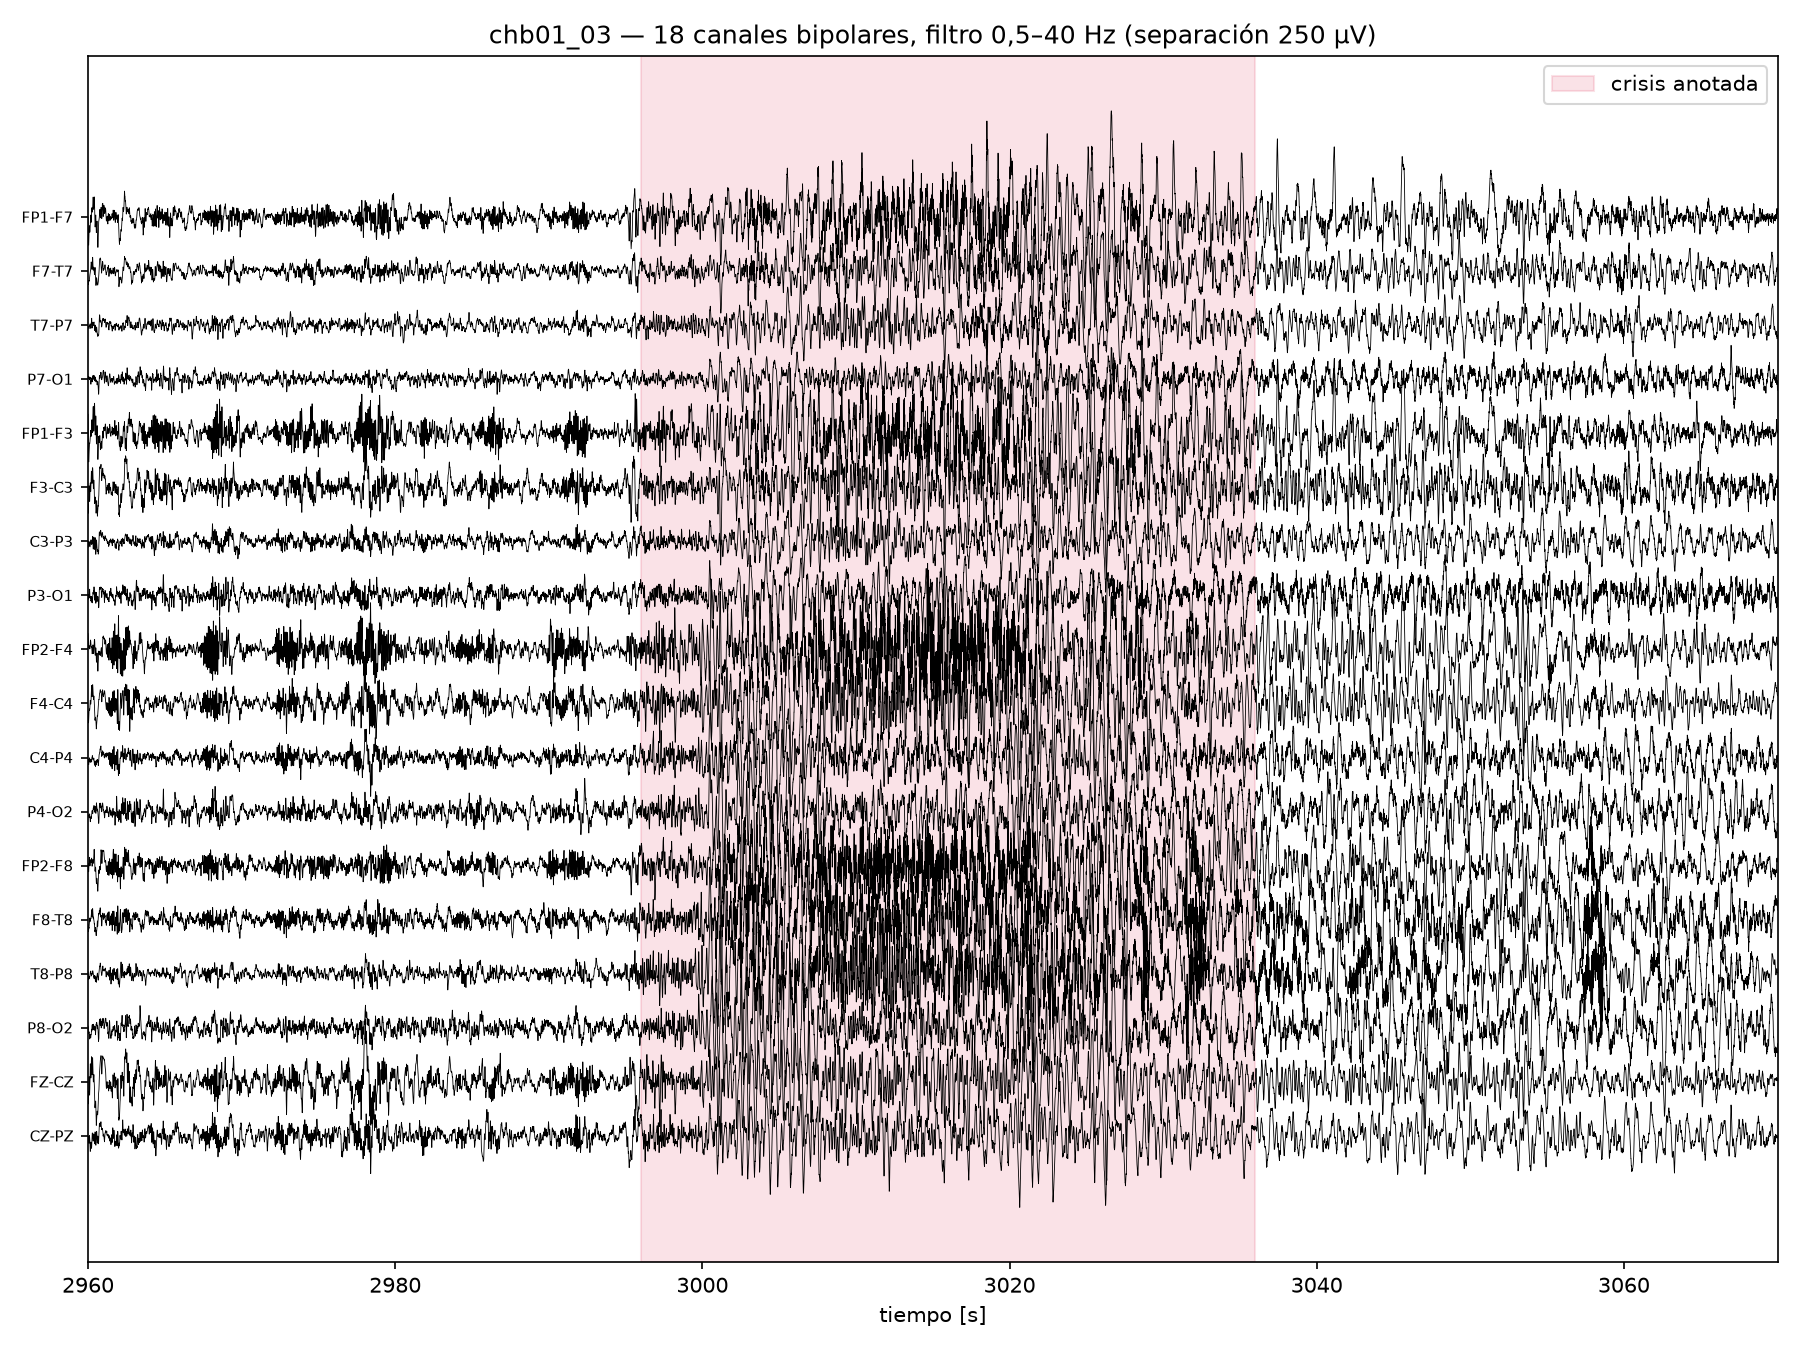
\includegraphics[width=\textwidth]{etapa2/chb01_03_crisis_cruda.png}
  \caption{Registro chb01\_03, 18 canales bipolares filtrados entre 0,5 y 40~Hz. La banda sombreada es la crisis
           anotada (2996--3036~s).}
  \label{fig:chb01_cruda}
\end{figure}

El espectrograma del canal con mayor amplitud durante la crisis (Figura~\ref{fig:chb01_espectrograma}) muestra
que la potencia sube en todo el rango de 1 a 40~Hz, sobre todo por debajo de 8~Hz, que es la descarga rítmica de
la ecuación~\eqref{eq:descarga}. Las líneas horizontales cerca de 16 y 32~Hz están presentes en todo el registro:
son interferencia de banda angosta del equipo, el término $\eta_c(t)$ del modelo~\eqref{eq:modelo_eeg}. Durante la
crisis quedan tapadas por la descarga.

\begin{figure}[ht]
  \centering
  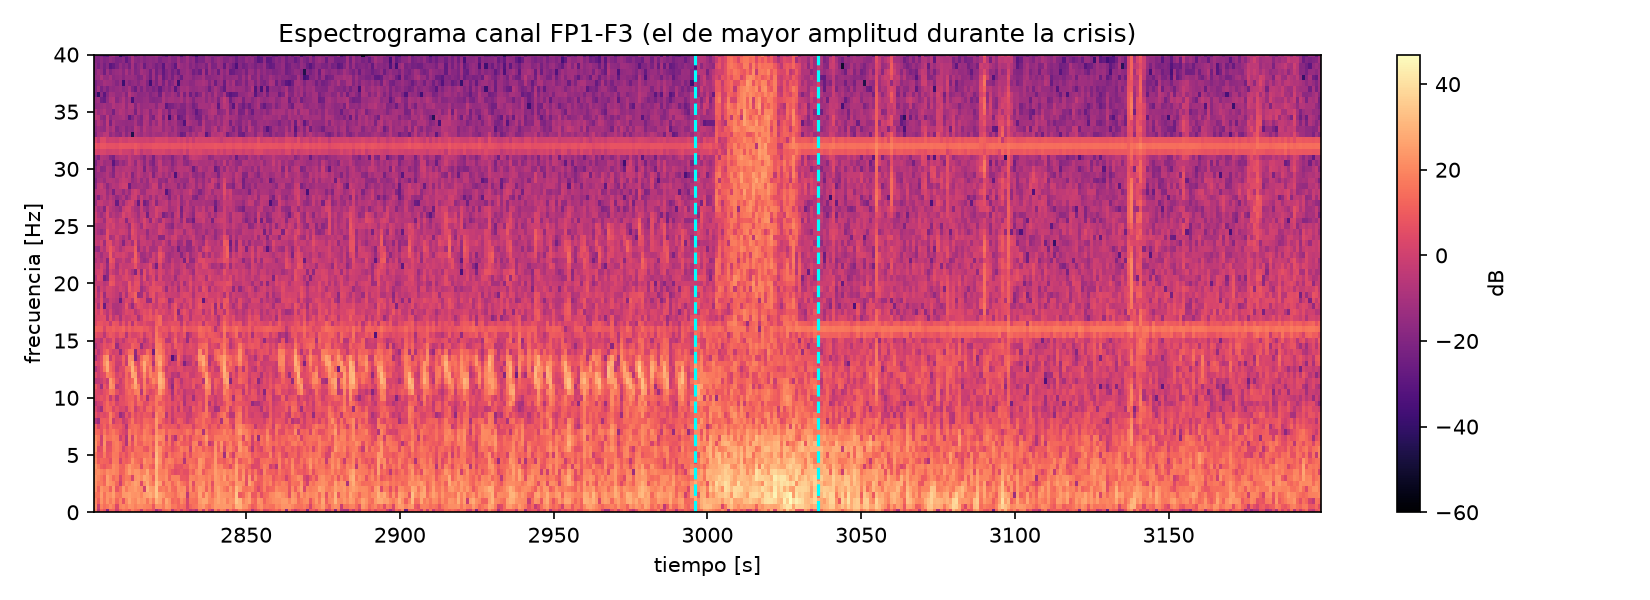
\includegraphics[width=\textwidth]{etapa2/chb01_03_espectrograma.png}
  \caption{Espectrograma (Hann de 2~s, 50~\% de solapamiento) alrededor de la crisis de chb01\_03. Las líneas
           punteadas marcan el inicio y el fin anotados.}
  \label{fig:chb01_espectrograma}
\end{figure}

\subsection{Potencia por banda y variabilidad entre pacientes}

La Figura~\ref{fig:bandas_pacientes} compara la potencia por banda (promedio de los 18 canales) en ventanas con y
sin crisis, para cada paciente, y la Tabla~\ref{tab:dif_log} resume la diferencia de las medias en escala
logarítmica.

\begin{figure}[ht]
  \centering
  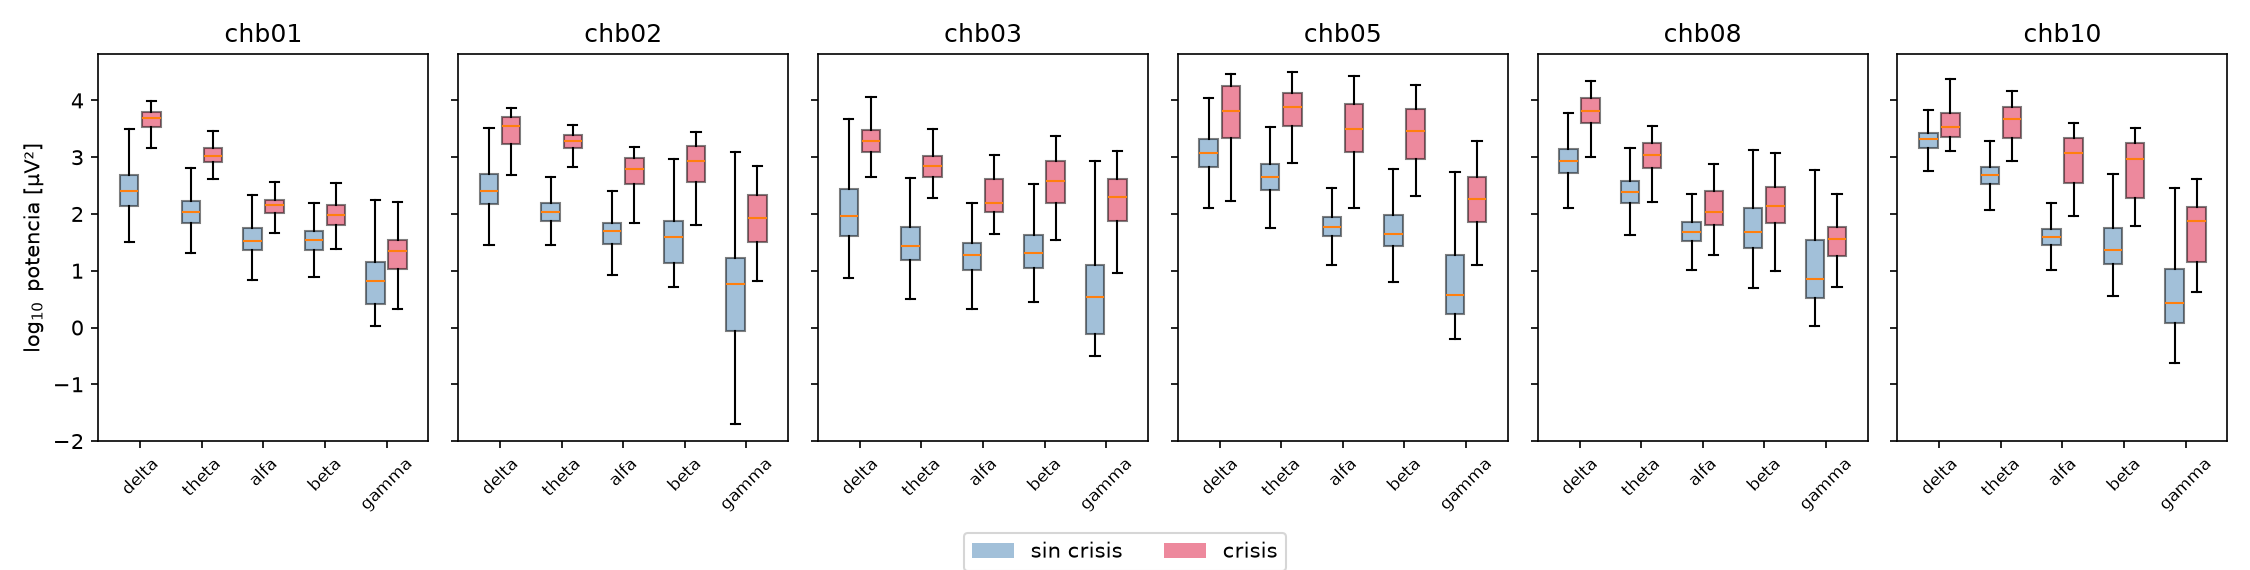
\includegraphics[width=\textwidth]{etapa2/potencia_bandas_por_paciente.png}
  \caption{$\log_{10}$ de la potencia por banda, promedio de los 18 canales, en ventanas sin crisis (azul) y con
           crisis (rojo), por paciente.}
  \label{fig:bandas_pacientes}
\end{figure}

\begin{table}[ht]
\centering
\caption{Diferencia media de $\log_{10}$ de la potencia entre ventanas con y sin crisis. Un valor de 1 equivale a
10 veces más potencia. En negrita, la banda de mayor aumento en cada paciente.}
\label{tab:dif_log}
\begin{tabular}{lrrrrr}
\toprule
Paciente & delta & theta & alfa & beta & gamma \\
\midrule
chb01 & \textbf{1,19} & 0,98 & 0,55 & 0,41 & 0,43 \\
chb02 & 0,99 & 1,19 & 1,05 & \textbf{1,25} & 1,24 \\
chb03 & 1,25 & 1,33 & 1,02 & 1,18 & \textbf{1,63} \\
chb05 & 0,68 & 1,20 & \textbf{1,69} & 1,67 & 1,47 \\
chb08 & \textbf{0,83} & 0,62 & 0,40 & 0,39 & 0,47 \\
chb10 & 0,34 & 0,91 & \textbf{1,33} & 1,29 & 1,07 \\
\bottomrule
\end{tabular}
\end{table}

Tres observaciones guían el resto del trabajo:
\begin{enumerate}
  \item \textbf{La potencia sube siempre.} En todos los pacientes y en todas las bandas, entre $10^{0{,}34} \approx 2$ y
        $10^{1{,}69} \approx 50$ veces. Es lo que predice el modelo aditivo (ecuación~\eqref{eq:dif_log}) y justifica usar la
        potencia por banda como atributo.
  \item \textbf{La banda que más sube depende del paciente.} Delta y theta en chb01 y chb08; alfa y beta en chb05 y
        chb10. Corresponde a frecuencias fundamentales $f_0$ distintas de la descarga. Un detector que sirva para
        pacientes nuevos tiene que combinar bandas.
  \item \textbf{El nivel basal también depende del paciente.} La potencia delta de chb10 \emph{sin} crisis (mediana
        $\approx 3{,}3$ en $\log_{10}$) está cerca de la de chb01 \emph{con} crisis ($\approx 3{,}7$). Un umbral fijo sobre una
        banda no sirve para todos. Es el término $2\log g_{p,c}$ del modelo, y motiva la calibración por paciente.
\end{enumerate}
chb08 es el paciente con menor aumento (0,4 a 0,8): sus crisis, largas y de menor amplitud relativa, son las más
difíciles de detectar.

\subsection{Artefactos de amplitud}

La mediana de la amplitud máxima por ventana sin crisis va de 178~µV (chb03) a 344~µV (chb08), y su percentil 99,
de 878 a 1430~µV. El percentil 99 de las ventanas sin crisis es del mismo orden que la mediana de las ventanas con
crisis (469 a 1252~µV): hay muchas ventanas normales con artefactos de amplitud comparable a una crisis, y la
amplitud sola no alcanza para detectar.

\section{Particiones}
\label{sec:particiones}

Las ventanas consecutivas de un registro están muy correlacionadas. Si se reparten al azar entre entrenamiento
y prueba, el modelo puede reconocer el registro y las métricas salen infladas (fuga de información). En CHB-MIT
todas las particiones son \emph{por paciente}.
\begin{itemize}
  \item \textbf{Bonn:} validación cruzada estratificada de 10 particiones, repetida 5 veces (con la limitación de la
        Sección~\ref{sec:bonn}).
  \item \textbf{CHB-MIT, LOPO:} 6 particiones, cada una deja afuera un paciente. Para los modelos convexos.
  \item \textbf{CHB-MIT, partición fija:} para la CNN y la comparativa de optimizadores, donde repetir 6 particiones
        con 6 optimizadores, 3 tasas y 5 semillas sería demasiado costoso sin GPU. Se eligió para que los tres
        conjuntos tengan una cantidad parecida de segundos de crisis (Tabla~\ref{tab:particion}).
\end{itemize}

\begin{table}[ht]
\centering
\caption{Partición fija por paciente de CHB-MIT.}
\label{tab:particion}
\begin{tabular}{llrrrr}
\toprule
Conjunto & Pacientes & Horas & Ventanas & Ictales & Crisis \\
\midrule
Entrenamiento & chb02, chb05, chb08 & 94,3 & 84\,846 & 403 & 13 \\
Validación    & chb01               & 40,6 & 36\,496 & 107 & 7 \\
Prueba        & chb03, chb10        & 88,0 & 79\,221 & 201 & 14 \\
\bottomrule
\end{tabular}
\end{table}

El conjunto de validación se usa para elegir la tasa de aprendizaje, la época de parada y el umbral de
Neyman-Pearson. El de prueba se evalúa una sola vez con el modelo elegido.

\section{Calibración por paciente}
\label{sec:calibracion}

Según el modelo~\eqref{eq:modelo_eeg}, el logaritmo de la potencia de cada canal y banda tiene un término
$2\log g_{p,c}$ que depende solo del paciente. Para eliminarlo, a cada atributo de cada paciente se le resta su
mediana sobre \emph{todas} las ventanas de ese paciente:
\begin{equation}
  \tilde x_{t,j} = x_{t,j} - \operatorname{mediana}_{u \in \text{paciente}(t)}\, x_{u,j}.
  \label{eq:calibracion}
\end{equation}
Se usa la mediana y no la media porque es robusta: las crisis son menos del 1~\% de las ventanas y casi no la
mueven, de modo que estima el nivel basal. La calibración \emph{no usa etiquetas}. En la práctica equivale a
registrar un rato al paciente nuevo antes de usar el detector, lo cual es razonable en una unidad de monitoreo,
donde los registros duran días.

La misma calibración se aplica al espectrograma de entrada de la CNN: a cada canal y frecuencia se le resta la
mediana del paciente.

Hay que notar que, en los pacientes de prueba, la mediana se calcula con todo su registro, incluido el futuro. Un
sistema en línea tendría que usar una mediana de las primeras horas o una ventana móvil; como la mediana es estable
(depende del nivel basal, no de las crisis), no se espera que el resultado cambie mucho, pero no se verificó.

\chapter{Métricas de evaluación}
\label{cap:metricas}

Un detector de crisis produce, para cada ventana, un puntaje $s(\vx)$ y una decisión
$\hat y = \mathds{1}[s(\vx) > \tau]$. Este capítulo define cómo se mide su desempeño: primero por ventana
(matriz de confusión, sensibilidad, especificidad, curva ROC), después por evento, que es lo que importa en la
clínica (crisis detectadas, falsas alarmas por hora, latencia), y finalmente cómo se comparan modelos entre sí con
tests estadísticos. Las definiciones son las que implementa \texttt{scripts/metricas.py}.

\section{Matriz de confusión}

Para un problema binario, con la clase positiva ``crisis'', cada ventana cae en una de cuatro celdas:
\begin{center}
\begin{tabular}{lcc}
\toprule
 & predicho: sin crisis & predicho: crisis \\
\midrule
real: sin crisis & $TN$ (verdadero negativo) & $FP$ (falso positivo) \\
real: crisis     & $FN$ (falso negativo)    & $TP$ (verdadero positivo) \\
\bottomrule
\end{tabular}
\end{center}
Con $n_1 = TP + FN$ positivos y $n_0 = TN + FP$ negativos. Todas las métricas por ventana son cocientes entre estas
cuatro cantidades. En el problema de $K$ clases (Bonn) la matriz es de $K \times K$: la entrada $(i,j)$ cuenta los
ejemplos de clase real $i$ predichos como $j$, y la diagonal son los aciertos.

\section{Sensibilidad, especificidad y valor predictivo}

\begin{align}
  \text{sensibilidad} &= \frac{TP}{TP + FN} = P(\hat y = 1 \mid y = 1) && \text{(tasa de verdaderos positivos, TPR)} \\
  \text{especificidad} &= \frac{TN}{TN + FP} = P(\hat y = 0 \mid y = 0) && \text{(igual a $1 - $ FPR, tasa de falsos positivos)} \\
  \text{VPP} &= \frac{TP}{TP + FP} = P(y = 1 \mid \hat y = 1) && \text{(valor predictivo positivo, precisión)} \\
  F_1 &= \frac{2\,\text{VPP}\cdot\text{sensibilidad}}{\text{VPP} + \text{sensibilidad}}
\end{align}

La sensibilidad y la especificidad están condicionadas a la clase \emph{real}, de modo que no dependen de la proporción
de positivos: son propiedades del detector. El VPP está condicionado a la \emph{decisión} y sí depende de esa
proporción. Por la regla de Bayes, con prevalencia $\pi_1$,
\begin{equation}
  \text{VPP} = \frac{\text{sens}\cdot\pi_1}{\text{sens}\cdot\pi_1 + (1 - \text{espec})\,(1 - \pi_1)}.
  \label{eq:vpp_bayes}
\end{equation}
Con $\pi_1 = 0{,}0025$ (proporción de ventanas ictales en los pacientes de prueba), sensibilidad 0,63 y
especificidad 0,9964 (los valores de la CNN final), el VPP es apenas 0,31: \emph{de cada tres alarmas por ventana,
dos son falsas}, aunque la especificidad parezca altísima.

En el caso de $K$ clases se calcula la sensibilidad y la especificidad de cada clase contra el resto (\emph{uno contra
todos}): para la clase $k$, $TP_k$ son los ejemplos de clase $k$ predichos como $k$, y así sucesivamente.

\subsection{Por qué la exactitud no sirve}
\label{sec:accuracy}

La exactitud, $(TP + TN)/(n_0 + n_1)$, es un promedio de la sensibilidad y la especificidad ponderado por la
prevalencia:
\begin{equation}
  \text{exactitud} = \pi_1\cdot\text{sensibilidad} + (1 - \pi_1)\cdot\text{especificidad}.
\end{equation}
Con $\pi_1 \approx 0{,}0025$, la sensibilidad casi no pesa. Un ejemplo concreto con los pacientes de prueba (201 ventanas
ictales y 78\,998 sin crisis):
\begin{itemize}
  \item un ``detector'' que \emph{nunca} declara crisis tiene exactitud $78\,998/79\,199 = 99{,}75~\%$;
  \item la CNN final, que detecta 11 de las 14 crisis, tiene exactitud $99{,}55~\%$.
\end{itemize}
El detector inútil le gana en exactitud al útil. Por eso en este trabajo la exactitud solo se informa en Bonn, donde
las clases están balanceadas (200, 200 y 100 segmentos), junto con la exactitud balanceada (promedio de las
sensibilidades de cada clase) y el $F_1$ macro.

\section{Curva ROC}
\label{sec:roc}

Las métricas anteriores dependen del umbral $\tau$. La curva ROC (\emph{receiver operating characteristic}) muestra
todos los umbrales a la vez \parencite{fawcett2006}:
\begin{equation}
  \text{ROC} = \Big\{\big(\text{FPR}(\tau),\ \text{TPR}(\tau)\big) : \tau \in \R\Big\},
  \qquad
  \text{FPR}(\tau) = P(s > \tau \mid y = 0),\quad \text{TPR}(\tau) = P(s > \tau \mid y = 1).
\end{equation}
Cuando $\tau$ baja desde $+\infty$ hasta $-\infty$, la curva va de $(0,0)$ (nunca detectar) a $(1,1)$ (detectar
siempre). Propiedades que se usan en el trabajo:
\begin{itemize}
  \item \textbf{Invariancia ante transformaciones crecientes.} Si $g$ es estrictamente creciente, $g(s)$ tiene la misma
        curva ROC que $s$. En particular da igual usar la probabilidad de la sigmoide o el puntaje antes de ella, y
        la curva no cambia por el peso de las clases en el entrenamiento, que solo desplaza los puntajes.
  \item \textbf{Independencia de la prevalencia.} Ambos ejes están condicionados a la clase real.
  \item \textbf{La diagonal} $\text{TPR} = \text{FPR}$ corresponde a decidir al azar. Una curva por debajo indica un puntaje
        con el signo invertido.
  \item \textbf{La pendiente} en cada punto es la razón de verosimilitud del puntaje,
        $q_1(\tau)/q_0(\tau)$ (ecuación~\eqref{eq:pendiente_roc}). Si el puntaje es una función creciente de la razón de
        verosimilitud, la curva es cóncava.
\end{itemize}

\subsection{Área bajo la curva}

El área bajo la curva (AUC) resume la curva en un número. Su interpretación probabilística es la más útil.

\begin{proposicion}
\label{prop:auc}
Sean $\vx^+$ un positivo y $\vx^-$ un negativo elegidos al azar e independientes. Si el puntaje es continuo,
\begin{equation}
  \text{AUC} = \int_0^1 \text{TPR}\,d(\text{FPR}) = P\big(s(\vx^+) > s(\vx^-)\big).
\end{equation}
\end{proposicion}
\begin{proof}
Sea $q_0$ la densidad del puntaje en los negativos. Parametrizando la curva por el umbral,
$d(\text{FPR}) = -q_0(\tau)\,d\tau$, y al recorrer FPR de 0 a 1 el umbral va de $+\infty$ a $-\infty$:
\[
  \text{AUC} = \int_{-\infty}^{\infty} \text{TPR}(\tau)\,q_0(\tau)\,d\tau
  = \int_{-\infty}^{\infty} P(s^+ > \tau)\,q_0(\tau)\,d\tau
  = P(s^+ > s^-),
\]
porque la última integral es la probabilidad de que $s^+$ supere a un $s^-$ con densidad $q_0$.
\end{proof}

Con datos, la versión empírica es la proporción de pares (positivo, negativo) bien ordenados, contando los empates
como medio:
\begin{equation}
  \widehat{\text{AUC}} = \frac{1}{n_0 n_1}\sum_{i:\,y_i = 1}\ \sum_{j:\,y_j = 0}
  \Big(\mathds{1}[s_i > s_j] + \tfrac12\mathds{1}[s_i = s_j]\Big) = \frac{U}{n_0 n_1},
  \label{eq:auc_mw}
\end{equation}
donde $U$ es el estadístico de Mann-Whitney. Un AUC de 0,5 es azar y 1 es separación perfecta. Para $K$ clases se
informa el AUC de cada clase contra el resto.

\subsection{La zona útil de la curva}
\label{sec:zona_util}

El AUC promedia sobre \emph{todos} los valores de FPR con el mismo peso, pero en un monitor de crisis solo interesa
una parte mínima de la curva. Con ventanas de 4 s hay 900 ventanas por hora; un FPR de 1~\% son 9 ventanas falsas por
hora, y uno de 5~\%, 45. El punto de operación razonable está en $\text{FPR} \lesssim 10^{-3}$, el 0,1~\% izquierdo
del eje. Dos detectores con el mismo AUC pueden ser muy distintos en esa zona: en el Capítulo~\ref{cap:convexos},
el paciente chb03 tiene AUC 0,95 con la regresión logística pero casi no detecta nada con menos de 1~\% de falsos
positivos. Por eso las curvas ROC de CHB-MIT se grafican con el eje horizontal en escala logarítmica (o simétrica
logarítmica, lineal cerca de cero) y, además del AUC, se informa la sensibilidad para un FPR fijo de $10^{-3}$.

\section{Métricas por evento}
\label{sec:eventos}

Al médico no le importa cuántas ventanas de 4 s se clasificaron bien, sino si se detectó cada crisis, cuántas veces
sonó la alarma sin motivo y con cuánto retraso. Las métricas por evento responden esas preguntas.

\subsection{Post-procesamiento: suavizado causal}

Antes de umbralizar, el puntaje de cada ventana se reemplaza por el promedio de las últimas $k = 3$ ventanas del mismo
registro (12 s):
\begin{equation}
  \tilde s_t = \frac{1}{\min(k, t)}\sum_{u = \max(1, t-k+1)}^{t} s_u.
\end{equation}
El filtro es \emph{causal}: solo usa el pasado, así que podría aplicarse en tiempo real. Una crisis dura en general
más de 12 s y produce puntajes altos sostenidos, mientras que muchos artefactos afectan una sola ventana; el promedio
atenúa estos últimos. El costo es un retardo de hasta dos ventanas en la detección.

\subsection{Definiciones}

Sean $[a_j, b_j]$ las crisis anotadas y $\hat y_t$ las decisiones por ventana después del suavizado.
\begin{itemize}
  \item \textbf{Crisis detectada:} al menos una ventana positiva se superpone con $[a_j, b_j]$.
  \item \textbf{Sensibilidad por evento:} crisis detectadas sobre crisis totales.
  \item \textbf{Alarma:} una racha de ventanas positivas consecutivas cuenta como una sola alarma. Es \emph{falsa} si no
        se superpone con ninguna crisis.
  \item \textbf{Falsas alarmas por hora (FA/h):} alarmas falsas dividido por las horas de registro fuera de las crisis.
  \item \textbf{Latencia:} desde el inicio anotado $a_j$ hasta el \emph{final} de la primera ventana positiva (la decisión
        sobre una ventana recién se puede tomar cuando termina). Se informa la mediana sobre las crisis detectadas.
\end{itemize}
Las ventanas de \emph{borde} (que tocan una crisis solo en parte) no se usan para entrenar ni para las métricas por
ventana, porque su etiqueta es ambigua; sí se usan en las métricas por evento, que trabajan sobre el registro completo.

\paragraph{Relación con las métricas por ventana.} Si las ventanas falsas fueran independientes, con tasa FPR, el
número esperado de alarmas falsas por hora sería como máximo $900\cdot\text{FPR}$; agruparlas en rachas lo reduce. En la
CNN final, las 282 ventanas falsas positivas de los pacientes de prueba (87,8 horas sin crisis) se agrupan en 119
alarmas: 3,2 ventanas falsas por hora, pero 1,36 alarmas falsas por hora.

\subsection{El compromiso clínico}

Las tres métricas por evento se mueven juntas con el umbral: bajarlo aumenta la sensibilidad por evento y reduce la
latencia, pero aumenta las FA/h. La curva de sensibilidad por evento en función de FA/h, que se obtiene variando
$\alpha$ en el umbral de Neyman-Pearson, es la versión clínica de la curva ROC y se presenta en el
Capítulo~\ref{cap:resultados}. Como referencia, en la literatura de detección específica por paciente con CHB-MIT
\parencite{shoeb2009} se reportan del orden de 96~\% de crisis detectadas con unas 2 falsas alarmas por día; en
detección para pacientes nuevos, sin entrenar con datos del paciente, el problema es mucho más difícil.

\section{Umbral de Neyman-Pearson}
\label{sec:umbral_np}

El umbral no se elige maximizando la exactitud ni el $F_1$, sino fijando de antemano la tasa de falsos positivos por
ventana tolerable, $\alpha$, y maximizando la sensibilidad bajo esa restricción. En la Sección~\ref{sec:neyman_pearson}
se demostró, con multiplicadores de Lagrange, que la solución es comparar el puntaje con el cuantil $1 - \alpha$ de su
distribución en la clase negativa. En la práctica:
\begin{enumerate}
  \item se calcula el puntaje suavizado de todas las ventanas sin crisis de un conjunto de calibración que \emph{no} se
        usa para evaluar (los pacientes de entrenamiento en LOPO; el de validación en la partición fija);
  \item se toma $\tau = $ cuantil empírico $1 - \alpha$ de esos puntajes, ecuación~\eqref{eq:umbral_np};
  \item se aplica ese $\tau$, sin cambios, a los pacientes de prueba.
\end{enumerate}
Se usa $\alpha = 10^{-3}$ (del orden de una ventana falsa por hora). En el Capítulo~\ref{cap:resultados} se muestra
el barrido de $\alpha$ entre $3\times10^{-5}$ y $3\times10^{-2}$.

\section{Esquemas de validación}
\label{sec:validacion}

Una métrica solo tiene sentido si se mide sobre datos que el modelo no usó para entrenar ni para elegir
hiperparámetros. En EEG hay una trampa adicional: ventanas del mismo paciente, e incluso consecutivas, son muy
parecidas entre sí. Si se mezclan al azar en entrenamiento y prueba, el modelo puede aprender a reconocer al
paciente o al registro, y las métricas sobrestiman lo que pasaría con un paciente nuevo.
\begin{itemize}
  \item \textbf{Validación cruzada estratificada (Bonn).} Se divide en 10 partes con la misma proporción de clases,
        se entrena con 9 y se evalúa con la restante, rotando; se repite 5 veces con distinto orden. Como Bonn no
        informa a qué paciente pertenece cada segmento, no se puede separar por paciente: las métricas de Bonn son
        optimistas.
  \item \textbf{Dejar un paciente fuera (LOPO, CHB-MIT).} Se entrena con 5 pacientes y se evalúa con el sexto,
        rotando los 6. Mide la generalización a un paciente que el modelo nunca vio.
  \item \textbf{Partición fija (CHB-MIT).} Para la CNN, que tarda en entrenarse, se usa una sola partición por paciente:
        entrenamiento chb02, chb05 y chb08; validación chb01 (elección de tasa de aprendizaje, época y umbral); prueba
        chb03 y chb10, que se miran una sola vez al final. Los modelos convexos se evalúan también con esta partición
        para compararlos con la CNN.
\end{itemize}

\section{Comparación estadística entre modelos}
\label{sec:tests}

La CNN se entrena con varias semillas, y el resultado cambia de una a otra. Para decir que un optimizador es mejor que
otro no alcanza con comparar promedios: hay que ver si la diferencia es mayor que la variabilidad entre semillas.

\paragraph{Test de Mann-Whitney.} Dadas dos muestras independientes $a_1,\dots,a_{m}$ y $b_1,\dots,b_{m'}$ (por ejemplo,
el AUC de prueba de 5 semillas de cada optimizador), el estadístico $U$ cuenta los pares con $a_i > b_j$, igual que
en~\eqref{eq:auc_mw}. Bajo la hipótesis nula de que las dos muestras vienen de la misma distribución, todos los órdenes
son igualmente probables y la distribución de $U$ se calcula exactamente. Es un test no paramétrico: no supone
normalidad, algo razonable con 5 valores por grupo. Con $m = m' = 5$, el menor $p$ bilateral posible es
$2/\binom{10}{5} = 0{,}0079$, que se obtiene cuando las 5 semillas de un grupo superan a las 5 del otro ($U = 25$).

\paragraph{Comparaciones múltiples.} Al comparar un optimizador contra otros cinco se hacen cinco tests, y la
probabilidad de al menos un falso positivo crece. La corrección de Bonferroni exige $p < 0{,}05/5 = 0{,}01$ para cada
comparación.

\paragraph{Correlación de Spearman.} Para saber si el desempeño en validación predice el de prueba se usa la correlación
de Spearman $\rho$: la correlación de Pearson entre los rangos. Mide asociación monótona, no necesariamente lineal, y
es robusta a valores extremos.

\chapter{Fundamentos de optimización}
\label{cap:optimizacion}

Entrenar un modelo es resolver un problema de optimización: encontrar los parámetros $\vth$ que hacen
mínima una función de pérdida $J(\vth)$. Elegir un umbral de detección con una tasa de falsas alarmas
fija también lo es, pero con una restricción. Este capítulo reúne la teoría que se usa en el resto del
trabajo: óptimos locales y globales, convexidad, descenso por gradiente, multiplicadores de Lagrange,
condiciones de Karush-Kuhn-Tucker (KKT), dualidad, el simplex y la programación lineal. Al final se aplica
a tres problemas concretos del trabajo: la función softmax, el dual del SVM y el umbral de
Neyman-Pearson. La referencia principal es \textcite{boyd2004}; para los algoritmos, \textcite{nocedal2006}.

\section{Planteo general}

El problema de optimización en su forma general es
\begin{equation}
  \min_{\vth \in \R^d}\ f_0(\vth)
  \quad\text{sujeto a}\quad
  f_i(\vth) \le 0,\ i = 1,\dots,m, \qquad h_j(\vth) = 0,\ j = 1,\dots,p.
  \label{eq:problema_general}
\end{equation}
$f_0$ es la \emph{función objetivo}; las $f_i$ y $h_j$ definen el \emph{conjunto factible}
$\mathcal{D} = \{\vth : f_i(\vth) \le 0,\ h_j(\vth) = 0\}$. Maximizar $g$ es lo mismo que minimizar $-g$, así
que basta con estudiar la minimización. Si no hay restricciones, el problema es \emph{irrestricto}: es el
caso del entrenamiento de la regresión logística y de la red convolucional.

\section{Óptimo local y global}
\label{sec:local_global}

\begin{definicion}
Sea $J : \mathcal{D} \to \R$. Un punto $\vth^* \in \mathcal{D}$ es
\begin{itemize}
  \item \textbf{mínimo global} si $J(\vth^*) \le J(\vth)$ para todo $\vth \in \mathcal{D}$;
  \item \textbf{mínimo local} si existe $\varepsilon > 0$ tal que $J(\vth^*) \le J(\vth)$ para todo
        $\vth \in \mathcal{D}$ con $\lVert \vth - \vth^* \rVert < \varepsilon$;
  \item mínimo local o global \textbf{estricto} si la desigualdad es estricta para $\vth \neq \vth^*$.
\end{itemize}
\end{definicion}

Todo mínimo global es local; la recíproca es falsa en general. Un algoritmo que usa solo información
local (el valor de $J$ y de sus derivadas en el punto actual, como todos los que se usan en este trabajo)
no tiene forma de distinguir un mínimo local de uno global: si llega a un mínimo local, se queda ahí.

\subsection{Condiciones de optimalidad sin restricciones}

\begin{teorema}[Condición necesaria de primer orden]
\label{teo:primer_orden}
Si $J$ es diferenciable y $\vth^*$ es un mínimo local de $J$ en $\R^d$, entonces $\nabla J(\vth^*) = \mathbf{0}$.
\end{teorema}
\begin{proof}
Sea $\mathbf{d} = -\nabla J(\vth^*)$. Por la definición de derivada,
$J(\vth^* + t\mathbf{d}) = J(\vth^*) - t\lVert\nabla J(\vth^*)\rVert^2 + o(t)$. Si el gradiente no fuera nulo,
para $t > 0$ suficientemente chico se tendría $J(\vth^* + t\mathbf{d}) < J(\vth^*)$, lo que contradice que
$\vth^*$ es un mínimo local.
\end{proof}

Un punto con gradiente nulo se llama \emph{punto estacionario} o \emph{crítico}. Puede ser un mínimo, un
máximo o un \emph{punto silla}. Para distinguirlos hacen falta las derivadas segundas.

\begin{teorema}[Condiciones de segundo orden]
\label{teo:segundo_orden}
Sea $J$ dos veces diferenciable con continuidad y $\nabla J(\vth^*) = \mathbf{0}$.
\begin{enumerate}
  \item (Necesaria) Si $\vth^*$ es mínimo local, la Hessiana $\nabla^2 J(\vth^*)$ es semidefinida positiva.
  \item (Suficiente) Si $\nabla^2 J(\vth^*)$ es definida positiva, $\vth^*$ es un mínimo local estricto.
\end{enumerate}
\end{teorema}
\begin{proof}
Por el desarrollo de Taylor de segundo orden alrededor de un punto con gradiente nulo,
\[
  J(\vth^* + \mathbf{v}) = J(\vth^*) + \tfrac12\, \mathbf{v}^\top \nabla^2 J(\vth^*)\, \mathbf{v} + o(\lVert\mathbf{v}\rVert^2).
\]
(1) Si existiera $\mathbf{v}$ con $\mathbf{v}^\top \nabla^2 J\,\mathbf{v} < 0$, tomando $t\mathbf{v}$ con $t$ chico la
función bajaría, contradicción. (2) Si $\nabla^2 J \succ 0$, su menor autovalor $\mu$ es positivo y
$\mathbf{v}^\top\nabla^2 J\,\mathbf{v} \ge \mu\lVert\mathbf{v}\rVert^2$; para $\mathbf{v}$ chico el término
$o(\lVert\mathbf{v}\rVert^2)$ es menor que $\tfrac{\mu}{2}\lVert\mathbf{v}\rVert^2$, así que
$J(\vth^* + \mathbf{v}) > J(\vth^*)$.
\end{proof}

Estas condiciones son \emph{locales}: certifican que no hay nada mejor en un entorno de $\vth^*$, pero no
dicen nada sobre el resto del espacio. La convexidad es la propiedad que permite pasar de local a global.

\section{Conjuntos y funciones convexas}
\label{sec:convexidad}

\begin{definicion}
Un conjunto $\mathcal{D} \subseteq \R^d$ es \textbf{convexo} si para todo $\vth_1, \vth_2 \in \mathcal{D}$ y
$t \in [0,1]$, el punto $t\vth_1 + (1-t)\vth_2$ pertenece a $\mathcal{D}$. Una función $J : \mathcal{D} \to \R$,
con $\mathcal{D}$ convexo, es \textbf{convexa} si
\begin{equation}
  J\big(t\vth_1 + (1-t)\vth_2\big) \le t\,J(\vth_1) + (1-t)\,J(\vth_2)
  \qquad \forall\, \vth_1, \vth_2 \in \mathcal{D},\ t \in [0,1],
  \label{eq:def_convexa}
\end{equation}
y \textbf{estrictamente convexa} si la desigualdad es estricta cuando $\vth_1 \ne \vth_2$ y $t \in (0,1)$.
\end{definicion}

Geométricamente, la cuerda entre dos puntos del gráfico queda por encima del gráfico. Ejemplos que
aparecen en el trabajo: las normas $\lVert\vth\rVert$ y $\lVert\vth\rVert^2$, las funciones afines (convexas y
cóncavas a la vez), $\log(1 + e^z)$, la función \emph{log-sum-exp} $\log\sum_k e^{z_k}$ y la pérdida bisagra
$\max(0, 1 - z)$. Los poliedros $\{\vth : A\vth \le \mathbf{b}\}$ y el simplex
(Sección~\ref{sec:simplex}) son conjuntos convexos.

\begin{proposicion}[Caracterizaciones con derivadas]
\label{prop:caracterizacion}
Sea $J$ diferenciable en un dominio convexo abierto.
\begin{enumerate}
  \item $J$ es convexa si y solo si $J(\vth_2) \ge J(\vth_1) + \nabla J(\vth_1)^\top(\vth_2 - \vth_1)$ para todo
        $\vth_1, \vth_2$: el plano tangente queda siempre por debajo del gráfico.
  \item Si $J$ es dos veces diferenciable, $J$ es convexa si y solo si $\nabla^2 J(\vth) \succeq 0$ en todo
        punto. Si $\nabla^2 J(\vth) \succ 0$ en todo punto, $J$ es estrictamente convexa.
\end{enumerate}
\end{proposicion}

La condición (1) tiene una consecuencia inmediata: si $\nabla J(\vth^*) = \mathbf{0}$ y $J$ es convexa,
entonces $J(\vth) \ge J(\vth^*)$ para \emph{todo} $\vth$. Es decir, en una función convexa diferenciable
\emph{la condición de primer orden ya es suficiente para el óptimo global}. El teorema siguiente lo dice
sin pedir diferenciabilidad.

\begin{teorema}
\label{teo:local_global}
Sea $J$ convexa sobre un conjunto convexo $\mathcal{D}$.
\begin{enumerate}
  \item Todo mínimo local de $J$ es un mínimo global.
  \item El conjunto de minimizadores globales es convexo.
  \item Si $J$ es estrictamente convexa, tiene a lo sumo un minimizador.
\end{enumerate}
\end{teorema}
\begin{proof}
(1) Sea $\vth^*$ un mínimo local con radio $\varepsilon$ y supongamos que existe $\tilde\vth \in \mathcal{D}$ con
$J(\tilde\vth) < J(\vth^*)$. Para $t \in (0,1]$ el punto $\vth_t = (1-t)\vth^* + t\tilde\vth$ está en
$\mathcal{D}$ (convexidad del conjunto) y, por la convexidad de $J$,
\[
  J(\vth_t) \le (1-t)\,J(\vth^*) + t\,J(\tilde\vth) < J(\vth^*).
\]
Tomando $t < \varepsilon / \lVert\tilde\vth - \vth^*\rVert$ se tiene $\lVert\vth_t - \vth^*\rVert < \varepsilon$, y
$\vth_t$ es un punto del entorno con menor valor: contradicción.

(2) Si $\vth_1$ y $\vth_2$ son minimizadores con valor $J^*$, cualquier combinación convexa cumple
$J(t\vth_1 + (1-t)\vth_2) \le tJ^* + (1-t)J^* = J^*$, así que también es minimizador.

(3) Si $\vth_1 \neq \vth_2$ fueran dos minimizadores, la convexidad estricta daría
$J(\tfrac12\vth_1 + \tfrac12\vth_2) < J^*$, lo que es imposible.
\end{proof}

\begin{observacion}
El punto (2) da un criterio práctico para \emph{refutar} la convexidad: si se encuentran dos soluciones
$\vth_1, \vth_2$ con la misma pérdida y en su punto medio la pérdida es mayor, la función no es convexa.
Es el experimento que se hace con una red neuronal chica en el Capítulo~\ref{cap:convexos}: dos soluciones
con pérdida 0,041 tienen en su punto medio una pérdida de 0,596.
\end{observacion}

\subsection{Operaciones que preservan la convexidad}

Probar la convexidad desde la definición suele ser engorroso. En la práctica se usan reglas de composición:
\begin{itemize}
  \item La suma de funciones convexas, y el producto por un escalar no negativo, es convexa.
  \item Si $J$ es convexa, $\vth \mapsto J(A\vth + \mathbf{b})$ también lo es (composición con una función afín).
  \item El máximo puntual de funciones convexas es convexo.
\end{itemize}
Con estas reglas, la pérdida logística regularizada
$\frac1n\sum_i \big[\log(1 + e^{\vth^\top\tilde\vx_i}) - y_i\vth^\top\tilde\vx_i\big] + \frac{\lambda}{2}\lVert\vw\rVert^2$
es convexa (suma de convexas compuestas con funciones afines, más un término afín, más una norma al cuadrado),
y lo mismo pasa con el objetivo del SVM, $\frac12\lVert\vw\rVert^2 + C\sum_i\max(0, 1 - y_i(\vw^\top\vx_i + b))$.
En el Capítulo~\ref{cap:convexos} se calcula la Hessiana de la logística y se prueba que es \emph{estrictamente}
convexa.

\subsection{Convexidad fuerte}

\begin{definicion}
$J$ es \textbf{$\mu$-fuertemente convexa} ($\mu > 0$) si $J(\vth) - \frac{\mu}{2}\lVert\vth\rVert^2$ es convexa.
Si $J$ es dos veces diferenciable, equivale a $\nabla^2 J(\vth) \succeq \mu I$ en todo punto, y a
\begin{equation}
  J(\vth_2) \ge J(\vth_1) + \nabla J(\vth_1)^\top(\vth_2 - \vth_1) + \frac{\mu}{2}\lVert\vth_2 - \vth_1\rVert^2.
  \label{eq:fuerte}
\end{equation}
\end{definicion}

Sumar un término de regularización $\frac{\lambda}{2}\lVert\vth\rVert^2$ a una pérdida convexa la vuelve
$\lambda$-fuertemente convexa. Esta es una razón \emph{de optimización}, además de la estadística, para regularizar:
garantiza un único mínimo y una convergencia rápida del descenso por gradiente.

\subsection{Funciones no convexas: las redes neuronales}
\label{sec:no_convexo}

La pérdida de una red neuronal con capas ocultas no es convexa. Hay dos fenómenos distintos:
\begin{enumerate}
  \item \textbf{Simetrías.} Si se permutan las $h$ neuronas de una capa oculta (con sus pesos de entrada y de
        salida), la red calcula exactamente la misma función. Con activación impar ($\tanh$), cambiar el signo
        de los pesos de entrada y de salida de una neurona tampoco cambia nada. Cada mínimo tiene entonces
        $h!\,2^h$ copias con la misma pérdida. Por el Teorema~\ref{teo:local_global}(2), si la función fuera
        convexa también serían mínimos todos los puntos intermedios, y no lo son.
  \item \textbf{Mínimos locales genuinos}, con pérdida peor que la del mínimo global, donde el descenso por
        gradiente puede quedar atrapado. En el Capítulo~\ref{cap:convexos} una red de 2 neuronas termina en 8
        mínimos distintos según la semilla, con pérdidas que varían en un factor 20.
\end{enumerate}
En redes grandes, como la CNN del Capítulo~\ref{cap:cnn}, la evidencia empírica \parencite{goodfellow2016}
indica que la mayoría de los puntos críticos de alta dimensión son puntos silla y no mínimos malos, y que los
mínimos que se encuentran tienen pérdidas de entrenamiento parecidas. Pero la \emph{generalización} de esos
mínimos sí puede diferir, y depende del optimizador y de la tasa de aprendizaje. Por eso la comparación de
optimizadores se hace con varias semillas y se mide sobre pacientes no vistos.

\section{Descenso por gradiente}
\label{sec:gradiente}

El método más simple para minimizar una función diferenciable es moverse en la dirección opuesta al gradiente,
que es la de mayor descenso local:
\begin{equation}
  \vth_{k+1} = \vth_k - \eta\, \nabla J(\vth_k),
  \label{eq:gd}
\end{equation}
con \emph{tasa de aprendizaje} (o paso) $\eta > 0$. La pregunta es qué valor de $\eta$ usar y qué tan rápido
converge.

\begin{algorithm}[ht]
\caption{Descenso por gradiente con paso fijo.}
\label{alg:gd}
\begin{algorithmic}[1]
\Require $J$ diferenciable, punto inicial $\vth_0$, paso $\eta$, tolerancia $\epsilon$
\State $k \gets 0$
\While{$\lVert\nabla J(\vth_k)\rVert > \epsilon$}
  \State $\vth_{k+1} \gets \vth_k - \eta\,\nabla J(\vth_k)$
  \State $k \gets k + 1$
\EndWhile
\State \Return $\vth_k$
\end{algorithmic}
\end{algorithm}

\subsection{Suavidad y elección del paso}

\begin{definicion}
El gradiente de $J$ es \textbf{$L$-Lipschitz} (o $J$ es $L$-suave) si
$\lVert\nabla J(\vth_1) - \nabla J(\vth_2)\rVert \le L\,\lVert\vth_1 - \vth_2\rVert$ para todo par de puntos.
Si $J$ es dos veces diferenciable, equivale a que todos los autovalores de $\nabla^2 J$ estén acotados por $L$
en valor absoluto.
\end{definicion}

\begin{lema}[Lema de descenso]
\label{lem:descenso}
Si $J$ es $L$-suave, para todo $\vth, \vth'$:
\begin{equation}
  J(\vth') \le J(\vth) + \nabla J(\vth)^\top(\vth' - \vth) + \frac{L}{2}\lVert\vth' - \vth\rVert^2.
  \label{eq:descenso}
\end{equation}
En particular, con $\vth' = \vth - \eta\nabla J(\vth)$,
\begin{equation}
  J(\vth') \le J(\vth) - \eta\Big(1 - \frac{L\eta}{2}\Big)\lVert\nabla J(\vth)\rVert^2.
\end{equation}
\end{lema}
\begin{proof}
Por el teorema fundamental del cálculo aplicado a $t \mapsto J(\vth + t(\vth'-\vth))$,
\[
  J(\vth') - J(\vth) - \nabla J(\vth)^\top(\vth'-\vth)
  = \int_0^1 \big[\nabla J(\vth + t(\vth'-\vth)) - \nabla J(\vth)\big]^\top(\vth'-\vth)\,dt
  \le \int_0^1 L\,t\,\lVert\vth'-\vth\rVert^2\,dt = \frac{L}{2}\lVert\vth'-\vth\rVert^2,
\]
usando Cauchy-Schwarz y la condición de Lipschitz. La segunda desigualdad sale de reemplazar
$\vth' - \vth = -\eta\nabla J(\vth)$.
\end{proof}

El lema dice que \emph{cualquier} paso $0 < \eta < 2/L$ hace bajar la función, y que la cota de descenso
es máxima con $\eta = 1/L$:
\begin{equation}
  J(\vth_{k+1}) \le J(\vth_k) - \frac{1}{2L}\lVert\nabla J(\vth_k)\rVert^2.
  \label{eq:descenso_1L}
\end{equation}
Con un paso mayor que $2/L$ el método puede diverger: en una cuadrática con curvatura $L$ en alguna dirección,
cada iteración multiplica el error en esa dirección por $|1 - \eta L| > 1$. Es la versión teórica del
fenómeno que se observa con tasas de aprendizaje altas en la CNN (picos en la curva de validación,
Capítulo~\ref{cap:cnn}).

\subsection{Velocidad de convergencia}

\begin{teorema}
\label{teo:convergencia}
Sea $J$ $L$-suave con mínimo $J^* = J(\vth^*)$ y $\eta = 1/L$.
\begin{enumerate}
  \item Si $J$ es convexa, $J(\vth_k) - J^* \le \dfrac{L\,\lVert\vth_0 - \vth^*\rVert^2}{2k}$ (convergencia sublineal, $O(1/k)$).
  \item Si $J$ es $\mu$-fuertemente convexa,
        \begin{equation}
          J(\vth_k) - J^* \le \Big(1 - \frac{\mu}{L}\Big)^k\,\big(J(\vth_0) - J^*\big)
          \label{eq:lineal}
        \end{equation}
        (convergencia \emph{lineal} o geométrica: el error baja un factor fijo por iteración).
\end{enumerate}
\end{teorema}
\begin{proof}[Demostración de (2)]
Minimizando en $\vth_2$ los dos miembros de~\eqref{eq:fuerte}, con $\vth_1 = \vth_k$: el miembro izquierdo da
$J^*$ y el derecho, una cuadrática en $\vth_2$, alcanza su mínimo en $\vth_2 = \vth_k - \nabla J(\vth_k)/\mu$.
Resulta la desigualdad
\[
  J^* \ge J(\vth_k) - \frac{1}{2\mu}\lVert\nabla J(\vth_k)\rVert^2,
  \qquad\text{o sea}\qquad
  \lVert\nabla J(\vth_k)\rVert^2 \ge 2\mu\big(J(\vth_k) - J^*\big).
\]
Reemplazando en~\eqref{eq:descenso_1L} y restando $J^*$:
$J(\vth_{k+1}) - J^* \le \big(J(\vth_k) - J^*\big) - \frac{\mu}{L}\big(J(\vth_k) - J^*\big)$. Aplicando la
desigualdad $k$ veces se obtiene~\eqref{eq:lineal}.
\end{proof}

La demostración de (1) usa un argumento parecido sumando telescópicamente; puede verse en
\textcite[Sec.~9.3]{boyd2004}. El cociente $\kappa = L/\mu \ge 1$ es el \textbf{número de condición} del
problema: mide cuánto más curvada es la función en su dirección más empinada que en la más plana. Para
reducir el error en un factor $\epsilon$ hacen falta del orden de $\kappa\log(1/\epsilon)$ iteraciones. Con
$\kappa$ grande, el descenso por gradiente avanza en zigzag por un valle angosto; los métodos con momento
del Capítulo~\ref{cap:cnn} reducen esa dependencia a $\sqrt\kappa$.

\paragraph{Ejemplo numérico.} Para la regresión logística binaria de Bonn (ictal contra el resto, 20 atributos
estandarizados más el sesgo, $\lambda = 0{,}01$) la cota de Lipschitz del Capítulo~\ref{cap:convexos} es
$L = \tfrac{1}{4n}\lambda_{\max}(\tilde X^\top\tilde X) + \lambda = 4{,}298$, de modo que se usa
$\eta = 1/L = 0{,}233$. Cerca del óptimo, el menor autovalor de la Hessiana es $\mu \approx 0{,}0081$
(el sesgo no está regularizado, así que la convexidad fuerte es local, no global). El número de condición
efectivo es $\kappa \approx 528$, y la cota~\eqref{eq:lineal} predice un factor $1 - 1/528 \approx 0{,}998$
por iteración: unas 14\,600 iteraciones para reducir la brecha en 12 órdenes de magnitud. Es consistente con
el experimento del Capítulo~\ref{cap:convexos}, donde las 20\,000 iteraciones llevan la brecha hasta la
precisión de punto flotante con una caída lineal en escala logarítmica.

\subsection{Descenso por gradiente estocástico}

Cuando la pérdida es un promedio sobre $n$ ejemplos, $J(\vth) = \frac1n\sum_i \ell_i(\vth)$, calcular el gradiente
completo cuesta $O(n)$. El \emph{descenso estocástico} (SGD) usa en cada paso el gradiente de un \emph{lote}
$\mathcal{B}_k$ de $B$ ejemplos elegidos al azar:
\begin{equation}
  \vth_{k+1} = \vth_k - \eta\,\mathbf{g}_k, \qquad
  \mathbf{g}_k = \frac{1}{B}\sum_{i \in \mathcal{B}_k}\nabla\ell_i(\vth_k), \qquad \E[\mathbf{g}_k] = \nabla J(\vth_k).
\end{equation}
El gradiente estimado es insesgado pero ruidoso, con varianza proporcional a $1/B$. Con paso fijo, SGD no
converge al óptimo exacto sino a un entorno cuyo tamaño crece con $\eta$; para converger hay que reducir el
paso. En redes neuronales ese ruido no es solo un costo: ayuda a escapar de puntos silla y se asocia a mínimos
que generalizan mejor \parencite{wilson2017}. La CNN se entrena con lotes de $B = 64$
(Capítulo~\ref{cap:cnn}).

\section{Multiplicadores de Lagrange}
\label{sec:lagrange}

\subsection{Restricciones de igualdad}

Se busca minimizar $f(\vth)$ sujeto a $h_j(\vth) = 0$, $j = 1,\dots,p$. La idea geométrica: en un mínimo
restringido, moverse a lo largo de la restricción no puede hacer bajar $f$. Las direcciones permitidas
(tangentes) son las $\mathbf{d}$ con $\nabla h_j(\vth^*)^\top\mathbf{d} = 0$ para todo $j$, y en todas ellas
debe ser $\nabla f(\vth^*)^\top\mathbf{d} = 0$. Eso dice que $\nabla f(\vth^*)$ es ortogonal al espacio tangente,
es decir, que es una combinación lineal de los gradientes de las restricciones.

\begin{teorema}[Multiplicadores de Lagrange]
\label{teo:lagrange}
Sean $f, h_1,\dots,h_p$ diferenciables con continuidad y $\vth^*$ un mínimo local de $f$ sobre
$\{\vth : h_j(\vth) = 0\}$. Si los gradientes $\nabla h_j(\vth^*)$ son linealmente independientes, existen
escalares $\nu_1^*,\dots,\nu_p^*$ (los \emph{multiplicadores de Lagrange}) tales que
\begin{equation}
  \nabla f(\vth^*) + \sum_{j=1}^{p}\nu_j^*\,\nabla h_j(\vth^*) = \mathbf{0}.
  \label{eq:lagrange}
\end{equation}
\end{teorema}

Definiendo el \textbf{Lagrangiano}
\begin{equation}
  \mathcal{L}(\vth, \boldsymbol\nu) = f(\vth) + \sum_{j}\nu_j\,h_j(\vth),
\end{equation}
la condición~\eqref{eq:lagrange} junto con las restricciones es $\nabla_{\vth}\mathcal{L} = \mathbf{0}$,
$\nabla_{\boldsymbol\nu}\mathcal{L} = \mathbf{0}$: el problema restringido se convierte en buscar un punto
estacionario de una función sin restricciones con $d + p$ variables.

\paragraph{El multiplicador como sensibilidad.} Si la restricción es $h(\vth) = c$ y $p^*(c)$ es el valor
óptimo en función de $c$, entonces, con el Lagrangiano $f + \nu\,(h - c)$,
\begin{equation}
  \frac{dp^*}{dc} = -\nu^*.
  \label{eq:sensibilidad}
\end{equation}
El multiplicador mide \emph{cuánto mejora el óptimo si se relaja la restricción en una unidad}
(en economía, el ``precio sombra'' del recurso). En el umbral de Neyman-Pearson
(Sección~\ref{sec:neyman_pearson}) esta propiedad tiene una lectura directa: el multiplicador es la
pendiente de la curva ROC en el punto de operación.

\paragraph{Ejemplo.} Maximizar la entropía $H(\mathbf{p}) = -\sum_{k=1}^K p_k\log p_k$ sujeto a
$\sum_k p_k = 1$. El Lagrangiano es $-\sum_k p_k\log p_k + \nu(\sum_k p_k - 1)$ y la condición de estacionariedad,
$-\log p_k - 1 + \nu = 0$, da $p_k = e^{\nu - 1}$, igual para todo $k$: la distribución uniforme
$p_k = 1/K$. Si además se agrega un puntaje lineal, el resultado es la función softmax
(Sección~\ref{sec:softmax}).

\subsection{Restricciones de desigualdad: condiciones de KKT}

Para el problema general~\eqref{eq:problema_general} se agrega un multiplicador $\lambda_i \ge 0$ por cada
desigualdad:
\begin{equation}
  \mathcal{L}(\vth, \boldsymbol\lambda, \boldsymbol\nu) = f_0(\vth) + \sum_{i=1}^{m}\lambda_i f_i(\vth) + \sum_{j=1}^{p}\nu_j h_j(\vth).
  \label{eq:lagrangiano}
\end{equation}

\begin{definicion}[Condiciones de Karush-Kuhn-Tucker]
Un punto $(\vth^*, \boldsymbol\lambda^*, \boldsymbol\nu^*)$ cumple las condiciones KKT si:
\begin{align}
  &\nabla f_0(\vth^*) + \textstyle\sum_i \lambda_i^*\nabla f_i(\vth^*) + \sum_j \nu_j^*\nabla h_j(\vth^*) = \mathbf{0}
    && \text{(estacionariedad)} \\
  &f_i(\vth^*) \le 0, \quad h_j(\vth^*) = 0 && \text{(factibilidad primal)} \\
  &\lambda_i^* \ge 0 && \text{(factibilidad dual)} \\
  &\lambda_i^*\, f_i(\vth^*) = 0 && \text{(holgura complementaria)}
  \label{eq:holgura}
\end{align}
\end{definicion}

La \emph{holgura complementaria} es la condición más informativa: para cada restricción, o está \emph{activa}
($f_i(\vth^*) = 0$, el óptimo está sobre su borde) o su multiplicador es nulo (la restricción no influye en
la solución y se la podría borrar sin que cambie nada). En el SVM esta condición identifica los vectores
soporte (Sección~\ref{sec:svm_dual}).

\subsection{Dualidad y condición de Slater}

\begin{definicion}
La \textbf{función dual} es $g(\boldsymbol\lambda, \boldsymbol\nu) = \inf_{\vth}\mathcal{L}(\vth, \boldsymbol\lambda, \boldsymbol\nu)$
y el \textbf{problema dual} es $\max_{\boldsymbol\lambda \ge 0,\ \boldsymbol\nu}\ g(\boldsymbol\lambda, \boldsymbol\nu)$,
con valor óptimo $d^*$. El problema original, con valor $p^*$, se llama \textbf{primal}.
\end{definicion}

$g$ es siempre cóncava (es un ínfimo de funciones afines en $(\boldsymbol\lambda, \boldsymbol\nu)$), así que el
dual es un problema convexo aunque el primal no lo sea.

\begin{teorema}[Dualidad débil]
$d^* \le p^*$.
\end{teorema}
\begin{proof}
Sea $\tilde\vth$ factible y $\boldsymbol\lambda \ge 0$. Como $f_i(\tilde\vth) \le 0$ y $h_j(\tilde\vth) = 0$,
\[
  g(\boldsymbol\lambda, \boldsymbol\nu) \le \mathcal{L}(\tilde\vth, \boldsymbol\lambda, \boldsymbol\nu)
  = f_0(\tilde\vth) + \underbrace{\textstyle\sum_i\lambda_i f_i(\tilde\vth)}_{\le 0} + \underbrace{\textstyle\sum_j\nu_j h_j(\tilde\vth)}_{= 0}
  \le f_0(\tilde\vth).
\]
Tomando supremo a la izquierda e ínfimo a la derecha se obtiene $d^* \le p^*$.
\end{proof}

La diferencia $p^* - d^* \ge 0$ es la \emph{brecha de dualidad}. Cuando es cero hay \textbf{dualidad fuerte}.

\begin{teorema}[Slater]
Si el problema~\eqref{eq:problema_general} es convexo ($f_0, f_i$ convexas, $h_j$ afines) y existe un punto
\emph{estrictamente} factible ($f_i(\vth) < 0$ para todo $i$, $h_j(\vth) = 0$), hay dualidad fuerte:
$d^* = p^*$, y el dual alcanza su óptimo. Si las desigualdades son afines, alcanza con que sean factibles.
\end{teorema}

\begin{teorema}[KKT en problemas convexos]
\label{teo:kkt}
Para un problema convexo que cumple la condición de Slater, $\vth^*$ es óptimo si y solo si existen
$(\boldsymbol\lambda^*, \boldsymbol\nu^*)$ que junto con $\vth^*$ cumplen las condiciones KKT.
\end{teorema}
\begin{proof}[Demostración de la suficiencia]
Si se cumplen las KKT, como $\boldsymbol\lambda^* \ge 0$, la función $\vth \mapsto \mathcal{L}(\vth, \boldsymbol\lambda^*, \boldsymbol\nu^*)$
es convexa y su gradiente se anula en $\vth^*$; por la Proposición~\ref{prop:caracterizacion}, $\vth^*$ la
minimiza. Entonces
\[
  g(\boldsymbol\lambda^*, \boldsymbol\nu^*) = \mathcal{L}(\vth^*, \boldsymbol\lambda^*, \boldsymbol\nu^*)
  = f_0(\vth^*) + \textstyle\sum_i \underbrace{\lambda_i^* f_i(\vth^*)}_{=0} + \sum_j \nu_j^* \underbrace{h_j(\vth^*)}_{=0}
  = f_0(\vth^*).
\]
Un punto primal factible y uno dual factible con el mismo valor son óptimos los dos, por la dualidad débil.
\end{proof}

Esta demostración da además un \emph{certificado numérico de optimalidad}: si se tiene una solución primal y
una dual y la brecha $f_0(\vth) - g(\boldsymbol\lambda, \boldsymbol\nu)$ es chica, se sabe cuánto falta como máximo
para el óptimo, sin conocerlo. En el SVM de Bonn la brecha relativa medida es $1{,}55\times10^{-7}$
(Capítulo~\ref{cap:convexos}).

\section{El simplex y la programación lineal}
\label{sec:simplex}

La palabra \emph{simplex} aparece en dos sentidos relacionados: como objeto geométrico (el conjunto de
distribuciones de probabilidad) y como algoritmo (el método de Dantzig para programación lineal). Los dos
aparecen en este trabajo.

\subsection{El simplex de probabilidad}

\begin{definicion}
El \textbf{simplex de probabilidad} de dimensión $K-1$ es
\begin{equation}
  \Delta^{K-1} = \Big\{\mathbf{p} \in \R^K : p_k \ge 0,\ \sum_{k=1}^{K} p_k = 1\Big\}.
\end{equation}
\end{definicion}

Es un conjunto convexo y compacto: la envoltura convexa de sus $K$ vértices $\mathbf{e}_1,\dots,\mathbf{e}_K$
(los vectores canónicos, que representan una predicción con certeza total). Para $K = 3$ es un triángulo
equilátero en $\R^3$ (Figura~\ref{fig:simplex_teorico}). Un clasificador probabilístico de $K$ clases es una
función $\vx \mapsto \mathbf{p}(\vx) \in \Delta^{K-1}$. La regla de decisión $\hat y = \argmax_k p_k$ divide el
simplex en $K$ regiones que se encuentran en el baricentro $(\frac1K,\dots,\frac1K)$, donde la incertidumbre
es máxima. En el Capítulo~\ref{cap:convexos} se grafican sobre este triángulo las probabilidades que asigna
la regresión logística a los 500 segmentos de Bonn.

\begin{figure}[ht]
\centering
\begin{tikzpicture}[scale=1.25]
  \coordinate (A) at (0,0);
  \coordinate (B) at (4,0);
  \coordinate (C) at (2,3.464);
  \coordinate (G) at (2,1.155);
  \coordinate (AB) at (2,0);
  \coordinate (BC) at (3,1.732);
  \coordinate (AC) at (1,1.732);
  \fill[blue!12]   (A) -- (AB) -- (G) -- (AC) -- cycle;
  \fill[orange!18] (B) -- (BC) -- (G) -- (AB) -- cycle;
  \fill[red!14]    (C) -- (AC) -- (G) -- (BC) -- cycle;
  \draw[thick] (A) -- (B) -- (C) -- cycle;
  \draw[dashed] (G) -- (AB) (G) -- (BC) (G) -- (AC);
  \fill (A) circle (1.5pt) node[below left] {$\mathbf{e}_1 = (1,0,0)$};
  \fill (B) circle (1.5pt) node[below right] {$\mathbf{e}_2 = (0,1,0)$};
  \fill (C) circle (1.5pt) node[above] {$\mathbf{e}_3 = (0,0,1)$};
  \fill (G) circle (1.5pt) node[right=2pt] {$(\tfrac13,\tfrac13,\tfrac13)$};
  \node at (1.05,0.6) {$\hat y = 1$};
  \node at (2.95,0.6) {$\hat y = 2$};
  \node at (2,2.35) {$\hat y = 3$};
  \node[below] at (AB) {\small $p_1 = p_2$};
\end{tikzpicture}
\caption{El simplex de probabilidad $\Delta^2$. Los vértices son predicciones con certeza total; las líneas
punteadas son las fronteras de la regla $\argmax_k p_k$ y unen el baricentro con los puntos medios de los lados,
donde empatan dos clases.}
\label{fig:simplex_teorico}
\end{figure}

\begin{proposicion}
\label{prop:lineal_simplex}
Para todo $\mathbf{z} \in \R^K$, $\max_{\mathbf{p} \in \Delta^{K-1}} \mathbf{p}^\top\mathbf{z} = \max_k z_k$, y el máximo
se alcanza en el vértice $\mathbf{e}_{k^*}$ con $k^* = \argmax_k z_k$.
\end{proposicion}
\begin{proof}
$\mathbf{p}^\top\mathbf{z} = \sum_k p_k z_k \le \sum_k p_k \max_j z_j = \max_j z_j$, con igualdad en $\mathbf{e}_{k^*}$.
\end{proof}

Es un caso particular de un hecho general de la programación lineal: \emph{una función lineal sobre un
poliedro acotado alcanza su óptimo en un vértice}.

\subsection{Programación lineal}

Un \textbf{programa lineal} (PL) en forma estándar es
\begin{equation}
  \min_{\vx \in \R^n}\ \mathbf{c}^\top\vx \quad\text{sujeto a}\quad A\vx = \mathbf{b},\ \ \vx \ge \mathbf{0},
  \label{eq:pl}
\end{equation}
con $A \in \R^{m\times n}$ de rango $m$. Las desigualdades $A\vx \le \mathbf{b}$ se llevan a esta forma con
variables de holgura $\mathbf{s} \ge 0$, $A\vx + \mathbf{s} = \mathbf{b}$. El conjunto factible
$\mathcal{P} = \{\vx : A\vx = \mathbf{b},\ \vx \ge \mathbf{0}\}$ es un \emph{poliedro} convexo.

\begin{definicion}
$\mathbf{v} \in \mathcal{P}$ es un \textbf{vértice} (punto extremo) si no se puede escribir como
$t\vx_1 + (1-t)\vx_2$ con $\vx_1 \ne \vx_2$ en $\mathcal{P}$ y $t \in (0,1)$.
\end{definicion}

\begin{teorema}[Teorema fundamental de la programación lineal]
\label{teo:vertice}
Si $\mathcal{P}$ es no vacío y acotado, el PL~\eqref{eq:pl} tiene un óptimo en un vértice de $\mathcal{P}$.
\end{teorema}
\begin{proof}
Un poliedro acotado tiene finitos vértices $\mathbf{v}_1,\dots,\mathbf{v}_r$ y es su envoltura convexa (teorema de
Minkowski). Todo $\vx \in \mathcal{P}$ se escribe $\vx = \sum_\ell \beta_\ell\mathbf{v}_\ell$ con $\boldsymbol\beta \in \Delta^{r-1}$, y
\[
  \mathbf{c}^\top\vx = \sum_\ell \beta_\ell\,\mathbf{c}^\top\mathbf{v}_\ell \ge \min_\ell \mathbf{c}^\top\mathbf{v}_\ell.
\]
El vértice que alcanza el mínimo es óptimo. (Es el mismo argumento de la Proposición~\ref{prop:lineal_simplex},
aplicado a los coeficientes $\boldsymbol\beta$ sobre el simplex.)
\end{proof}

El teorema reduce un problema continuo a uno combinatorio: basta revisar los vértices. Algebraicamente, los
vértices son las \textbf{soluciones básicas factibles}: se eligen $m$ columnas linealmente independientes de
$A$ (la \emph{base} $B$), se fijan en cero las otras $n - m$ variables (las \emph{no básicas} $N$) y se resuelve
$\vx_B = B^{-1}\mathbf{b}$; si $\vx_B \ge \mathbf{0}$, el punto es un vértice. Hay a lo sumo $\binom{n}{m}$ bases,
un número finito pero enorme.

\subsection{El método simplex}

El método simplex \parencite{dantzig1963} no revisa todos los vértices: parte de uno y se mueve a un vértice
\emph{adyacente} (que difiere en una sola variable básica) mientras eso mejore el objetivo. Para decidir hacia
dónde moverse usa los \textbf{costos reducidos}
\begin{equation}
  \bar{\mathbf{c}}_N = \mathbf{c}_N - N^\top\mathbf{y}, \qquad \mathbf{y} = B^{-\top}\mathbf{c}_B,
  \label{eq:costos_reducidos}
\end{equation}
donde $\bar c_j$ es cuánto cambia el objetivo por unidad que se aumenta la variable no básica $x_j$.

\begin{algorithm}[ht]
\caption{Método simplex (forma revisada, minimización).}
\label{alg:simplex}
\begin{algorithmic}[1]
\Require base factible inicial $B$
\Loop
  \State $\vx_B \gets B^{-1}\mathbf{b}$, \quad $\mathbf{y} \gets B^{-\top}\mathbf{c}_B$, \quad $\bar{\mathbf{c}}_N \gets \mathbf{c}_N - N^\top\mathbf{y}$
  \If{$\bar{\mathbf{c}}_N \ge \mathbf{0}$}
    \State \Return $\vx$ \Comment{ningún vértice vecino es mejor: óptimo}
  \EndIf
  \State elegir $j$ con $\bar c_j < 0$ (regla de Dantzig: el más negativo) \Comment{variable que entra}
  \State $\mathbf{d} \gets B^{-1}A_{:,j}$ \Comment{cómo cambian las básicas al aumentar $x_j$}
  \If{$\mathbf{d} \le \mathbf{0}$}
    \State \Return ``problema no acotado''
  \EndIf
  \State $\ell \gets \argmin_{i:\,d_i > 0}\ (x_B)_i / d_i$ \Comment{prueba del cociente: variable que sale}
  \State reemplazar en $B$ la columna $\ell$ por la $j$ \Comment{pivoteo}
\EndLoop
\end{algorithmic}
\end{algorithm}

Si todos los costos reducidos son no negativos, ningún movimiento a un vértice vecino mejora y, por convexidad,
el vértice es óptimo global. El vector $\mathbf{y}$ de~\eqref{eq:costos_reducidos} es exactamente el vector de
\emph{multiplicadores de Lagrange} de las restricciones $A\vx = \mathbf{b}$: en el óptimo resuelve el
\textbf{dual del PL}, $\max_{\mathbf{y}}\ \mathbf{b}^\top\mathbf{y}$ s.a. $A^\top\mathbf{y} \le \mathbf{c}$, y la condición
$\bar{\mathbf{c}} \ge 0$ es su factibilidad. La holgura complementaria aparece como $x_j\,\bar c_j = 0$: las variables
básicas tienen costo reducido nulo.

En el peor caso el método visita una cantidad exponencial de vértices (ejemplos de Klee y Minty), pero en la
práctica suele terminar en un número de iteraciones proporcional a $m$. Para la versión con cotas
$0 \le x_j \le u_j$ (que se usa en el ejemplo siguiente) basta una modificación: una variable no básica puede
estar en su cota inferior o en la superior, y en la cota superior es óptima si su costo reducido es $\le 0$
(en minimización).

\subsection{Ejemplo: el test de Neyman-Pearson como programa lineal}
\label{sec:np_pl}

Este ejemplo conecta el simplex con el problema de detección. Supóngase que el puntaje del detector se
discretiza en 4 intervalos, con probabilidades bajo cada hipótesis
\begin{center}
\begin{tabular}{lcccc}
\toprule
intervalo $i$ & 1 & 2 & 3 & 4 \\
\midrule
$p_0(i) = P(i \mid \text{sin crisis})$ & 0,70 & 0,25 & 0,04 & 0,01 \\
$p_1(i) = P(i \mid \text{crisis})$     & 0,05 & 0,15 & 0,30 & 0,50 \\
razón $p_1(i)/p_0(i)$                  & 0,07 & 0,6  & 7,5  & 50 \\
\bottomrule
\end{tabular}
\end{center}
Un \emph{test aleatorizado} decide ``crisis'' con probabilidad $\phi_i \in [0,1]$ cuando el puntaje cae en el
intervalo $i$. Maximizar la probabilidad de detección con una tasa de falsas alarmas de a lo sumo
$\alpha = 0{,}03$ es el PL
\begin{equation}
  \max_{\boldsymbol\phi}\ \sum_{i} p_1(i)\,\phi_i
  \quad\text{s.a.}\quad
  \sum_i p_0(i)\,\phi_i \le \alpha, \qquad 0 \le \phi_i \le 1.
  \label{eq:np_pl}
\end{equation}

\paragraph{Resolución con el simplex.} Se agrega la holgura $s$ ($\sum_i p_0(i)\phi_i + s = \alpha$) y se parte del
vértice $\boldsymbol\phi = \mathbf{0}$, $s = 0{,}03$ (no detectar nunca), con objetivo 0.
\begin{enumerate}
  \item Con base $\{s\}$ el multiplicador es $y = 0$ y el beneficio reducido de $\phi_i$ es $p_1(i)$. Entra
        $\phi_4$ (beneficio 0,50). Puede crecer hasta su cota $\phi_4 = 1$ (consume $0{,}01$ de los $0{,}03$) antes de
        que $s$ llegue a 0, así que queda en la cota superior. Objetivo: 0,50.
  \item Entra $\phi_3$ (beneficio 0,30). Llega a su cota en $\phi_3 = 1$, pero la holgura $s = 0{,}02$ se agota
        antes, en $\phi_3 = 0{,}02/0{,}04 = 0{,}5$. Sale $s$ y entra $\phi_3$ a la base. Objetivo:
        $0{,}50 + 0{,}5\cdot 0{,}30 = 0{,}65$.
  \item Con base $\{\phi_3\}$, el multiplicador de la restricción es $\lambda = p_1(3)/p_0(3) = 7{,}5$ y los beneficios
        reducidos son $p_1(i) - \lambda\,p_0(i)$: $-5{,}2$ para $\phi_1$ y $-1{,}7$ para $\phi_2$ (en cota inferior,
        no conviene aumentarlas) y $+0{,}425$ para $\phi_4$ (en cota superior, no conviene bajarla). El vértice es
        óptimo.
\end{enumerate}
La solución $\boldsymbol\phi^* = (0, 0, \tfrac12, 1)$ detecta el 65~\% de las crisis con exactamente $\alpha = 3~\%$ de
falsas alarmas. Se puede verificar con el dual, $\min_{\lambda \ge 0,\ \mathbf{u} \ge 0}\ \alpha\lambda + \sum_i u_i$ s.a.
$u_i \ge p_1(i) - \lambda p_0(i)$: con $\lambda = 7{,}5$ y $\mathbf{u} = (0, 0, 0, 0{,}425)$ vale
$0{,}225 + 0{,}425 = 0{,}65$, igual que el primal (dualidad fuerte).

\begin{figure}[ht]
\centering
\begin{tikzpicture}[scale=4.2]
  \draw[->] (0,0) -- (1.15,0) node[right] {$\phi_3$};
  \draw[->] (0,0) -- (0,1.15) node[above] {$\phi_4$};
  \fill[blue!10] (0,0) -- (0.75,0) -- (0.5,1) -- (0,1) -- cycle;
  \draw[thick,blue!70!black] (0,0) -- (0.75,0) -- (0.5,1) -- (0,1) -- cycle;
  \draw[dotted] (1,0) -- (1,1) -- (0,1);
  \draw[red!70!black, dashed] (0,1.3) -- (0.92,0.748) node[right] {\small $0{,}30\phi_3 + 0{,}50\phi_4 = 0{,}65$};
  \draw[->,thick,red!70!black] (0.5,1) -- (0.5+0.15,1+0.25) node[right] {\small $\mathbf{c}$};
  \fill (0,0) circle (0.4pt) node[below left] {\small $0$};
  \fill (0.75,0) circle (0.4pt) node[below] {\small $(0{,}75;\,0)$: $0{,}225$};
  \fill (0,1) circle (0.4pt) node[left] {\small $(0;\,1)$: $0{,}50$};
  \fill[red!70!black] (0.5,1) circle (0.6pt) node[above left] {\small óptimo $(0{,}5;\,1)$};
  \node at (0.35,0.4) {$\mathcal{P}$};
\end{tikzpicture}
\caption{El PL~\eqref{eq:np_pl} restringido a $\phi_3$ y $\phi_4$ (con $\phi_1 = \phi_2 = 0$). La región factible es un
polígono; la recta de nivel del objetivo que lo toca más lejos en la dirección $\mathbf{c} = (0{,}30;\,0{,}50)$ lo
hace en un vértice. En cada vértice se indica el valor del objetivo.}
\label{fig:pl_np}
\end{figure}

La estructura de la solución no es casual: se activan los intervalos \emph{en orden decreciente de la razón}
$p_1(i)/p_0(i)$ hasta agotar el presupuesto $\alpha$, y a lo sumo un intervalo queda fraccionario (una sola
variable básica, porque hay una sola restricción además de las cotas). El multiplicador $\lambda = 7{,}5$ es la
razón de verosimilitud de ese intervalo: es el umbral. La Sección~\ref{sec:neyman_pearson} generaliza este
resultado a puntajes continuos.

\section{Aplicación 1: la función softmax}
\label{sec:softmax}

La regresión logística multinomial (Capítulo~\ref{cap:convexos}) calcula un puntaje lineal por clase,
$z_k = \vw_k^\top\vx + b_k$, y lo convierte en un punto del simplex $\Delta^{K-1}$. Por la
Proposición~\ref{prop:lineal_simplex}, maximizar el puntaje esperado $\mathbf{p}^\top\mathbf{z}$ sobre el simplex da un
vértice: la decisión dura $\argmax_k z_k$, que no es diferenciable. Si se agrega la entropía como término que
premia la incertidumbre, se obtiene una versión suave:
\begin{equation}
  \max_{\mathbf{p}}\ \sum_k p_k z_k - \sum_k p_k\log p_k \quad\text{s.a.}\quad \sum_k p_k = 1,\quad p_k \ge 0.
  \label{eq:softmax_problema}
\end{equation}

\begin{proposicion}
La solución única de~\eqref{eq:softmax_problema} es
\begin{equation}
  p_k^* = \operatorname{softmax}(\mathbf{z})_k = \frac{e^{z_k}}{\sum_{j=1}^K e^{z_j}}.
\end{equation}
\end{proposicion}
\begin{proof}
Se deja de lado por ahora la restricción $p_k \ge 0$. El Lagrangiano es
$\mathcal{L}(\mathbf{p}, \nu) = \sum_k p_k z_k - \sum_k p_k\log p_k + \nu\big(\sum_k p_k - 1\big)$, y
\[
  \frac{\partial\mathcal{L}}{\partial p_k} = z_k - \log p_k - 1 + \nu = 0
  \quad\Longrightarrow\quad p_k = e^{\nu - 1}\,e^{z_k}.
\]
La restricción $\sum_k p_k = 1$ fija $e^{\nu-1} = 1/\sum_j e^{z_j}$. La solución tiene todas las coordenadas
positivas, así que las restricciones $p_k \ge 0$ no están activas y por holgura complementaria sus multiplicadores
son nulos: no cambian nada. El objetivo es estrictamente cóncavo (la entropía lo es: su Hessiana es
$-\operatorname{diag}(1/p_k) \prec 0$) y el conjunto factible es convexo, así que el punto estacionario es el único
máximo global.
\end{proof}

Con un factor de temperatura $T > 0$ delante de la entropía, la solución es $\operatorname{softmax}(\mathbf{z}/T)$. Cuando
$T \to 0$ se recupera el vértice $\mathbf{e}_{k^*}$ (la solución del PL) y cuando $T \to \infty$, el baricentro.

\paragraph{Convexidad de la entropía cruzada.} La pérdida de un ejemplo de clase $y$ es
$-\log p_y = -z_y + \log\sum_j e^{z_j}$. Su gradiente y su Hessiana respecto de $\mathbf{z}$ son
\begin{equation}
  \nabla_{\mathbf{z}}(-\log p_y) = \mathbf{p} - \mathbf{e}_y,
  \qquad
  \nabla^2_{\mathbf{z}}(-\log p_y) = \operatorname{diag}(\mathbf{p}) - \mathbf{p}\mathbf{p}^\top.
  \label{eq:grad_ce}
\end{equation}
Para todo $\mathbf{v}$, $\mathbf{v}^\top(\operatorname{diag}(\mathbf{p}) - \mathbf{p}\mathbf{p}^\top)\mathbf{v} = \sum_k p_k v_k^2 - \big(\sum_k p_k v_k\big)^2$,
que es la varianza de $v$ bajo la distribución $\mathbf{p}$ y por lo tanto es $\ge 0$. La pérdida es convexa en
$\mathbf{z}$ y, como $\mathbf{z}$ es afín en los parámetros $(W, \mathbf{b})$, también lo es en ellos. El gradiente
$\mathbf{p} - \mathbf{e}_y$ (``predicción menos verdad'') es el mismo que se propaga hacia atrás en la última capa de la
CNN (Capítulo~\ref{cap:cnn}).

\section{Aplicación 2: el dual del SVM}
\label{sec:svm_dual}

\subsection{Primal}

Con etiquetas $y_i \in \{-1, +1\}$, un clasificador lineal decide con el signo de $f(\vx) = \vw^\top\vx + b$. La
distancia de un punto al hiperplano $f = 0$ es $|f(\vx)|/\lVert\vw\rVert$; si se normaliza para que los puntos más
cercanos cumplan $y_i f(\vx_i) = 1$, el \emph{margen} (ancho de la franja vacía) es $2/\lVert\vw\rVert$. Maximizar el
margen permitiendo violaciones $\xi_i$, penalizadas con un peso $C$, es el SVM de margen blando
\parencite{cortes1995}:
\begin{equation}
  \min_{\vw, b, \boldsymbol\xi}\ \frac12\lVert\vw\rVert^2 + C\sum_{i=1}^n\xi_i
  \quad\text{s.a.}\quad y_i(\vw^\top\vx_i + b) \ge 1 - \xi_i,\quad \xi_i \ge 0.
  \label{eq:svm_primal}
\end{equation}
Es un problema convexo (objetivo cuadrático convexo, restricciones afines) que cumple la condición de Slater:
el punto $\vw = \mathbf{0}$, $b = 0$, $\xi_i = 2$ satisface todas las desigualdades en forma estricta. Hay entonces
dualidad fuerte y las condiciones KKT caracterizan el óptimo.

\subsection{Lagrangiano y dual}

Con multiplicadores $\alpha_i \ge 0$ para la restricción de margen y $\mu_i \ge 0$ para $\xi_i \ge 0$:
\begin{equation}
  \mathcal{L} = \frac12\lVert\vw\rVert^2 + C\sum_i\xi_i - \sum_i\alpha_i\big[y_i(\vw^\top\vx_i + b) - 1 + \xi_i\big] - \sum_i\mu_i\xi_i.
\end{equation}
La estacionariedad respecto de las variables primales da
\begin{align}
  \frac{\partial\mathcal{L}}{\partial\vw} = 0 &\;\Rightarrow\; \vw = \sum_i\alpha_i y_i\vx_i, \label{eq:svm_w}\\
  \frac{\partial\mathcal{L}}{\partial b} = 0 &\;\Rightarrow\; \sum_i\alpha_i y_i = 0, \\
  \frac{\partial\mathcal{L}}{\partial\xi_i} = 0 &\;\Rightarrow\; \alpha_i = C - \mu_i \;\Rightarrow\; 0 \le \alpha_i \le C.
\end{align}
Reemplazando en $\mathcal{L}$, los términos en $b$ y en $\xi_i$ se cancelan y queda la función dual. El
\textbf{problema dual} es
\begin{equation}
  \max_{\boldsymbol\alpha}\ \sum_i\alpha_i - \frac12\sum_{i,j}\alpha_i\alpha_j\,y_i y_j\,\vx_i^\top\vx_j
  \quad\text{s.a.}\quad 0 \le \alpha_i \le C,\quad \sum_i\alpha_i y_i = 0.
  \label{eq:svm_dual}
\end{equation}

\subsection{Holgura complementaria y vectores soporte}

Las condiciones $\alpha_i\big[y_i f(\vx_i) - 1 + \xi_i\big] = 0$ y $\mu_i\xi_i = (C - \alpha_i)\xi_i = 0$ clasifican los
puntos según su margen funcional $m_i = y_i f(\vx_i)$ (Tabla~\ref{tab:svm_kkt}).

\begin{table}[ht]
\centering
\caption{Holgura complementaria en el SVM de margen blando.}
\label{tab:svm_kkt}
\begin{tabular}{lll}
\toprule
Multiplicador & Condición sobre $m_i = y_i f(\vx_i)$ & Interpretación \\
\midrule
$\alpha_i = 0$       & $m_i \ge 1$ & bien clasificado fuera del margen; no influye en $\vw$ \\
$0 < \alpha_i < C$   & $m_i = 1$   & vector soporte exactamente sobre el margen \\
$\alpha_i = C$       & $m_i \le 1$ & dentro del margen o mal clasificado; $\xi_i = 1 - m_i$ \\
\bottomrule
\end{tabular}
\end{table}

Por~\eqref{eq:svm_w}, $\vw$ es una combinación de los puntos con $\alpha_i > 0$, los \textbf{vectores soporte}. Los
demás se podrían eliminar del conjunto de entrenamiento sin cambiar la solución. Además, el sesgo se recupera de
cualquier vector soporte libre ($0 < \alpha_i < C$) a partir de $y_i(\vw^\top\vx_i + b) = 1$.

\subsection{Núcleos}

El dual~\eqref{eq:svm_dual} y la función de decisión $f(\vx) = \sum_i\alpha_i y_i\,\vx_i^\top\vx + b$ dependen de los
datos solo a través de productos internos. Reemplazándolos por un \emph{núcleo} $k(\vx_i, \vx_j) = \varphi(\vx_i)^\top\varphi(\vx_j)$
se obtiene un clasificador lineal en un espacio de atributos $\varphi(\vx)$, posiblemente de dimensión infinita,
sin calcularlo nunca explícitamente. El núcleo gaussiano (RBF), $k(\vx, \vx') = \exp(-\gamma\lVert\vx - \vx'\rVert^2)$,
es el que se usa en Bonn. Mientras la matriz $[k(\vx_i, \vx_j)]$ sea semidefinida positiva, el dual sigue siendo
convexo y todo lo anterior vale.

En el Capítulo~\ref{cap:convexos} se resuelve este problema para separar el set E del set D de Bonn y se verifican
numéricamente cada una de estas condiciones.

\section{Aplicación 3: el lema de Neyman-Pearson}
\label{sec:neyman_pearson}

\subsection{Planteo}

En el problema de detección de la Sección~\ref{sec:hipotesis} se busca decidir entre $H_0$ (sin crisis) y $H_1$
(crisis) a partir de los atributos $\vx$ de una ventana, con densidades $p_0(\vx)$ y $p_1(\vx)$. Un test es una
función $\phi(\vx) \in [0,1]$, la probabilidad de declarar crisis. Sus dos medidas de desempeño son
\begin{equation}
  P_D(\phi) = \int\phi(\vx)\,p_1(\vx)\,d\vx \quad\text{(detección, sensibilidad)},
  \qquad
  P_{FA}(\phi) = \int\phi(\vx)\,p_0(\vx)\,d\vx \quad\text{(falsa alarma, } 1 - \text{especificidad)}.
\end{equation}
No se pueden mejorar las dos a la vez. En un monitor de crisis lo que se fija de antemano es cuántas falsas
alarmas se toleran, así que el problema es
\begin{equation}
  \max_{\phi}\ P_D(\phi) \quad\text{sujeto a}\quad P_{FA}(\phi) \le \alpha.
  \label{eq:np_problema}
\end{equation}
Es la versión continua del PL~\eqref{eq:np_pl}: objetivo y restricción son lineales en $\phi$, y $0 \le \phi \le 1$.

\subsection{El lema}

\begin{teorema}[Neyman-Pearson \parencite{neyman1933}]
\label{teo:np}
Sea $\lambda \ge 0$ y el test
\begin{equation}
  \phi^*(\vx) =
  \begin{cases}
    1 & \text{si } p_1(\vx) > \lambda\,p_0(\vx), \\
    \gamma & \text{si } p_1(\vx) = \lambda\,p_0(\vx), \\
    0 & \text{si } p_1(\vx) < \lambda\,p_0(\vx),
  \end{cases}
  \label{eq:np_test}
\end{equation}
con $\lambda$ y $\gamma \in [0,1]$ elegidos para que $P_{FA}(\phi^*) = \alpha$. Entonces $P_D(\phi^*) \ge P_D(\phi)$
para todo test $\phi$ con $P_{FA}(\phi) \le \alpha$.
\end{teorema}
\begin{proof}
Sea $\phi$ un test con $P_{FA}(\phi) \le \alpha$. En todo punto se cumple
\[
  \big(\phi^*(\vx) - \phi(\vx)\big)\big(p_1(\vx) - \lambda\,p_0(\vx)\big) \ge 0:
\]
donde $p_1 > \lambda p_0$, $\phi^* = 1 \ge \phi$; donde $p_1 < \lambda p_0$, $\phi^* = 0 \le \phi$; y donde son
iguales el producto es cero. Integrando,
\[
  P_D(\phi^*) - P_D(\phi) \;\ge\; \lambda\big(P_{FA}(\phi^*) - P_{FA}(\phi)\big) = \lambda\big(\alpha - P_{FA}(\phi)\big) \;\ge\; 0. \qedhere
\]
\end{proof}

\subsection{Lectura con multiplicadores de Lagrange}

El test~\eqref{eq:np_test} es exactamente lo que dan las condiciones KKT de~\eqref{eq:np_problema}. El Lagrangiano es
\begin{equation}
  \mathcal{L}(\phi, \lambda) = P_D(\phi) - \lambda\big(P_{FA}(\phi) - \alpha\big)
  = \int\phi(\vx)\,\big[p_1(\vx) - \lambda\,p_0(\vx)\big]\,d\vx + \lambda\alpha,
  \qquad \lambda \ge 0.
\end{equation}
Para $\lambda$ fijo, maximizarlo en $\phi \in [0,1]$ es trivial punto a punto: $\phi = 1$ donde el integrando es
positivo y $\phi = 0$ donde es negativo. Eso es~\eqref{eq:np_test}, y equivale a comparar la \textbf{razón de
verosimilitud} $\Lambda(\vx) = p_1(\vx)/p_0(\vx)$ con el umbral $\lambda$. Las demás condiciones KKT completan la
lectura:
\begin{itemize}
  \item \textbf{Holgura complementaria:} $\lambda\,(P_{FA} - \alpha) = 0$. Como bajar el umbral nunca reduce $P_D$, si
        sobrara presupuesto de falsas alarmas convendría usarlo: la restricción está activa ($P_{FA} = \alpha$) y
        $\lambda > 0$.
  \item \textbf{Sensibilidad:} por~\eqref{eq:sensibilidad}, $\lambda = dP_D^*/d\alpha$: el multiplicador dice cuánta
        detección se gana por cada unidad extra de falsas alarmas que se acepta.
  \item \textbf{Pendiente de la curva ROC:} si el test es $s(\vx) > \tau$ con densidades del puntaje $q_1, q_0$, entonces
        $dP_D/d\tau = -q_1(\tau)$ y $dP_{FA}/d\tau = -q_0(\tau)$, de modo que
        \begin{equation}
          \frac{dP_D}{dP_{FA}} = \frac{q_1(\tau)}{q_0(\tau)} = \lambda.
          \label{eq:pendiente_roc}
        \end{equation}
        En el punto de operación óptimo, la pendiente de la curva ROC (Capítulo~\ref{cap:metricas}) es igual al
        multiplicador. Con $\alpha$ muy chico el punto de operación está en el extremo izquierdo de la curva, donde la
        pendiente es grande: por eso importa tanto esa zona y por eso la ROC se grafica con el eje horizontal en
        escala logarítmica.
\end{itemize}

\subsection{De la teoría a la práctica}

Las densidades $p_0$ y $p_1$ son desconocidas, de modo que el test óptimo no se puede calcular directamente. Se usa
que \emph{cualquier función estrictamente creciente de la razón de verosimilitud} da el mismo test (con otro umbral).
La regresión logística modela justamente
\begin{equation}
  s(\vx) = \vw^\top\vx + b \approx \log\frac{P(H_1\mid\vx)}{P(H_0\mid\vx)} = \log\Lambda(\vx) + \log\frac{\pi_1}{\pi_0},
\end{equation}
que es creciente en $\Lambda$. El peso por clase (\texttt{class\_weight="balanced"}) solo cambia la constante
$\log(\pi_1/\pi_0)$, no el orden de los puntajes. La salida de la CNN, antes de la sigmoide, se interpreta igual.

El umbral se elige entonces sobre el puntaje y no sobre $\Lambda$. Como $P_{FA}(\tau) = P(s > \tau \mid H_0)$, la
condición $P_{FA} = \alpha$ dice que \emph{$\tau$ es el cuantil $1 - \alpha$ de la distribución del puntaje sin crisis}.
Se estima con el cuantil empírico sobre las $n_0$ ventanas sin crisis de un conjunto que no se usa para evaluar:
\begin{equation}
  \hat\tau = s_{(\lceil(1-\alpha)\,n_0\rceil)},
  \label{eq:umbral_np}
\end{equation}
el estadístico de orden correspondiente (en el código, \texttt{np.quantile(..., method="higher")}). En el trabajo
se usa $\alpha = 10^{-3}$: con ventanas de 4 s hay 900 por hora, así que $\alpha$ corresponde a unas 0,9
ventanas falsas por hora antes del suavizado. El conjunto de calibración es el de los pacientes de entrenamiento
en el esquema LOPO, y el paciente de validación (chb01) en la partición fija.

\begin{observacion}
\label{obs:np_supuesto}
El lema garantiza $P_{FA} = \alpha$ solo si la distribución del puntaje sin crisis es la misma en la calibración y
en el uso. Entre pacientes distintos eso no se cumple: en el Capítulo~\ref{cap:convexos} la tasa real de falsas alarmas
en el paciente nuevo va de 0 a 4,6 por hora con el mismo umbral. La calibración por paciente
(Sección~\ref{sec:modelo}) reduce ese desajuste, pero no lo elimina.
\end{observacion}

\chapter{Modelos convexos}
\label{cap:convexos}

Este capítulo aplica la teoría del Capítulo~\ref{cap:optimizacion} a dos modelos cuyo entrenamiento es un problema
convexo: la regresión logística y la máquina de vectores soporte (SVM). Se presentan sus resultados en Bonn y en
CHB-MIT y se verifican numéricamente tres afirmaciones teóricas: que la logística tiene un único óptimo global al que
se llega desde cualquier punto inicial, que una red neuronal chica no lo tiene, y que el SVM cumple las condiciones
KKT con brecha de dualidad nula. Todo el código está en el notebook \texttt{etapa3\_modelos\_clasicos.ipynb}.

\section{Regresión logística}
\label{sec:logistica}

\subsection{Modelo multinomial}

Con $K$ clases y atributos $\vx \in \R^d$, el modelo calcula un puntaje lineal por clase y lo lleva al simplex con la
función softmax (Sección~\ref{sec:softmax}):
\begin{equation}
  z_k = \vw_k^\top\vx + b_k, \qquad P(y = k \mid \vx) = p_k(\vx) = \frac{e^{z_k}}{\sum_j e^{z_j}}.
\end{equation}
Se entrena minimizando la entropía cruzada (el negativo de la log-verosimilitud) más una penalización L2:
\begin{equation}
  J(W, \mathbf{b}) = -\frac1n\sum_{i=1}^n\log p_{y_i}(\vx_i) + \frac{\lambda}{2}\lVert W\rVert_F^2.
  \label{eq:ce_multinomial}
\end{equation}
Por~\eqref{eq:grad_ce}, el gradiente respecto de $\vw_k$ es $\frac1n\sum_i (p_{ik} - \mathds{1}[y_i = k])\,\vx_i + \lambda\vw_k$:
el error de predicción ponderado por los atributos. En \texttt{scikit-learn} la regularización se expresa con
$C = 1/(\lambda n)$.

\subsection{Caso binario: convexidad estricta}

Para dos clases, con $y_i \in \{0, 1\}$, $\vth = (\vw, b)$, $\tilde\vx_i = (\vx_i, 1)$ y $\sigma(z) = 1/(1 + e^{-z})$,
\begin{equation}
  J(\vth) = \frac1n\sum_{i=1}^n\Big[\log\big(1 + e^{\vth^\top\tilde\vx_i}\big) - y_i\,\vth^\top\tilde\vx_i\Big] + \frac{\lambda}{2}\lVert\vw\rVert^2.
  \label{eq:logistica_binaria}
\end{equation}

\begin{proposicion}
\label{prop:logistica_convexa}
Sea $p_i = \sigma(\vth^\top\tilde\vx_i)$, $S = \operatorname{diag}\big(p_i(1 - p_i)\big)$ y $\tilde X$ la matriz con filas $\tilde\vx_i^\top$.
Entonces
\begin{equation}
  \nabla J(\vth) = \frac1n\tilde X^\top(\mathbf{p} - \mathbf{y}) + \lambda\begin{pmatrix}\vw\\0\end{pmatrix},
  \qquad
  \nabla^2 J(\vth) = \frac1n\tilde X^\top S\,\tilde X + \lambda\begin{pmatrix}I & 0\\0 & 0\end{pmatrix}.
  \label{eq:hess_logistica}
\end{equation}
Si $\tilde X$ tiene rango completo, $\nabla^2 J(\vth) \succ 0$ en todo $\vth$: $J$ es estrictamente convexa y tiene a lo
sumo un minimizador. Además $\nabla J$ es Lipschitz con constante
\begin{equation}
  L \le \frac{1}{4n}\lambda_{\max}\big(\tilde X^\top\tilde X\big) + \lambda.
  \label{eq:L_logistica}
\end{equation}
\end{proposicion}
\begin{proof}
Con $z = \vth^\top\tilde\vx_i$, $\frac{d}{dz}\log(1 + e^z) = \sigma(z)$ y $\sigma'(z) = \sigma(z)(1 - \sigma(z))$. Por la regla
de la cadena, el gradiente del término $i$ es $(p_i - y_i)\tilde\vx_i$ y su Hessiana es $p_i(1 - p_i)\,\tilde\vx_i\tilde\vx_i^\top$;
sumando se obtiene~\eqref{eq:hess_logistica}. Para $\mathbf{v} = (\mathbf{v}_w, v_b) \neq \mathbf{0}$,
\[
  \mathbf{v}^\top\nabla^2 J\,\mathbf{v} = \frac1n\big\lVert S^{1/2}\tilde X\mathbf{v}\big\rVert^2 + \lambda\lVert\mathbf{v}_w\rVert^2 > 0,
\]
porque $p_i(1 - p_i) > 0$ y $\tilde X\mathbf{v} \neq \mathbf{0}$ por el rango completo. La unicidad sale del
Teorema~\ref{teo:local_global}. Para la cota, $p_i(1 - p_i) \le \frac14$ implica
$\nabla^2 J \preceq \frac{1}{4n}\tilde X^\top\tilde X + \lambda I$, cuyo mayor autovalor es la cota~\eqref{eq:L_logistica}.
\end{proof}

La consecuencia práctica es fuerte: el resultado del entrenamiento no depende ni del punto inicial ni del algoritmo,
siempre que converja. Cualquier diferencia entre dos implementaciones es un problema de convergencia, no un óptimo
distinto. Con la cota~\eqref{eq:L_logistica} el descenso por gradiente con paso $1/L$ converge desde cualquier punto
(Teorema~\ref{teo:convergencia}).

\paragraph{Separabilidad.} Sin regularización ($\lambda = 0$), si las clases son linealmente separables el mínimo no
existe: multiplicar $\vth$ por una constante cada vez mayor sigue bajando la pérdida hacia 0. La penalización L2 lo
evita, porque la vuelve fuertemente convexa en $\vw$ y garantiza que el mínimo existe. En Bonn el problema ictal contra
el resto es casi separable, así que esto no es una sutileza.

\section{Máquinas de vectores soporte}
\label{sec:svm}

El SVM de margen blando, su dual y las condiciones KKT se dedujeron en la Sección~\ref{sec:svm_dual}. Escrito sin
restricciones, el primal~\eqref{eq:svm_primal} es
\begin{equation}
  \min_{\vw, b}\ \frac12\lVert\vw\rVert^2 + C\sum_i\max\big(0,\ 1 - y_i(\vw^\top\vx_i + b)\big),
\end{equation}
la pérdida \emph{bisagra} más una penalización L2. Comparada con la logística, la bisagra es exactamente cero para los
puntos bien clasificados con margen, mientras que $\log(1 + e^{-m})$ es positiva para todo margen $m$: por eso en el SVM
solo influyen los vectores soporte. A cambio, la bisagra no es diferenciable en $m = 1$ y el SVM no da probabilidades.

Se usan tres variantes: SVM lineal y SVM con núcleo RBF en Bonn (\texttt{SVC}, que resuelve el dual con el algoritmo SMO),
y SVM lineal en CHB-MIT (\texttt{LinearSVC} resolviendo el primal, mucho más rápido con 200\,000 ventanas).

\section{Configuración experimental}

\begin{itemize}
  \item \textbf{Atributos:} log-potencia de Welch. Bonn: 20 bandas de 2~Hz entre 0,5 y 40~Hz. CHB-MIT: 18 canales
        $\times$ 5 bandas. En ambos casos se estandarizan (media 0, desvío 1) con los datos de entrenamiento de cada
        partición.
  \item \textbf{Bonn:} logística con $C = 1$; SVM lineal con $C = 1$; SVM RBF con $C = 10$ y
        $\gamma = 1/(d\cdot\operatorname{Var}(\vx))$. Validación cruzada estratificada $10\times5$.
  \item \textbf{CHB-MIT:} logística con $C = 0{,}1$ y SVM lineal con $C = 0{,}01$, ambos con peso de clases balanceado
        (cada clase pesa en la pérdida en proporción inversa a su frecuencia). Ventanas de borde excluidas del
        entrenamiento. Suavizado causal de 3 ventanas y umbral de Neyman-Pearson con $\alpha = 10^{-3}$.
\end{itemize}

\section{Resultados en Bonn}
\label{sec:bonn_resultados}

\subsection{Desempeño}

\begin{table}[ht]
\centering
\caption{Bonn, 3 clases: validación cruzada estratificada de 10 particiones repetida 5 veces (media $\pm$ desvío sobre
las 50 particiones).}
\label{tab:bonn_cv}
\begin{tabular}{lccc}
\toprule
Modelo & Exactitud & Exactitud balanceada & $F_1$ macro \\
\midrule
Regresión logística & $0{,}974 \pm 0{,}018$ & $0{,}972 \pm 0{,}022$ & $0{,}972 \pm 0{,}020$ \\
SVM lineal          & $0{,}973 \pm 0{,}020$ & $0{,}968 \pm 0{,}027$ & $0{,}970 \pm 0{,}024$ \\
SVM RBF             & $\mathbf{0{,}984 \pm 0{,}016}$ & $\mathbf{0{,}981 \pm 0{,}019}$ & $\mathbf{0{,}982 \pm 0{,}018}$ \\
\bottomrule
\end{tabular}
\end{table}

\begin{table}[ht]
\centering
\caption{Bonn: sensibilidad, especificidad y AUC de cada clase contra el resto (predicciones fuera de la partición,
validación cruzada de 10 particiones).}
\label{tab:bonn_clases}
\begin{tabular}{llccc}
\toprule
Modelo & Clase & Sensibilidad & Especificidad & AUC \\
\midrule
\multirow{3}{*}{Logística}
 & sano       & 0,990 & 0,990 & 0,999 \\
 & interictal & 0,970 & 0,983 & 0,998 \\
 & ictal      & 0,960 & 0,990 & 0,998 \\
\midrule
\multirow{3}{*}{SVM lineal}
 & sano       & 0,990 & 0,993 & 0,993 \\
 & interictal & 0,970 & 0,980 & 0,994 \\
 & ictal      & 0,960 & 0,990 & 0,993 \\
\midrule
\multirow{3}{*}{SVM RBF}
 & sano       & 0,995 & 0,997 & 0,999 \\
 & interictal & 0,985 & 0,987 & 0,998 \\
 & ictal      & 0,970 & 0,995 & 0,995 \\
\bottomrule
\end{tabular}
\end{table}

Con solo 20 atributos espectrales, un modelo lineal clasifica bien el 97~\% de los segmentos (Tablas~\ref{tab:bonn_cv}
y~\ref{tab:bonn_clases}). El núcleo RBF agrega un punto. La clase con menor sensibilidad es la ictal, y las matrices
de confusión (Figura~\ref{fig:bonn_confusion}) muestran que los errores se concentran entre interictal e ictal: algunos
segmentos del foco epileptógeno (set D) tienen actividad parecida a una crisis. Un segmento sano casi nunca se confunde
con uno ictal. Las curvas ROC (Figura~\ref{fig:bonn_roc}) están pegadas a la esquina superior izquierda, con AUC entre
0,993 y 0,999.

Estos números son altos pero optimistas, por las razones de la Sección~\ref{sec:bonn}: no se separa por paciente y los
segmentos se eligieron sin artefactos.

\begin{figure}[ht]
  \centering
  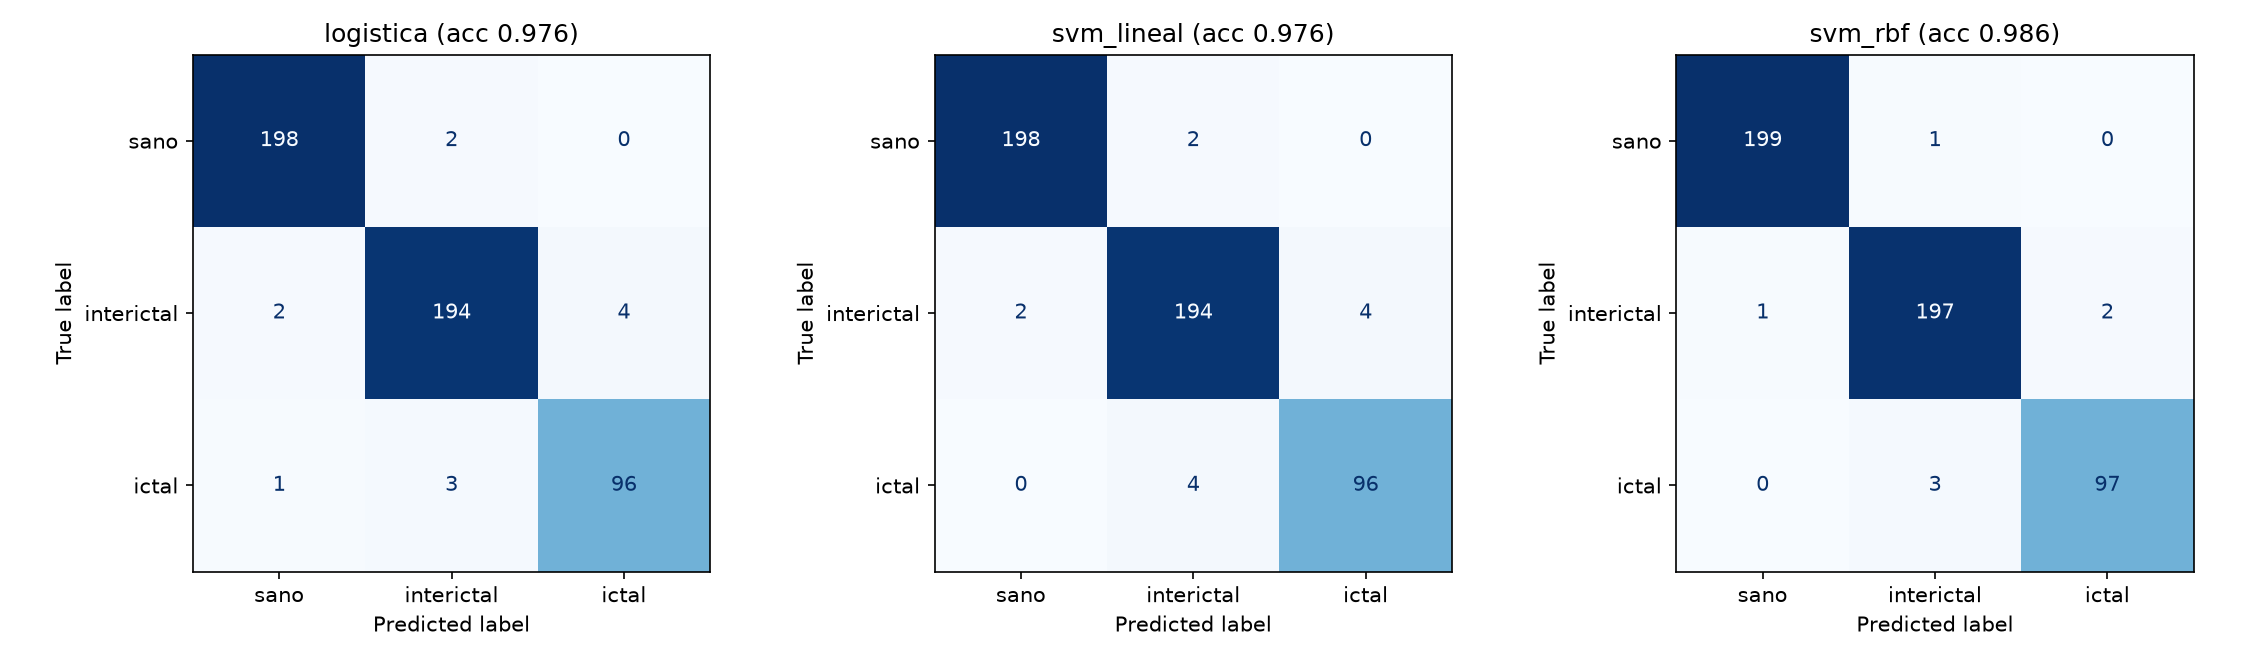
\includegraphics[width=\textwidth]{etapa3/bonn_matrices_confusion.png}
  \caption{Bonn: matrices de confusión con predicciones fuera de la partición (validación cruzada de 10 particiones).}
  \label{fig:bonn_confusion}
\end{figure}

\begin{figure}[ht]
  \centering
  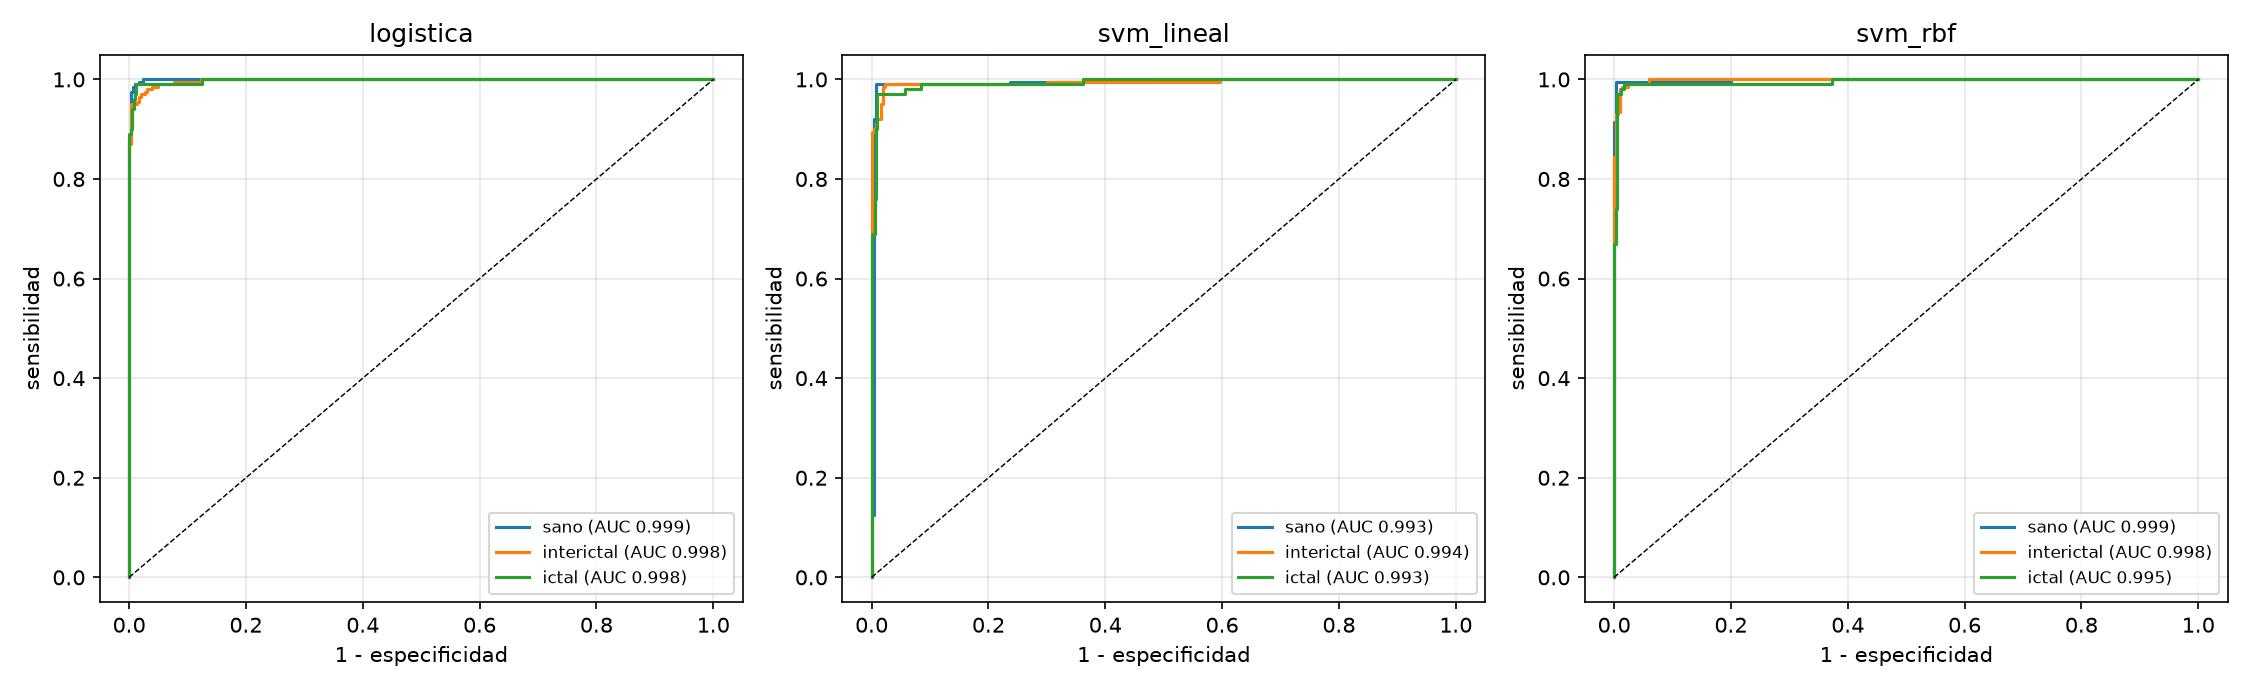
\includegraphics[width=\textwidth]{etapa3/bonn_roc.png}
  \caption{Bonn: curvas ROC de cada clase contra el resto.}
  \label{fig:bonn_roc}
\end{figure}

\subsection{Las probabilidades sobre el simplex}

Cada segmento recibe un vector $\mathbf{p} = (p_\text{sano}, p_\text{interictal}, p_\text{ictal}) \in \Delta^2$, un punto del
triángulo de la Figura~\ref{fig:simplex_teorico}. Para graficarlo en el plano se usan las coordenadas
$u = p_2 + p_3/2$, $v = \frac{\sqrt3}{2}p_3$, que llevan los vértices a $(0,0)$, $(1,0)$ y $(\frac12, \frac{\sqrt3}{2})$.

\begin{figure}[ht]
  \centering
  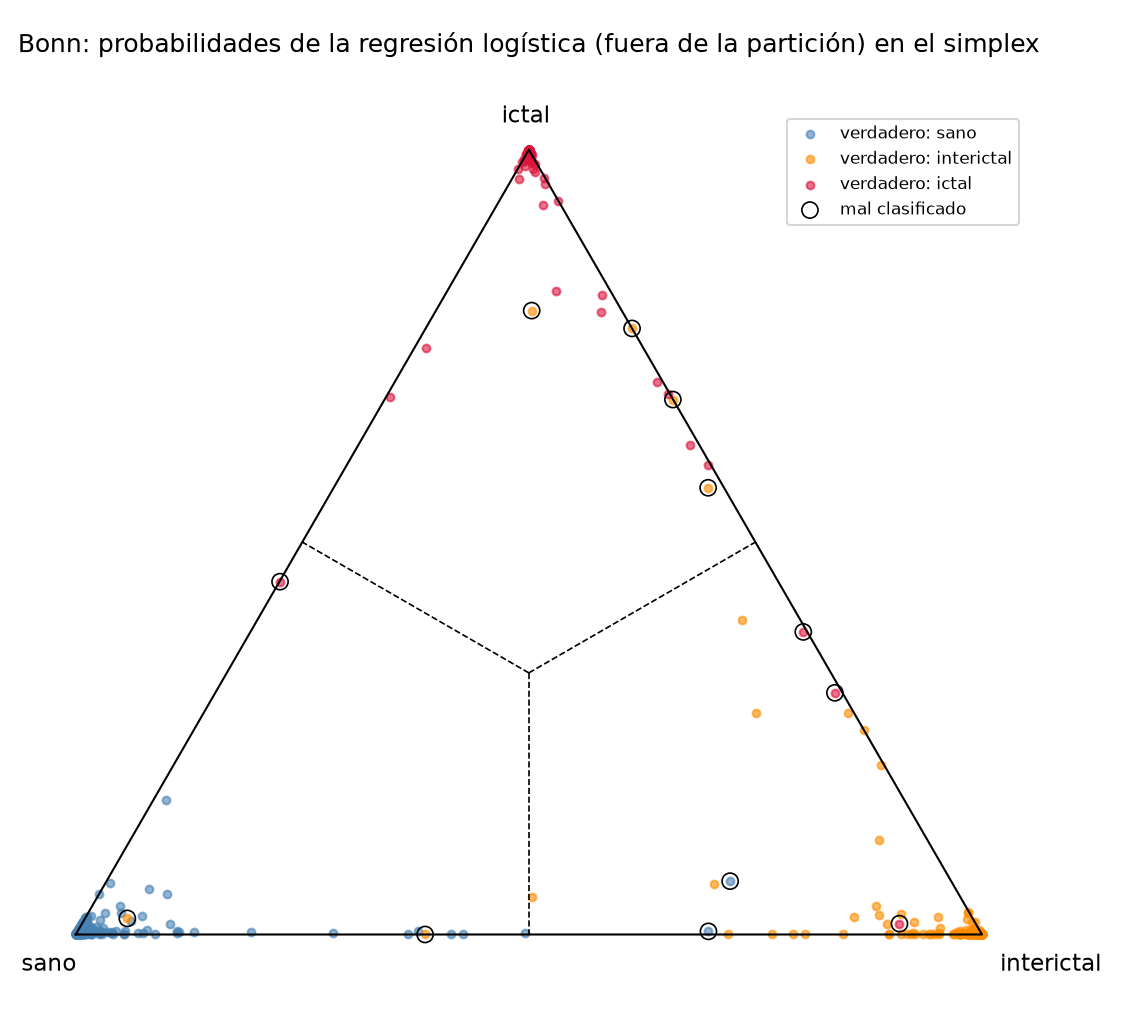
\includegraphics[width=0.75\textwidth]{etapa3/bonn_simplex.png}
  \caption{Bonn: probabilidades de la regresión logística (fuera de la partición) sobre el simplex $\Delta^2$. Las líneas
           punteadas son las fronteras de la regla $\argmax$; los círculos negros, los segmentos mal clasificados.}
  \label{fig:bonn_simplex}
\end{figure}

La Figura~\ref{fig:bonn_simplex} muestra que casi todos los segmentos quedan pegados a su vértice: el modelo predice con
mucha certeza. Los errores están sobre el lado ictal--interictal del triángulo, donde la probabilidad de ``sano'' es
casi cero: el modelo no duda entre las tres clases, duda entre dos. Algunos segmentos sanos caen sobre el lado
sano--interictal. No se verificó de qué set son; una explicación posible es la potencia alfa del set B (ojos cerrados),
que podría acercarlos a algunos registros intracraneales.

\subsection{Qué frecuencias usa el modelo}

Con atributos estandarizados, el coeficiente $w_{k,j}$ indica cuánto aumenta el puntaje de la clase $k$ si la
log-potencia de la banda $j$ sube un desvío estándar (Figura~\ref{fig:bonn_coef}).

\begin{figure}[ht]
  \centering
  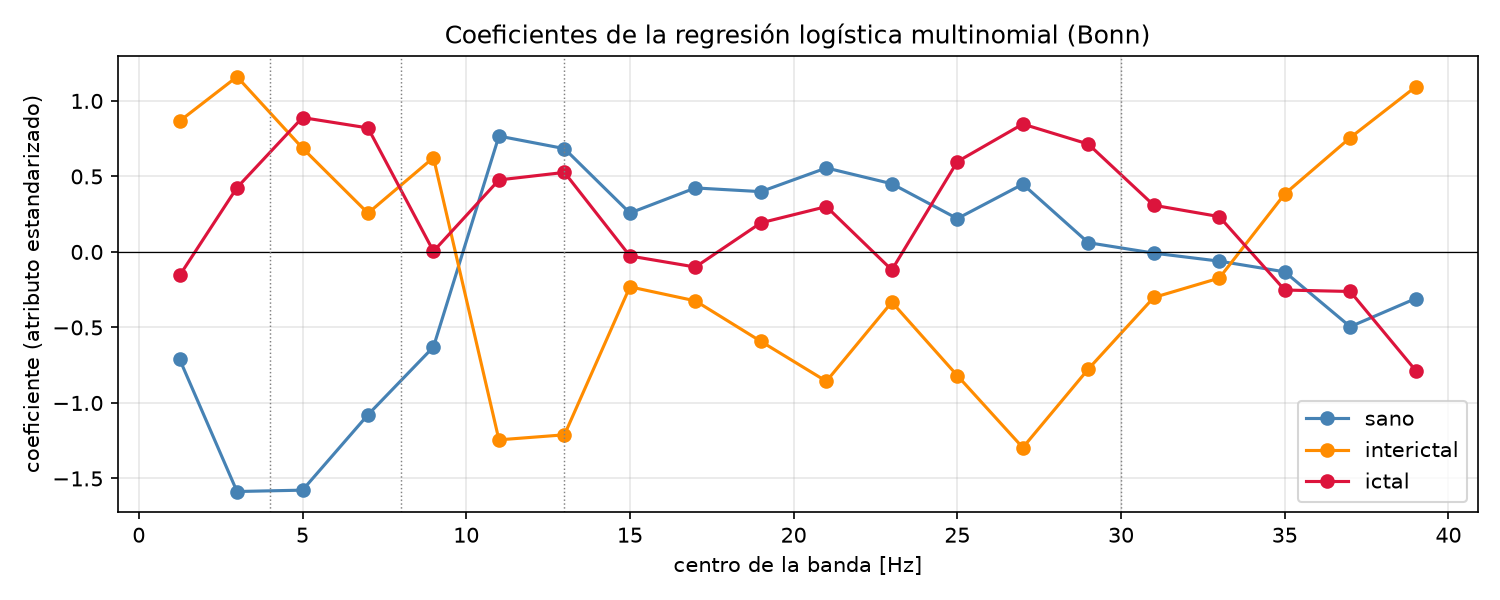
\includegraphics[width=0.9\textwidth]{etapa3/bonn_coeficientes.png}
  \caption{Coeficientes de la regresión logística multinomial en Bonn, por banda de 2~Hz. Las líneas verticales marcan
           los límites de las bandas clínicas (4, 8, 13 y 30~Hz).}
  \label{fig:bonn_coef}
\end{figure}

\begin{itemize}
  \item \textbf{Sano:} coeficientes negativos grandes entre 2 y 8~Hz ($-1{,}6$) y positivos entre 10 y 30~Hz. El EEG de
        superficie de voluntarios sanos tiene relativamente poca actividad lenta y más alfa y beta.
  \item \textbf{Interictal:} el patrón opuesto: positivo en delta (hasta $+1{,}2$ en 2--4~Hz) y negativo en alfa y beta.
        Coincide con la Tabla~\ref{tab:bonn_bandas}, donde los sets C y D tienen 60--67~\% de su potencia en delta.
        También es positivo entre 36 y 40~Hz, probablemente por diferencias del equipo intracraneal.
  \item \textbf{Ictal:} positivo en theta (4--8~Hz, $+0{,}9$), donde está la descarga rítmica, y en beta alta (24--30~Hz).
\end{itemize}
Como softmax es invariante a sumar el mismo vector a los tres $\vw_k$, solo importan las diferencias entre clases: los
coeficientes individuales se interpretan con cuidado.

\section{Verificación de la optimalidad global}
\label{sec:verif_optimalidad}

\subsection{Regresión logística: 20 puntos iniciales, un solo óptimo}

Se toma el problema binario ictal contra el resto en Bonn, con 20 atributos estandarizados más el sesgo y $\lambda = 0{,}01$,
y se implementa el descenso por gradiente a mano con el gradiente~\eqref{eq:hess_logistica} y el paso $\eta = 1/L$ de
la cota~\eqref{eq:L_logistica}: $L = 4{,}298$, $\eta = 0{,}233$. Se corren 20\,000 iteraciones desde 20 puntos
iniciales $\vth_0 \sim \mathcal{N}(\mathbf{0}, 9I)$, que quedan a una distancia media de 13,2 del óptimo. Como
referencia se usa la solución de \texttt{scikit-learn} con tolerancia $10^{-12}$, de valor $J^* = 0{,}07699786$.

Resultados:
\begin{itemize}
  \item Los 20 valores finales de $J$ coinciden con $J^*$ en las 8 cifras informadas.
  \item La mayor distancia entre un $\vth$ final y el de referencia es $3{,}0\times10^{-7}$.
  \item La brecha $J(\vth_k) - J^*$ cae en línea recta en escala logarítmica (Figura~\ref{fig:optimalidad}, izquierda):
        convergencia lineal, como predice el Teorema~\ref{teo:convergencia}. La curva se aplana en $10^{-16}$, la
        precisión del punto flotante de doble precisión.
\end{itemize}
La pendiente observada concuerda con la teoría. En el óptimo, el menor autovalor de la Hessiana es $\mu \approx 0{,}0081$,
lo que da $\kappa = L/\mu \approx 528$ y una tasa de $1 - 1/\kappa \approx 0{,}998$ por iteración: unas 14\,600
iteraciones para 12 órdenes de magnitud, dentro de las 20\,000 usadas. El $\kappa$ alto se debe a que $L$ es una cota
global (supone $p_i(1 - p_i) = \frac14$) mientras que cerca del óptimo casi todos los $p_i$ están cerca de 0 o 1 y la
curvatura real es mucho menor: el mayor autovalor de la Hessiana en el óptimo es 0,24, no 4,3.

\begin{figure}[ht]
  \centering
  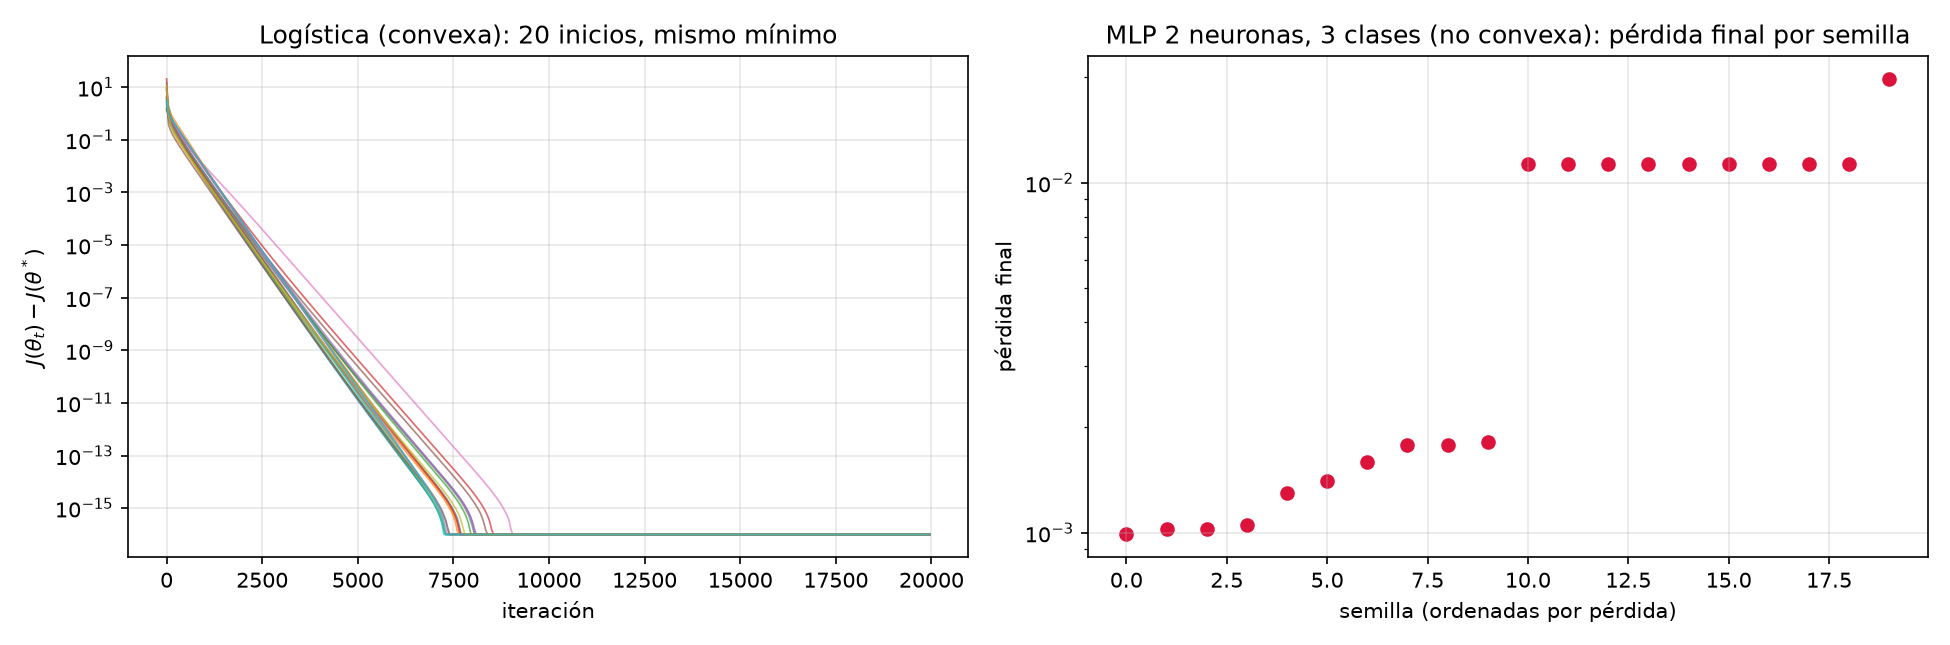
\includegraphics[width=\textwidth]{etapa3/optimalidad_convexo_vs_no_convexo.png}
  \caption{Izquierda: brecha $J(\vth_k) - J^*$ de la regresión logística (convexa) desde 20 puntos iniciales, en escala
           logarítmica. Derecha: pérdida final de un perceptrón de 2 neuronas (no convexo) con 20 semillas, ordenadas.}
  \label{fig:optimalidad}
\end{figure}

\subsection{Contraste: una red neuronal chica}

Se entrena un perceptrón multicapa con una capa oculta $\tanh$ hasta convergencia (L-BFGS, tolerancia $10^{-10}$) desde
20 semillas, en dos configuraciones.

\paragraph{(a) Ictal contra el resto, 4 neuronas, penalización $\alpha = 1$.} Las 20 semillas terminan con la \emph{misma}
pérdida, 0,041217, pero con pesos distintos: las soluciones de las semillas 6 y 14 están a distancia 9,7. En el punto
medio entre ambas, la pérdida es \textbf{0,596}, catorce veces mayor. Por el Teorema~\ref{teo:local_global}(2) eso es
imposible si la función es convexa. Son mínimos equivalentes por las simetrías de la Sección~\ref{sec:no_convexo}
(permutación de neuronas y cambios de signo), que en una función convexa no pueden existir.

\paragraph{(b) Tres clases, 2 neuronas, $\alpha = 10^{-3}$.} Aparecen \textbf{8 valores distintos} de la pérdida final, entre
0,00099 y 0,01983: un factor 20 (Figura~\ref{fig:optimalidad}, derecha). Nueve de las 20 semillas quedan en el mismo
mínimo local, con pérdida 0,01135, unas diez veces peor que el mejor. Son mínimos locales genuinos: con solo 2
neuronas, la red no puede representar bien las tres clases desde cualquier configuración inicial, y el optimizador
queda atrapado en la que le toca.

\paragraph{Consecuencia.} En un modelo convexo, una corrida alcanza. En una red neuronal el resultado depende de la
semilla, y comparar dos optimizadores con una corrida de cada uno no permite separar el efecto del optimizador del
azar de la inicialización. Por eso en el Capítulo~\ref{cap:cnn} cada configuración se corre con 5 semillas.

\section{Verificación de KKT en el SVM}
\label{sec:verif_kkt}

Se entrena un SVM lineal con $C = 1$ para separar el set E (ictal, $y = +1$) del set D (interictal del foco, $y = -1$):
200 segmentos, 20 atributos estandarizados, tolerancia $10^{-8}$. A partir de los $\alpha_i$ que devuelve el
solucionador se verifica cada condición de la Sección~\ref{sec:svm_dual} (Tabla~\ref{tab:kkt_verif}).

\begin{table}[ht]
\centering
\caption{Verificación numérica de las condiciones KKT del SVM lineal (Bonn, E contra D, $C = 1$). $m_i = y_i f(\vx_i)$.}
\label{tab:kkt_verif}
\begin{tabular}{lll}
\toprule
Condición & Teoría & Medido \\
\midrule
Estacionariedad en $\vw$ & $\vw = \sum_i\alpha_i y_i\vx_i$ & diferencia máxima $0{,}0$ \\
Estacionariedad en $b$ & $\sum_i\alpha_i y_i = 0$ & $-1{,}1\times10^{-15}$ \\
Factibilidad dual & $0 \le \alpha_i \le C$ & $\min = 0$, $\max = 1$ \\
$\alpha_i = 0$ & $m_i \ge 1$ & 180 puntos, $\min m_i = 1{,}0127$ \\
$0 < \alpha_i < C$ & $m_i = 1$ & 9 puntos, $m_i \in [1{,}0000;\ 1{,}0000]$ \\
$\alpha_i = C$ & $m_i \le 1$ & 11 puntos, $\max m_i = 0{,}6293$ \\
Valor primal & & 11,692841 \\
Valor dual & & 11,692839 \\
Brecha relativa & $0$ (Slater) & $1{,}55\times10^{-7}$ \\
\bottomrule
\end{tabular}
\end{table}

\begin{figure}[ht]
  \centering
  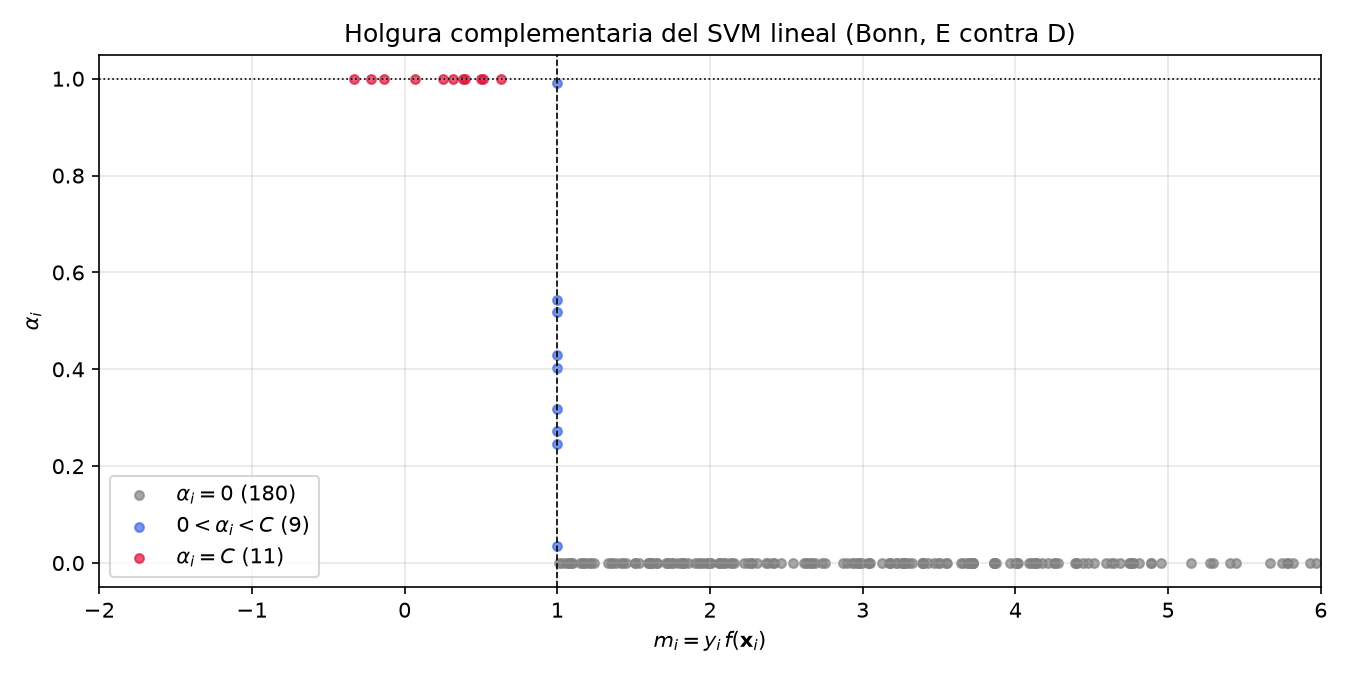
\includegraphics[width=0.85\textwidth]{etapa3/svm_kkt.png}
  \caption{Holgura complementaria en el SVM lineal: multiplicador $\alpha_i$ contra margen funcional $m_i$. Los puntos con
           $\alpha_i = 0$ están a la derecha de $m = 1$; los libres, sobre $m = 1$; los acotados en $C$, a la izquierda.}
  \label{fig:svm_kkt}
\end{figure}

Todas las condiciones se cumplen a la precisión numérica. La Figura~\ref{fig:svm_kkt} muestra la holgura complementaria:
ningún punto está en las zonas prohibidas ($\alpha_i > 0$ con $m_i > 1$, o $\alpha_i < C$ con $m_i < 1$). De los 200
segmentos solo 20 tienen $\alpha_i > 0$: el hiperplano queda determinado por esos 20 vectores soporte, y los otros 180
se podrían borrar sin que cambie la solución. De los 20, 11 están dentro del margen o mal clasificados
($\alpha_i = C$). La brecha entre primal y dual es del orden de la tolerancia del solucionador: hay dualidad fuerte,
como garantiza la condición de Slater.

\section{Resultados en CHB-MIT: paciente nuevo (LOPO)}
\label{sec:lopo}

\subsection{Resumen}

La Tabla~\ref{tab:lopo_resumen} resume los resultados de dejar un paciente fuera, sumando las 34 crisis de los 6
pacientes de prueba. Se comparan dos variantes de atributos (\emph{global}: sin calibrar; \emph{calibrado}: restando la
mediana del paciente, Sección~\ref{sec:calibracion}) y dos reglas de umbral (cero, que corresponde a $p = 0{,}5$ con
clases balanceadas, y Neyman-Pearson con $\alpha = 10^{-3}$).

\begin{table}[ht]
\centering
\caption{CHB-MIT, dejar un paciente fuera. AUC: media entre los 6 pacientes. Sensibilidad y especificidad por ventana:
media entre pacientes. Crisis y FA/h: totales sobre los 6 pacientes. Latencia: mediana.}
\label{tab:lopo_resumen}
\small
\begin{tabular}{lllccccccc}
\toprule
Variante & Modelo & Umbral & AUC & Sens. & Espec. & Crisis & FA/h & Lat. [s] \\
\midrule
\multirow{4}{*}{global}
 & logística & cero & 0,946 & 0,627 & 0,893 & 28/34 & 17,13 & 12,3 \\
 & logística & NP   & 0,946 & 0,363 & 0,994 & 23/34 & 2,10  & 20,0 \\
 & SVM lineal & cero & 0,944 & 0,625 & 0,890 & 28/34 & 17,23 & 12,3 \\
 & SVM lineal & NP   & 0,944 & 0,352 & 0,994 & 24/34 & 2,18  & 20,0 \\
\midrule
\multirow{4}{*}{calibrado}
 & logística & cero & 0,949 & 0,779 & 0,955 & 34/34 & 11,00 & 12,5 \\
 & logística & NP   & 0,949 & 0,334 & 0,994 & 24/34 & \textbf{1,14} & 25,3 \\
 & SVM lineal & cero & 0,948 & 0,772 & 0,953 & 34/34 & 11,30 & 12,5 \\
 & SVM lineal & NP   & 0,948 & 0,334 & 0,994 & 24/34 & 1,20  & 22,3 \\
\bottomrule
\end{tabular}
\end{table}

\paragraph{El umbral natural no sirve.} Con umbral cero y atributos calibrados se detectan las 34 crisis, pero con 11
falsas alarmas por hora: más de 250 por día. La especificidad por ventana de 0,955 parece alta, pero con 900 ventanas
por hora el 4,5~\% restante son 40 ventanas falsas por hora. Es la ilustración directa de la
Sección~\ref{sec:zona_util}.

\paragraph{Neyman-Pearson.} Con $\alpha = 10^{-3}$ las falsas alarmas bajan diez veces, a 1,1--2,2 por hora, a cambio de
detectar el 70~\% de las crisis y de duplicar la latencia. Es el compromiso sensibilidad--especificidad resuelto
explícitamente con un multiplicador de Lagrange.

\paragraph{Calibrar.} Con la misma sensibilidad por evento (24/34), restar la mediana del paciente baja las falsas alarmas
casi a la mitad (de 2,10 a 1,14 por hora con la logística). Confirma que buena parte de la dificultad de generalizar a un
paciente nuevo es la diferencia de nivel basal, el término $2\log g_{p,c}$ del modelo.

\paragraph{Logística contra SVM.} Los resultados son casi idénticos. Ambos son clasificadores lineales sobre los mismos
atributos; solo cambia la pérdida (logística contra bisagra), y con miles de ejemplos la frontera resultante es muy
parecida.

\subsection{Por paciente}

\begin{table}[ht]
\centering
\caption{CHB-MIT, LOPO, regresión logística con umbral de Neyman-Pearson, por paciente de prueba.}
\label{tab:lopo_pacientes}
\begin{tabular}{lcccccc}
\toprule
 & \multicolumn{3}{c}{global} & \multicolumn{3}{c}{calibrado} \\
\cmidrule(lr){2-4}\cmidrule(lr){5-7}
Paciente & AUC & Crisis & FA/h & AUC & Crisis & FA/h \\
\midrule
chb01 & 0,971 & 2/7 & 0,10 & 0,982 & 3/7 & 0,00 \\
chb02 & 0,956 & 1/3 & 1,22 & 0,978 & 1/3 & 0,09 \\
chb03 & 0,949 & 3/7 & 1,90 & 0,943 & 4/7 & 4,59 \\
chb05 & 0,980 & 5/5 & 2,65 & 0,983 & 5/5 & 0,00 \\
chb08 & 0,835 & 5/5 & 1,98 & 0,831 & 5/5 & 0,20 \\
chb10 & 0,986 & 7/7 & 4,11 & 0,978 & 6/7 & 1,46 \\
\bottomrule
\end{tabular}
\end{table}

La Tabla~\ref{tab:lopo_pacientes} muestra que \textbf{la restricción de Neyman-Pearson no se cumple igual en todos los
pacientes}: el umbral se fija con los cinco de entrenamiento y en el paciente nuevo las falsas alarmas van de 0 a 4,6 por
hora. Es la advertencia de la Observación~\ref{obs:np_supuesto}: el lema supone que la distribución del puntaje sin crisis
es la misma en la calibración y en el uso, y entre pacientes eso no vale. La calibración la acerca en cinco pacientes,
pero en chb03 la empeora (de 1,90 a 4,59 FA/h).

\begin{figure}[ht]
  \centering
  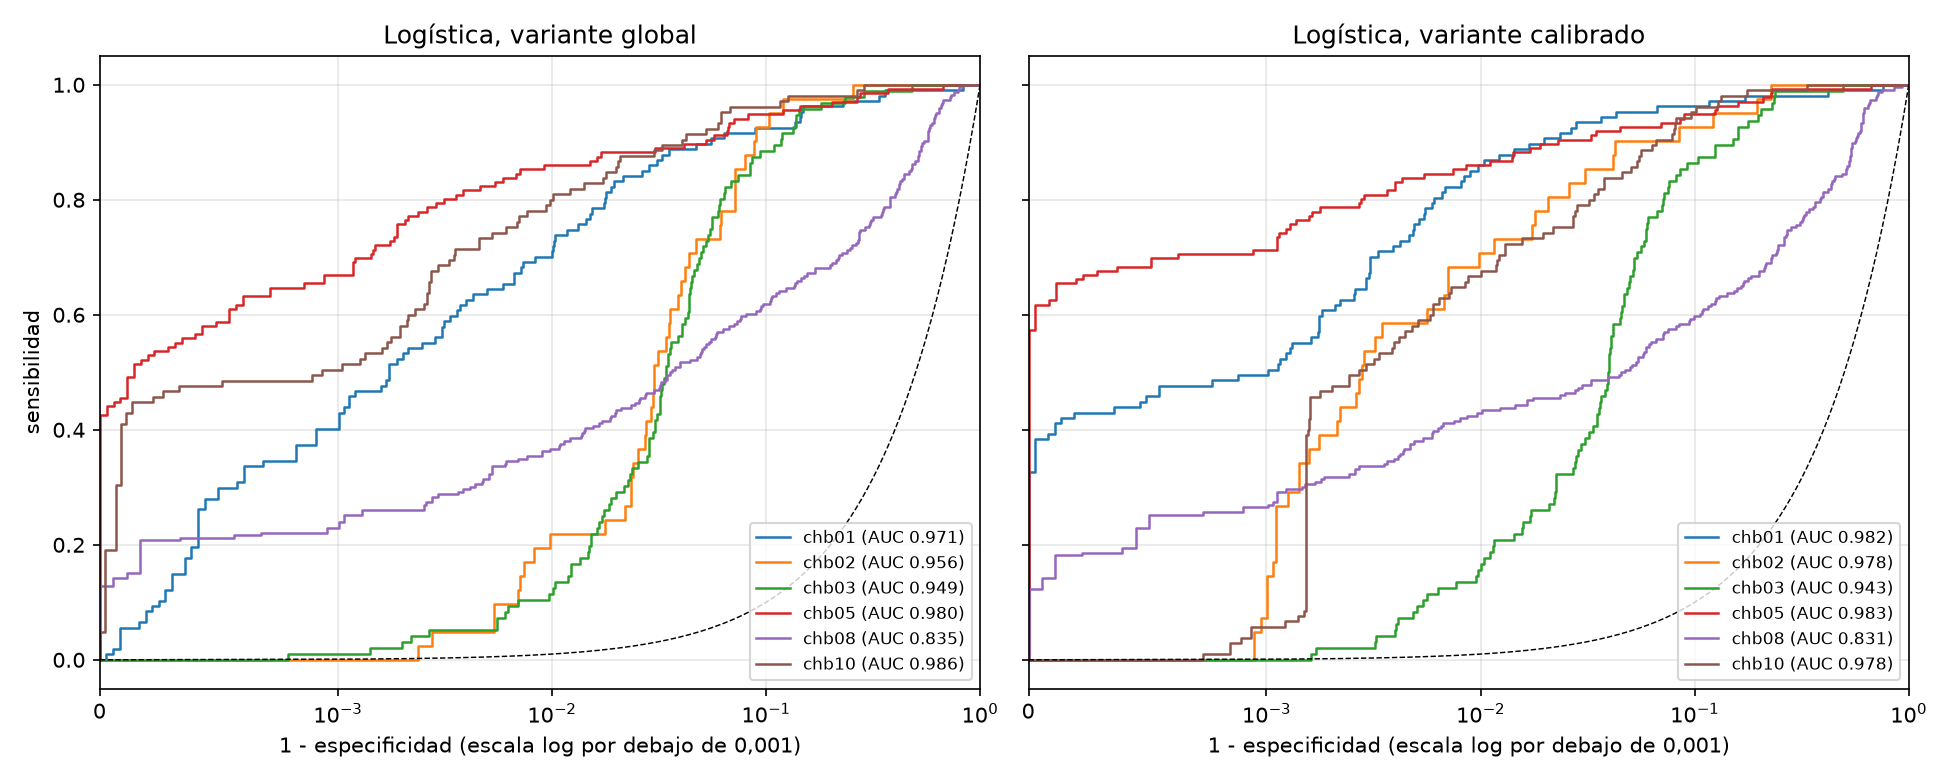
\includegraphics[width=\textwidth]{etapa3/chbmit_lopo_roc.png}
  \caption{CHB-MIT, LOPO: curvas ROC de la regresión logística por paciente de prueba, sin calibrar (izquierda) y
           calibrada (derecha). Eje horizontal lineal entre 0 y $10^{-3}$ y logarítmico por encima.}
  \label{fig:lopo_roc}
\end{figure}

Las curvas ROC por paciente (Figura~\ref{fig:lopo_roc}) muestran por qué el AUC no alcanza:
\begin{itemize}
  \item \textbf{chb03} tiene AUC 0,95, pero con menos de 1~\% de falsos positivos casi no detecta nada: sus ventanas con
        mayor puntaje no son crisis. Es el paciente más difícil en la zona útil, también para la CNN.
  \item \textbf{chb05 y chb10} detectan la mitad de las ventanas ictales con menos de 0,1~\% de falsos positivos.
  \item \textbf{chb08} tiene el menor AUC (0,83): sus crisis son las más largas y las de menor aumento de potencia
        (Tabla~\ref{tab:dif_log}). Aun así, se detectan sus 5 crisis, porque al ser largas basta con acertar algunas
        ventanas de cada una.
  \item \textbf{Calibrar} mejora mucho la zona de baja tasa de falsos positivos en chb01 y chb05.
\end{itemize}

\begin{figure}[ht]
  \centering
  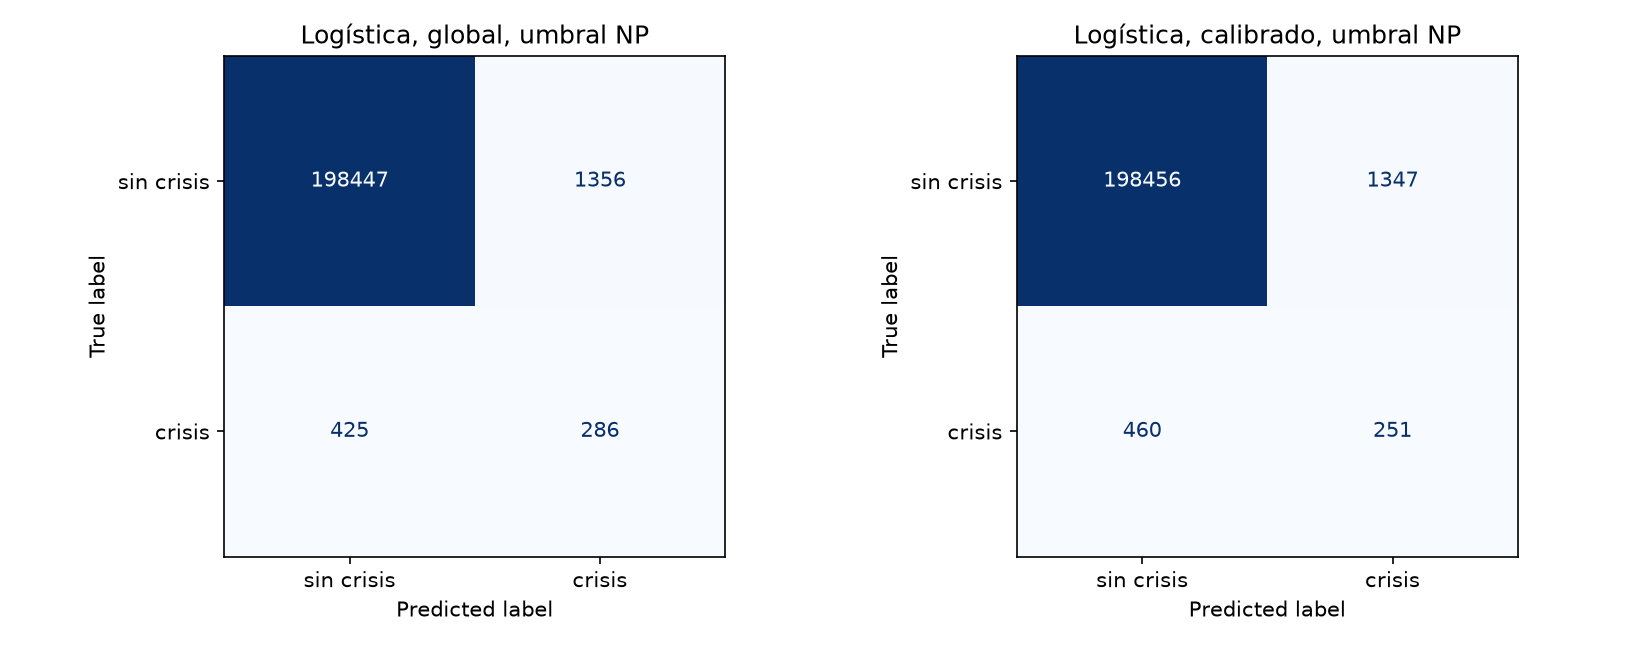
\includegraphics[width=0.85\textwidth]{etapa3/chbmit_lopo_confusion.png}
  \caption{CHB-MIT, LOPO: matrices de confusión por ventana sumadas sobre los 6 pacientes de prueba (regresión logística,
           umbral de Neyman-Pearson, sin ventanas de borde).}
  \label{fig:lopo_confusion}
\end{figure}

La matriz de confusión agregada de la variante calibrada (Figura~\ref{fig:lopo_confusion}) tiene 251 verdaderos positivos,
460 falsos negativos, 1347 falsos positivos y 198\,456 verdaderos negativos. Hay más falsos positivos que ventanas ictales
en total: por~\eqref{eq:vpp_bayes}, el VPP por ventana es apenas $251/1598 = 0{,}16$. Por evento el panorama es mejor,
porque los falsos positivos se agrupan en rachas y las crisis duran varias ventanas.

\section{Resultados en CHB-MIT: partición fija}
\label{sec:fija_convexos}

Para comparar con la CNN, los modelos convexos se evalúan también con la partición fija de la Tabla~\ref{tab:particion}:
entrenamiento con chb02, chb05 y chb08, umbral de Neyman-Pearson calculado con las ventanas sin crisis de chb01, y prueba
en chb03 y chb10.

\begin{table}[ht]
\centering
\caption{CHB-MIT, partición fija. Prueba: chb03 y chb10 (14 crisis, 87,8 horas sin crisis).}
\label{tab:fija_convexos}
\begin{tabular}{llcccccc}
\toprule
Variante & Modelo & AUC val. & AUC prueba & Sens. & Crisis & FA/h & Lat. [s] \\
\midrule
global    & logística  & 0,969 & 0,799 & 0,304 & 5/14 & 3,26 & 14,0 \\
global    & SVM lineal & 0,967 & 0,798 & 0,304 & 7/14 & 2,94 & 18,0 \\
calibrado & logística  & 0,979 & \textbf{0,934} & 0,269 & 7/14 & 1,22 & 26,0 \\
calibrado & SVM lineal & 0,977 & 0,930 & 0,244 & 6/14 & \textbf{1,00} & 24,5 \\
\bottomrule
\end{tabular}
\end{table}

Con solo tres pacientes de entrenamiento, la variante global generaliza mal: AUC de 0,97 en validación pero 0,80 en
prueba. La calibrada llega a 0,93 en prueba y reduce las falsas alarmas de 3,3 a 1,2 por hora (Tabla~\ref{tab:fija_convexos}).
Detecta la mitad de las crisis, con una latencia mediana de 26~s. La regresión logística calibrada es la línea de base contra
la que se compara la CNN en el Capítulo~\ref{cap:resultados}.

\chapter{Red convolucional y optimizadores}
\label{cap:cnn}

Los modelos convexos del Capítulo~\ref{cap:convexos} trabajan con 90 números por ventana: la potencia de cada canal
en cinco bandas fijas. Una red convolucional (CNN) puede trabajar directamente con el espectrograma completo y aprender
qué patrones de frecuencia y tiempo indican una crisis. El precio es que su entrenamiento deja de ser un problema convexo
(Sección~\ref{sec:no_convexo}): el resultado depende del punto inicial, del algoritmo de optimización y de la tasa de
aprendizaje. Este capítulo describe la red, deduce cómo se calcula su gradiente, presenta los seis optimizadores que se
comparan y detalla el diseño del experimento. Los resultados están en el Capítulo~\ref{cap:resultados}. El código es
\texttt{scripts/entrenar\_cnn.py} y el análisis, \texttt{etapa4\_cnn\_optimizadores.ipynb}.

\section{Entrada}
\label{sec:cnn_entrada}

Cada ventana de 4~s se representa con el tensor que se guardó en el preprocesamiento (Sección~\ref{sec:preproc}):
\begin{equation}
  \mathbf{X} \in \R^{18 \times 40 \times 7}, \qquad
  X_{c,f,t} = \log_{10}\big|\mathrm{STFT}\{x_c\}(f, t)\big|^2,
\end{equation}
con 18 canales bipolares $c$, 40 frecuencias $f$ de 1 a 40~Hz (resolución de 1~Hz, ventana de Hann de 1~s) y 7 cuadros de
tiempo $t$ (salto de 0,5~s). Antes de entrar a la red se aplican dos transformaciones:
\begin{enumerate}
  \item \textbf{Calibración por paciente} (ecuación~\eqref{eq:calibracion}): a cada canal y frecuencia se le resta la mediana de
        ese paciente sobre todas sus ventanas y cuadros. Elimina el término $2\log g_{p,c}$ del modelo~\eqref{eq:modelo_eeg}
        y, además, la forma espectral basal propia de cada paciente.
  \item \textbf{Estandarización}: a cada canal y frecuencia se le resta la media y se lo divide por el desvío, calculados
        solo con el conjunto de entrenamiento.
\end{enumerate}
Los canales del EEG se tratan como los \emph{canales de entrada} de la convolución (igual que los tres colores de una
imagen), y el plano frecuencia--tiempo, como la ``imagen''. Así cada filtro de la primera capa combina los 18 canales
con pesos propios, y se desplaza a lo largo de la frecuencia y del tiempo.

\section{Arquitectura}
\label{sec:arquitectura}

\subsection{Capas}

\paragraph{Convolución.} Una capa convolucional con $C_\text{in}$ canales de entrada, $C_\text{out}$ de salida y núcleo de
$k_f \times k_t$ calcula
\begin{equation}
  Z_{o,f,t} = b_o + \sum_{c=1}^{C_\text{in}}\ \sum_{i=1}^{k_f}\ \sum_{j=1}^{k_t} W_{o,c,i,j}\; X_{c,\ f + i - r_f,\ t + j - r_t},
  \qquad r_f = \tfrac{k_f + 1}{2},\ r_t = \tfrac{k_t + 1}{2},
  \label{eq:conv}
\end{equation}
con relleno de ceros en los bordes para que la salida tenga el mismo tamaño que la entrada. Estrictamente es una
\emph{correlación cruzada} (la convolución del Capítulo~\ref{cap:fourier} invierte el núcleo), pero como $W$ se aprende la
diferencia es irrelevante. Tiene $C_\text{out}(C_\text{in}k_fk_t + 1)$ parámetros, independientemente del tamaño de la entrada:
los mismos pesos se usan en todas las posiciones.

Esa repetición de pesos da la propiedad que motiva la arquitectura: la capa es \textbf{equivariante a traslaciones}. Si la
entrada se desplaza $\Delta$ posiciones a lo largo de la frecuencia, la salida se desplaza igual. Una descarga rítmica con
fundamental $f_0$ (ecuación~\eqref{eq:descarga}) aparece como una línea horizontal en el espectrograma; si en otro paciente
$f_0$ es distinta, la línea está más arriba o más abajo, y el mismo filtro la detecta. Es la variabilidad entre pacientes que
mostró la Tabla~\ref{tab:dif_log}. (Como el eje de frecuencias es lineal, los armónicos $2f_0, 3f_0$ no se desplazan lo mismo
que la fundamental, así que la equivariancia es solo aproximada para el patrón completo.)

\paragraph{Normalización por lotes \parencite{ioffe2015}.} Para cada canal $o$, sobre las $B$ ventanas del lote y todas
las posiciones $(f, t)$, se calcula la media $\mu_o$ y la varianza $\sigma_o^2$, y
\begin{equation}
  \hat Z_{o,f,t} = \frac{Z_{o,f,t} - \mu_o}{\sqrt{\sigma_o^2 + \epsilon}}, \qquad
  \text{BN}(Z)_{o,f,t} = \gamma_o\,\hat Z_{o,f,t} + \beta_o,
  \label{eq:bn}
\end{equation}
con $\gamma_o, \beta_o$ aprendidos y $\epsilon = 10^{-5}$. Durante la evaluación no hay lote: se usan promedios móviles de
$\mu_o$ y $\sigma_o^2$ acumulados en el entrenamiento (factor 0,1 por paso). Su efecto sobre la optimización se analiza en la
Sección~\ref{sec:bn_escala}.

\paragraph{ReLU} $\max(0, z)$, elemento a elemento. \textbf{Max pooling} $(2,1)$: toma el máximo de cada par de frecuencias
vecinas, reduciendo a la mitad el eje de frecuencia y dejando el tiempo igual. \textbf{Promedio global}: promedia cada
canal sobre todas las posiciones, dejando un vector de 64 números. \textbf{Dropout} \parencite{goodfellow2016}: durante el
entrenamiento pone en cero cada componente con probabilidad $p = 0{,}3$ y multiplica las restantes por $1/(1-p)$, de modo que
la esperanza no cambia; en evaluación no hace nada. Finalmente una capa lineal da un único número, el \emph{logit} $z$.

\subsection{Tabla de capas}

\begin{table}[ht]
\centering
\caption{Arquitectura de la CNN. Entrada: $18 \times 40 \times 7$ (canales $\times$ frecuencias $\times$ cuadros de tiempo).
Los parámetros incluyen pesos, sesgos y los $\gamma, \beta$ de la normalización por lotes.}
\label{tab:cnn_capas}
\begin{tabular}{clcr}
\toprule
\# & Bloque & Salida & Parámetros \\
\midrule
1 & Conv $5\times3$, 32 filtros + BN + ReLU + MaxPool $(2,1)$ & $32 \times 20 \times 7$ & 8\,736 \\
2 & Conv $3\times3$, 64 filtros + BN + ReLU + MaxPool $(2,1)$ & $64 \times 10 \times 7$ & 18\,624 \\
3 & Conv $3\times3$, 64 filtros + BN + ReLU                   & $64 \times 10 \times 7$ & 37\,056 \\
4 & Promedio global + Dropout 0,3 + Lineal                    & 1 (logit)               & 65 \\
\midrule
  & Total &  & 64\,481 \\
\bottomrule
\end{tabular}
\end{table}

Por ejemplo, el bloque 1 tiene $32\cdot(18\cdot5\cdot3 + 1) = 8\,672$ parámetros de convolución y $2\cdot32 = 64$ de la
normalización. El primer núcleo es más alto en frecuencia ($5$) que en tiempo ($3$) para captar picos espectrales de
algunos hertz de ancho.

\paragraph{Campo receptivo.} Cada salida de la última capa convolucional depende de una región de la entrada que se calcula
capa por capa: un núcleo de tamaño $k$ agrega $(k-1)\cdot s$ posiciones, donde $s$ es el producto de los pasos de los
\emph{poolings} anteriores. En frecuencia: $5 \to 6 \to 10 \to 12 \to 20$, es decir 20~Hz. En tiempo: $3 \to 5 \to 7$
cuadros, la ventana entera. Cada neurona de la última capa ve la mitad del rango de frecuencias y los 4~s completos, y el
promedio global combina todas.

\paragraph{Tamaño.} 64\,481 parámetros es poco para una CNN, y es deliberado: hay solo 403 ventanas ictales de
entrenamiento (13 crisis de 3 pacientes), y una red más grande las memorizaría. Para comparar, la regresión logística de
CHB-MIT tiene 91 parámetros.

\subsection{Salida y pérdida}

La salida $z = f_{\vth}(\mathbf{X})$ se interpreta como el logit de la probabilidad de crisis, $\hat p = \sigma(z)$, y la red
se entrena minimizando la entropía cruzada binaria promedio sobre el lote $\mathcal{B}$:
\begin{equation}
  J_{\mathcal{B}}(\vth) = \frac{1}{|\mathcal{B}|}\sum_{i \in \mathcal{B}} \ell(z_i, y_i), \qquad
  \ell(z, y) = -y\log\sigma(z) - (1 - y)\log\big(1 - \sigma(z)\big).
  \label{eq:bce}
\end{equation}
Es la pérdida~\eqref{eq:logistica_binaria} de la regresión logística, con la diferencia de que $z$ ya no es lineal en $\vth$.
Por eso es convexa en $z$ pero no en $\vth$. Numéricamente se calcula como
$\ell = \max(z, 0) - zy + \log(1 + e^{-|z|})$, que no desborda para $|z|$ grande (función
\texttt{binary\_cross\_entropy\_with\_logits}). Como la decisión final usa un umbral de Neyman-Pearson sobre $z$
(Sección~\ref{sec:umbral_np}), la calibración de $\hat p$ como probabilidad no importa, solo el orden de los puntajes.

\section{Retropropagación}
\label{sec:retropropagacion}

Todos los optimizadores de este capítulo necesitan el gradiente $\nabla_{\vth}J_{\mathcal{B}}$. La red es una composición
de funciones, $z = h_L \circ h_{L-1} \circ \cdots \circ h_1(\mathbf{X})$, cada una con sus parámetros $\vth_\ell$. La
\textbf{retropropagación} es la regla de la cadena aplicada de la salida hacia la entrada, reutilizando los resultados
intermedios.

\paragraph{Último paso.} Con $\sigma'(z) = \sigma(z)(1 - \sigma(z))$,
\begin{equation}
  \frac{\partial\ell}{\partial z} = -y\,\frac{\sigma(z)(1 - \sigma(z))}{\sigma(z)} + (1 - y)\,\frac{\sigma(z)(1 - \sigma(z))}{1 - \sigma(z)}
  = \sigma(z) - y = \hat p - y.
  \label{eq:grad_bce}
\end{equation}
Es el caso binario de~\eqref{eq:grad_ce}: \emph{predicción menos verdad}. El gradiente es grande cuando la red se equivoca
con confianza y casi cero cuando acierta con confianza: las ventanas fáciles casi no aportan al aprendizaje.

\paragraph{Recursión.} Sea $\mathbf{a}_\ell = h_\ell(\mathbf{a}_{\ell-1}; \vth_\ell)$ la salida de la capa $\ell$ y
$\boldsymbol\delta_\ell = \partial\ell/\partial\mathbf{a}_\ell$ (el ``error'' que llega a esa capa). Partiendo de
$\delta_L = \hat p - y$,
\begin{equation}
  \frac{\partial\ell}{\partial\vth_\ell} = \Big(\frac{\partial\mathbf{a}_\ell}{\partial\vth_\ell}\Big)^{\!\top}\boldsymbol\delta_\ell,
  \qquad
  \boldsymbol\delta_{\ell-1} = \Big(\frac{\partial\mathbf{a}_\ell}{\partial\mathbf{a}_{\ell-1}}\Big)^{\!\top}\boldsymbol\delta_\ell.
  \label{eq:backprop}
\end{equation}
Nunca se forman las matrices jacobianas: cada capa sabe calcular directamente el producto de su jacobiana transpuesta por un
vector. Para las capas usadas:
\begin{itemize}
  \item \textbf{Lineal} $z = \vw^\top\mathbf{a} + b$: $\partial\ell/\partial\vw = \delta\,\mathbf{a}$, $\partial\ell/\partial b = \delta$,
        $\boldsymbol\delta_\text{entrada} = \delta\,\vw$.
  \item \textbf{Convolución}~\eqref{eq:conv}: derivando,
        \[
          \frac{\partial\ell}{\partial W_{o,c,i,j}} = \sum_{f,t}\delta_{o,f,t}\,X_{c,\,f+i-r_f,\,t+j-r_t},
          \qquad
          \frac{\partial\ell}{\partial b_o} = \sum_{f,t}\delta_{o,f,t}.
        \]
        El gradiente de cada peso suma la contribución de todas las posiciones donde se usó; el error hacia atrás es
        otra convolución, con el núcleo invertido.
  \item \textbf{ReLU}: deja pasar $\delta$ donde la entrada fue positiva y lo anula donde no.
  \item \textbf{Max pooling}: el error va entero a la posición que tuvo el máximo; las demás reciben cero.
  \item \textbf{Promedio global} sobre $P$ posiciones: cada posición recibe $\delta/P$.
  \item \textbf{Normalización por lotes}: como $\mu_o$ y $\sigma_o$ dependen de todo el lote, el gradiente de una ventana
        depende de las otras. Llamando $\mathbf{g} = \partial\ell/\partial\hat Z$ (sobre las $m$ entradas del canal),
        $\partial\ell/\partial Z = \frac{1}{\sqrt{\sigma^2 + \epsilon}}\big(\mathbf{g} - \bar g - \hat Z\,\overline{g\hat Z}\big)$,
        donde la barra es el promedio sobre las $m$ entradas: es $\mathbf{g}$ proyectado para quitarle las componentes en la
        dirección de la media y de la escala.
\end{itemize}
Calcular el gradiente cuesta del orden de dos veces lo que cuesta evaluar la red, independientemente del número de
parámetros. En la práctica lo calcula la diferenciación automática de PyTorch (\texttt{loss.backward()}), que implementa
exactamente~\eqref{eq:backprop}.

\subsection{Invariancia de escala por la normalización}
\label{sec:bn_escala}

La normalización por lotes cambia la geometría del problema de optimización de una forma que importa para comparar
optimizadores.

\begin{proposicion}
\label{prop:bn_escala}
Sea $\vw$ el vector de pesos de una convolución seguida de normalización por lotes, y $J(\vw)$ la pérdida vista como
función de $\vw$ (con el resto fijo). Si se desprecia $\epsilon$, para todo $c > 0$:
\begin{enumerate}
  \item $J(c\vw) = J(\vw)$;
  \item $\nabla J(c\vw) = \frac{1}{c}\nabla J(\vw)$;
  \item $\vw^\top\nabla J(\vw) = 0$.
\end{enumerate}
\end{proposicion}
\begin{proof}
(1) Multiplicar $\vw$ por $c$ multiplica la salida de la convolución (sin el sesgo, que la normalización cancela) por $c$, y
con ella la media y el desvío del lote; el cociente~\eqref{eq:bn} no cambia. (2) Derivando $J(c\vw) = J(\vw)$ respecto de
$\vw$: $c\,\nabla J(c\vw) = \nabla J(\vw)$. (3) Derivando $J(c\vw) = J(\vw)$ respecto de $c$ en $c = 1$:
$\vw^\top\nabla J(\vw) = 0$.
\end{proof}

Las consecuencias son dos. Primero, la pérdida \emph{no tiene mínimo aislado} en esos pesos: toda la semirrecta
$\{c\vw^* : c > 0\}$ tiene el mismo valor. Es otra forma de no convexidad estricta, además de las simetrías de la
Sección~\ref{sec:no_convexo}. Segundo, como el gradiente es ortogonal a $\vw$, un paso de SGD aumenta la norma:
$\lVert\vw - \eta\nabla J\rVert^2 = \lVert\vw\rVert^2 + \eta^2\lVert\nabla J\rVert^2$; y por (2) el paso \emph{angular}, que es lo
único que cambia la función, es del orden de $\eta\lVert\nabla J(\vw)\rVert/\lVert\vw\rVert \propto \eta/\lVert\vw\rVert^2$. La tasa de
aprendizaje efectiva de esas capas depende de la norma de sus pesos, que a su vez depende del optimizador y del decaimiento
de pesos. Esto hace que comparar valores de $\eta$ entre optimizadores sea todavía menos directo, y es una razón más para
buscar la tasa por separado para cada uno.

\section{Optimizadores de primer orden}
\label{sec:optimizadores}

Notación: $\mathbf{g}_t = \nabla J_{\mathcal{B}_t}(\vth_t)$ es el gradiente sobre el lote $\mathcal{B}_t$ de 64 ventanas, $\eta$ la
tasa de aprendizaje y $\lambda$ el decaimiento de pesos. Las operaciones entre vectores ($\mathbf{g}^2$, $\sqrt{\cdot}$, la
división) son elemento a elemento. Las fórmulas son las que implementa PyTorch, que en algunos casos difieren en detalles de
los artículos originales; se señalan las diferencias.

\subsection{SGD}

\begin{equation}
  \vth_{t+1} = \vth_t - \eta\,(\mathbf{g}_t + \lambda\vth_t).
  \label{eq:sgd}
\end{equation}
Es el descenso por gradiente estocástico de la Sección~\ref{sec:gradiente}. Sumar $\lambda\vth$ al gradiente equivale a
minimizar $J + \frac{\lambda}{2}\lVert\vth\rVert^2$ (regularización L2), y también a multiplicar los pesos por $(1 - \eta\lambda)$
antes de cada paso (\emph{decaimiento de pesos}); en SGD las dos cosas son lo mismo. Se usa $\lambda = 10^{-4}$.

Por el análisis de la Sección~\ref{sec:gradiente}, en una dirección de curvatura $L$ el paso debe cumplir $\eta < 2/L$ para no
diverger, y la velocidad de convergencia está limitada por la dirección más plana: con el mejor paso fijo,
$\eta = 2/(L + \mu)$, el error se reduce en un factor $(\kappa - 1)/(\kappa + 1)$ por iteración en una cuadrática con número de
condición $\kappa$.

\subsection{Momentum \parencite{polyak1964}}

El método de la ``bola pesada'' agrega una velocidad que acumula los gradientes pasados:
\begin{equation}
  \mathbf{v}_{t+1} = \mu\,\mathbf{v}_t + \mathbf{g}_t, \qquad \vth_{t+1} = \vth_t - \eta\,\mathbf{v}_{t+1},
  \qquad \mu = 0{,}9.
  \label{eq:momentum}
\end{equation}
Desarrollando, $\mathbf{v}_{t+1} = \sum_{k \ge 0}\mu^k\mathbf{g}_{t-k}$: un promedio de los gradientes con peso exponencial (memoria
de unos $1/(1-\mu) = 10$ pasos). Eliminando $\mathbf{v}$ se obtiene la forma clásica
\begin{equation}
  \vth_{t+1} = \vth_t - \eta\,\mathbf{g}_t + \mu\,(\vth_t - \vth_{t-1}).
  \label{eq:heavy_ball}
\end{equation}
Dos efectos explican por qué ayuda. En las direcciones donde el gradiente cambia de signo de un paso a otro (las paredes de
un valle angosto) los términos se cancelan y la oscilación se amortigua. En las direcciones donde el gradiente es
consistente (el fondo del valle) se suman, y el paso crece.

\paragraph{Paso efectivo.} Si el gradiente es aproximadamente constante, $\mathbf{v}$ converge a $\mathbf{g}/(1 - \mu)$ y el paso es
\begin{equation}
  \eta_\text{ef} = \frac{\eta}{1 - \mu} = 10\,\eta.
  \label{eq:paso_efectivo}
\end{equation}
Por eso las tasas de Momentum y Nesterov se buscan en una grilla diez veces menor que la de SGD
(Tabla~\ref{tab:tasas}), y las tasas se comparan entre estos tres métodos por su paso efectivo.

\paragraph{Análisis en la cuadrática.} Sea $J(\vth) = \frac12\vth^\top A\vth$ con $A$ simétrica y autovalores en $[\mu_A, L]$,
$\kappa = L/\mu_A$, y gradiente exacto. En la base de autovectores las coordenadas se desacoplan, y en una dirección de
autovalor $a$ la recursión~\eqref{eq:heavy_ball} es lineal de segundo orden:
\begin{equation}
  x_{t+1} = (1 + \mu - \eta a)\,x_t - \mu\,x_{t-1}.
\end{equation}

\begin{proposicion}
\label{prop:momentum}
\begin{enumerate}
  \item La recursión converge a cero si y solo si $0 < \eta a < 2(1 + \mu)$, con $0 \le \mu < 1$.
  \item Si $(1 - \sqrt\mu)^2 \le \eta a \le (1 + \sqrt\mu)^2$, el factor de convergencia es exactamente $\sqrt\mu$.
  \item Con $\eta = \dfrac{4}{(\sqrt L + \sqrt{\mu_A})^2}$ y $\sqrt\mu = \dfrac{\sqrt\kappa - 1}{\sqrt\kappa + 1}$, todas las direcciones
        convergen con factor
        \begin{equation}
          \frac{\sqrt\kappa - 1}{\sqrt\kappa + 1}
          \qquad\text{frente a}\qquad
          \frac{\kappa - 1}{\kappa + 1}
          \ \text{del descenso por gradiente con el mejor paso.}
          \label{eq:tasa_momentum}
        \end{equation}
\end{enumerate}
\end{proposicion}
\begin{proof}
Las soluciones son $x_t = c_1r_1^t + c_2r_2^t$, con $r_{1,2}$ raíces de $p(r) = r^2 - (1 + \mu - \eta a)\,r + \mu$. Convergen si
y solo si $|r_{1,2}| < 1$.

(1) Por el criterio de Jury, un polinomio $r^2 + c_1r + c_0$ tiene las dos raíces en el disco unidad si y solo si $|c_0| < 1$,
$p(1) = 1 + c_1 + c_0 > 0$ y $p(-1) = 1 - c_1 + c_0 > 0$. Aquí $c_0 = \mu$, $p(1) = \eta a$ y $p(-1) = 2(1 + \mu) - \eta a$.

(2) Las raíces son complejas conjugadas cuando el discriminante es negativo, $(1 + \mu - \eta a)^2 \le 4\mu$, es decir
$|1 + \mu - \eta a| \le 2\sqrt\mu$, que equivale a $(1 - \sqrt\mu)^2 \le \eta a \le (1 + \sqrt\mu)^2$. En ese caso
$|r_1|^2 = |r_2|^2 = r_1r_2 = \mu$, el término independiente: el módulo es $\sqrt\mu$ sin importar $a$.

(3) Se eligen $\eta$ y $\mu$ para que el intervalo de (2) sea exactamente $[\eta\mu_A, \eta L]$:
$1 - \sqrt\mu = \sqrt{\eta\mu_A}$ y $1 + \sqrt\mu = \sqrt{\eta L}$. Sumando, $2 = \sqrt\eta(\sqrt L + \sqrt{\mu_A})$; restando,
$2\sqrt\mu = \sqrt\eta(\sqrt L - \sqrt{\mu_A})$. Dividiendo, $\sqrt\mu = (\sqrt L - \sqrt{\mu_A})/(\sqrt L + \sqrt{\mu_A})$, y dividiendo
numerador y denominador por $\sqrt{\mu_A}$ se obtiene~\eqref{eq:tasa_momentum}.

Para el descenso por gradiente ($\mu = 0$) el factor en la dirección $a$ es $|1 - \eta a|$; el peor caso sobre
$a \in [\mu_A, L]$ se minimiza igualando los extremos, $1 - \eta\mu_A = \eta L - 1$, lo que da $\eta = 2/(L + \mu_A)$ y factor
$(L - \mu_A)/(L + \mu_A) = (\kappa - 1)/(\kappa + 1)$.
\end{proof}

La ganancia está en reemplazar $\kappa$ por $\sqrt\kappa$. Para reducir el error en un factor $\epsilon$ hacen falta del orden de
$\frac{\kappa}{2}\log\frac1\epsilon$ iteraciones sin momento y $\frac{\sqrt\kappa}{2}\log\frac1\epsilon$ con momento. Con el
$\kappa \approx 528$ de la regresión logística de Bonn (Sección~\ref{sec:gradiente}): los factores son $0{,}9962$ y $0{,}9166$, y
para reducir la distancia al óptimo en 12 órdenes de magnitud hacen falta unas 7\,300 iteraciones sin momento y unas 320 con
momento.

El punto (1) también es informativo: con $\mu = 0{,}9$ la región estable llega hasta $\eta a < 3{,}8$, mientras que sin momento
llega hasta $\eta a < 2$. Medido en paso efectivo~\eqref{eq:paso_efectivo}, la condición con momento es
$\eta_\text{ef}\,a < 38$: a igual paso efectivo, el momento tolera curvaturas mucho mayores. Este análisis vale para una
cuadrática con gradiente exacto; con la pérdida no convexa de la CNN y gradientes estocásticos es solo una guía. En
particular, el $\mu$ óptimo depende de $\kappa$, que no se conoce, y en la práctica se fija $\mu = 0{,}9$.

\subsection{Nesterov \parencite{nesterov1983,sutskever2013}}

El gradiente acelerado de Nesterov evalúa el gradiente en el punto al que el momento va a llevar los parámetros, no en el
punto actual:
\begin{equation}
  \mathbf{v}_{t+1} = \mu\,\mathbf{v}_t + \nabla J(\vth_t - \eta\mu\,\mathbf{v}_t), \qquad \vth_{t+1} = \vth_t - \eta\,\mathbf{v}_{t+1}.
  \label{eq:nesterov}
\end{equation}
Si el momento está por pasarse del mínimo, el gradiente en el punto adelantado ya apunta hacia atrás y frena antes. Para
funciones convexas $L$-suaves, la versión original alcanza un error $O(1/k^2)$ en lugar del $O(1/k)$ del
Teorema~\ref{teo:convergencia}, que es la mejor tasa posible para métodos que solo usan gradientes; para funciones
$\mu$-fuertemente convexas el factor por iteración es $1 - 1/\sqrt\kappa$.

PyTorch usa una forma equivalente que evita calcular el gradiente en otro punto, cambiando de variable al punto adelantado
\parencite{sutskever2013}:
\begin{equation}
  \mathbf{v}_{t+1} = \mu\,\mathbf{v}_t + \mathbf{g}_t, \qquad \vth_{t+1} = \vth_t - \eta\,(\mathbf{g}_t + \mu\,\mathbf{v}_{t+1}).
\end{equation}
Comparada con~\eqref{eq:momentum}, el paso usa el gradiente actual con peso $1 + \mu$ y la velocidad vieja con peso $\mu^2$:
reacciona más rápido a un cambio de dirección. El paso efectivo con gradiente constante es el mismo, $\eta/(1 - \mu)$.

\subsection{RMSprop \parencite{tieleman2012}}

Los métodos anteriores usan la misma tasa para todos los parámetros. Pero en una red los gradientes de distintas capas
pueden diferir en órdenes de magnitud (Sección~\ref{sec:bn_escala}). RMSprop divide cada coordenada por una estimación de la
magnitud típica de su gradiente:
\begin{equation}
  \mathbf{s}_{t+1} = \rho\,\mathbf{s}_t + (1 - \rho)\,\mathbf{g}_t^2, \qquad
  \vth_{t+1} = \vth_t - \eta\,\frac{\mathbf{g}_t}{\sqrt{\mathbf{s}_{t+1}} + \epsilon},
  \qquad \rho = 0{,}99,\ \epsilon = 10^{-8}.
  \label{eq:rmsprop}
\end{equation}
$\mathbf{s}$ es un promedio exponencial de los cuadrados, con memoria de unos 100 pasos, y $\sqrt{\mathbf{s}}$ es la raíz cuadrática
media (RMS) reciente de cada coordenada. Si el gradiente de una coordenada tiene magnitud estable $|g|$, el paso en esa
coordenada es $\approx\eta\,\mathrm{signo}(g)$: \textbf{la tasa queda medida en unidades del parámetro}, no del gradiente. Por eso
los métodos adaptativos usan tasas mucho más chicas que SGD ($10^{-3}$ en lugar de $10^{-1}$) y por eso sus tasas no se
pueden comparar con las de SGD.

Formalmente es un \emph{precondicionamiento diagonal}: un paso de descenso por gradiente con la métrica
$D = \operatorname{diag}(\sqrt{\mathbf{s}} + \epsilon)$, $\vth_{t+1} = \vth_t - \eta D^{-1}\mathbf{g}_t$. Si la Hessiana fuera diagonal y
$\sqrt{\mathbf{s}}$ fuera proporcional a sus entradas, $D^{-1}$ la llevaría a la identidad y el número de condición a 1. En general
la Hessiana no es diagonal y la corrección es parcial.

Un detalle de la implementación: PyTorch inicia $\mathbf{s}_0 = \mathbf{0}$ y no corrige el sesgo. En el primer paso
$\mathbf{s}_1 = 0{,}01\,\mathbf{g}_0^2$ y el paso es $\eta\,\mathbf{g}_0/(0{,}1|\mathbf{g}_0|) = 10\,\eta$ por coordenada. Los primeros pasos de RMSprop son
entonces hasta diez veces más grandes que los siguientes, hasta que $\mathbf{s}$ se llena (unos 100 pasos, cerca de
una época y media).

\subsection{Adam \parencite{kingma2015}}

Adam combina el momento (un promedio exponencial del gradiente) con la normalización de RMSprop, y corrige el sesgo de
inicializar los promedios en cero:
\begin{align}
  \mathbf{m}_{t+1} &= \beta_1\mathbf{m}_t + (1 - \beta_1)\,\mathbf{g}_t, &
  \mathbf{s}_{t+1} &= \beta_2\mathbf{s}_t + (1 - \beta_2)\,\mathbf{g}_t^2, \nonumber\\
  \hat{\mathbf{m}} &= \frac{\mathbf{m}_{t+1}}{1 - \beta_1^{t+1}}, &
  \hat{\mathbf{s}} &= \frac{\mathbf{s}_{t+1}}{1 - \beta_2^{t+1}}, \label{eq:adam}\\
  \vth_{t+1} &= \vth_t - \eta\,\frac{\hat{\mathbf{m}}}{\sqrt{\hat{\mathbf{s}}} + \epsilon}, &
  &\beta_1 = 0{,}9,\ \beta_2 = 0{,}999,\ \epsilon = 10^{-8}. \nonumber
\end{align}

\paragraph{Corrección del sesgo.} Desarrollando, $\mathbf{m}_t = (1 - \beta_1)\sum_{k=0}^{t-1}\beta_1^{k}\mathbf{g}_{t-1-k}$. Si los
gradientes tuvieran esperanza constante $\bar{\mathbf{g}}$,
\[
  \E[\mathbf{m}_t] = (1 - \beta_1)\sum_{k=0}^{t-1}\beta_1^k\,\bar{\mathbf{g}} = (1 - \beta_1^t)\,\bar{\mathbf{g}},
\]
y dividir por $1 - \beta_1^t$ da un estimador insesgado. Lo mismo para $\mathbf{s}$ con $\beta_2$. Sin corregir, con
$\beta_2 = 0{,}999$ el denominador sería casi cero en los primeros cientos de pasos y los pasos, enormes (el problema que se
señaló en RMSprop, pero cien veces peor).

\paragraph{Tamaño del paso.} Si en una coordenada el gradiente es consistente, $\hat m \approx \sqrt{\hat s}$ y el paso es
$\approx\eta$. Si es ruido alrededor de cero, $\hat m$ es chico frente a $\sqrt{\hat s}$ y el paso se achica. El cociente
$\hat{\mathbf{m}}/\sqrt{\hat{\mathbf{s}}}$ funciona como una relación señal/ruido por coordenada. El paso también es invariante a
reescalar la pérdida por una constante, porque el factor se cancela entre numerador y denominador.

\paragraph{Decaimiento de pesos acoplado.} PyTorch implementa el \texttt{weight\_decay} de Adam sumándolo al gradiente,
$\mathbf{g}_t \leftarrow \mathbf{g}_t + \lambda\vth_t$, \emph{antes} de calcular $\mathbf{m}$ y $\mathbf{s}$. Se usa $\lambda = 10^{-4}$.

\subsection{AdamW \parencite{loshchilov2019}}

En SGD, sumar $\lambda\vth$ al gradiente y achicar los pesos son lo mismo. En Adam no: el término $\lambda\vth$ entra en
$\hat{\mathbf{m}}$ y después se divide por $\sqrt{\hat{\mathbf{s}}}$. Si se ignora el momento, la parte del paso que viene de la
regularización en la coordenada $j$ es
\begin{equation}
  \eta\,\frac{\lambda\,\theta_j}{\sqrt{\hat s_j} + \epsilon}.
\end{equation}
Los parámetros con gradientes grandes ($\hat s_j$ grande) casi no se regularizan, y los que tienen gradientes chicos se
regularizan mucho. El resultado ya no corresponde a minimizar $J + \frac{\lambda}{2}\lVert\vth\rVert^2$, ni a ninguna penalización
fija, porque $\hat{\mathbf{s}}$ cambia durante el entrenamiento. AdamW \emph{desacopla} el decaimiento y lo aplica directamente
sobre los pesos:
\begin{equation}
  \vth_{t+1} = (1 - \eta\lambda)\,\vth_t - \eta\,\frac{\hat{\mathbf{m}}}{\sqrt{\hat{\mathbf{s}}} + \epsilon},
  \label{eq:adamw}
\end{equation}
con $\hat{\mathbf{m}}$ y $\hat{\mathbf{s}}$ calculados con el gradiente de $J$ solo. Ahora todos los pesos se achican en la misma
proporción. Como el factor $\eta\lambda$ es mucho menor que en SGD (porque $\eta$ es chico), se usa un $\lambda$ mayor:
$\lambda = 10^{-2}$, el valor por defecto de PyTorch.

En este experimento el efecto es pequeño. Con $\eta = 3\times10^{-4}$, cada paso multiplica los pesos por
$1 - 3\times10^{-6}$; en unos 2100 pasos (Sección~\ref{sec:diseno}) eso es un factor $0{,}994$. La diferencia entre Adam y AdamW
se reduce a esa leve contracción y a la forma en que se regularizan los parámetros con gradientes chicos.

\subsection{Resumen}

\begin{table}[ht]
\centering
\caption{Los seis optimizadores comparados. ``Paso'' indica qué controla $\eta$: un múltiplo del gradiente o una magnitud en
unidades del parámetro.}
\label{tab:optimizadores}
\small
\begin{tabular}{lllll}
\toprule
Optimizador & Momento & Adaptativo & Decaimiento & Paso \\
\midrule
SGD      & no                    & no & L2, $\lambda = 10^{-4}$          & $\eta\,\mathbf{g}$ \\
Momentum & $\mu = 0{,}9$         & no & L2, $\lambda = 10^{-4}$          & $\approx 10\,\eta\,\mathbf{g}$ \\
Nesterov & $\mu = 0{,}9$, adelantado & no & L2, $\lambda = 10^{-4}$      & $\approx 10\,\eta\,\mathbf{g}$ \\
RMSprop  & no                    & $\rho = 0{,}99$ & acoplado, $10^{-4}$ & $\approx\eta$ por coordenada \\
Adam     & $\beta_1 = 0{,}9$     & $\beta_2 = 0{,}999$ & acoplado, $10^{-4}$ & $\approx\eta$ por coordenada \\
AdamW    & $\beta_1 = 0{,}9$     & $\beta_2 = 0{,}999$ & desacoplado, $10^{-2}$ & $\approx\eta$ por coordenada \\
\bottomrule
\end{tabular}
\end{table}

El decaimiento de pesos se aplica a todos los parámetros, incluidos los sesgos y los $\gamma, \beta$ de la normalización por
lotes.

\subsection{Qué dice la teoría sobre la generalización}

Las garantías de esta sección son sobre la \emph{pérdida de entrenamiento} y en problemas convexos. En una red, lo que
interesa es el desempeño sobre pacientes que no se usaron para entrenar, y para eso no hay teoremas comparables. Hay dos
observaciones empíricas que sirven para interpretar los resultados:
\begin{itemize}
  \item \textcite{wilson2017} encontraron, en varios problemas de clasificación, que los métodos adaptativos (RMSprop, Adam)
        llegan a pérdidas de entrenamiento iguales o menores que SGD pero generalizan peor, y dieron un ejemplo construido
        donde la solución a la que converge Adam es peor que la de SGD.
  \item Con pasos grandes, el ruido del gradiente estocástico impide que el optimizador se asiente en mínimos angostos, donde
        la pérdida sube rápido al moverse un poco, y lo empuja hacia regiones más planas, que suelen generalizar mejor
        \parencite{goodfellow2016}. Según esta idea, lo que importa no es tanto el algoritmo como el tamaño del paso, y la
        relación entre la tasa de aprendizaje y el tamaño del lote.
\end{itemize}
El Capítulo~\ref{cap:resultados} pone a prueba estas dos ideas en este problema.

\section{Diseño experimental}
\label{sec:diseno}

\subsection{Datos por época}

Con la partición fija (Tabla~\ref{tab:particion}), el entrenamiento tiene 403 ventanas ictales y unas 84\,400 sin crisis
(excluidas las de borde). Usar todas en cada época sería lento y la pérdida quedaría dominada por las ventanas normales. En
cada época se toman:
\begin{itemize}
  \item las 403 ventanas ictales;
  \item $10 \times 403 = 4030$ ventanas sin crisis elegidas al azar sin reposición, \emph{distintas en cada época}.
\end{itemize}
Son 4433 ventanas, mezcladas y divididas en 70 lotes de 64. En 30 épocas (unos 2100 pasos de optimización) la red ve
unas 120\,000 ventanas normales, más que las que hay: cada una aparece en promedio 1,4 veces. Una de cada 11 ventanas de
entrenamiento es ictal, frente a una de cada 210 en los datos de entrenamiento. Este submuestreo solo desplaza los logits (como el peso
de clases de la Sección~\ref{sec:neyman_pearson}), no cambia el orden de los puntajes que la red busca aprender, y el umbral
se fija después con Neyman-Pearson sobre datos con la proporción real.

\subsection{Validación y elección de la época}

Después de cada época se evalúa la red sobre un subconjunto fijo del paciente de validación (chb01): sus 107 ventanas
ictales y 10\,000 ventanas sin crisis elegidas al azar una sola vez, iguales para todas las corridas. Se guarda la red de la
época con \textbf{mayor AUC de validación} (\emph{early stopping}: las 30 épocas se corren siempre, pero se conserva la mejor).
Si la pérdida o los puntajes dejan de ser números finitos, la corrida se corta y se informa como divergente. Al final, la red
guardada se evalúa sobre las 36\,496 ventanas de chb01 y las 79\,221 de prueba.

\subsection{Tasas de aprendizaje}

Cada optimizador tiene su escala natural de tasas (Sección~\ref{sec:optimizadores}), así que no tiene sentido usar la misma
grilla para todos. Se prueban tres valores por optimizador, separados por factores de aproximadamente 3, alrededor de los valores
habituales (Tabla~\ref{tab:tasas}).

\begin{table}[ht]
\centering
\caption{Tasas de aprendizaje probadas. Para Momentum y Nesterov se indica entre paréntesis el paso efectivo
$\eta/(1 - \mu)$, comparable con la tasa de SGD.}
\label{tab:tasas}
\begin{tabular}{lccc}
\toprule
Optimizador & \multicolumn{3}{c}{Tasas $\eta$} \\
\midrule
SGD               & 0,3 & 0,1 & 0,03 \\
Momentum, Nesterov & 0,03 (0,3) & 0,01 (0,1) & 0,003 (0,03) \\
RMSprop, Adam, AdamW & $3\times10^{-3}$ & $10^{-3}$ & $3\times10^{-4}$ \\
\bottomrule
\end{tabular}
\end{table}

Con la grilla elegida así, SGD, Momentum y Nesterov recorren los mismos pasos efectivos (0,03, 0,1 y 0,3).

\subsection{Protocolo}

\begin{enumerate}
  \item \textbf{Búsqueda de tasa.} Cada optimizador con sus 3 tasas y semilla 0: 18 corridas de 30 épocas. Para cada
        optimizador se elige la tasa con mayor AUC de validación.
  \item \textbf{Semillas.} Cada optimizador con su tasa elegida y 5 semillas (0 a 4; la 0 ya está de la búsqueda): 24
        corridas más. La semilla fija la inicialización de los pesos (la de PyTorch por defecto: uniforme con escala
        $1/\sqrt{\text{fan\_in}}$), las ventanas normales de cada época, el orden de los lotes y las máscaras de dropout. Se
        informan media, desvío, mínimo y máximo del AUC de prueba, y se compara cada optimizador contra el mejor con el test
        de Mann-Whitney y corrección de Bonferroni (Sección~\ref{sec:tests}).
  \item \textbf{Modelo final.} Se elige el optimizador con mayor AUC de validación medio y, dentro de él, la semilla con mayor
        AUC de validación. Ese modelo se evalúa con las métricas clínicas: suavizado causal de 3 ventanas, umbral de
        Neyman-Pearson con $\alpha = 10^{-3}$ calculado sobre las ventanas sin crisis de chb01, sensibilidad por evento,
        falsas alarmas por hora y latencia (Capítulo~\ref{cap:metricas}).
  \item \textbf{Experimento de sensibilidad} (\emph{exploratorio}). Después de ver los resultados de prueba se agregó una
        fase en la que cada optimizador se corre con la tasa más alta de su grilla y 5 semillas. Como se diseñó mirando la
        prueba, no se usa para elegir nada; sirve para entender los resultados del paso 2.
\end{enumerate}

Ninguna decisión de los pasos 1 a 3 usa el conjunto de prueba. El paso 4 se informa separado y con esa advertencia.

\subsection{Costo}

Todo se corrió en CPU (Ryzen 7 5700U, 8 núcleos, sin GPU). Cada corrida de 30 épocas tarda entre 92 y 94~s, incluida la
evaluación por época. Las 42 corridas del diseño original más las 20 del experimento de sensibilidad suman unas
1,6 horas. Los espectrogramas de las 200\,563 ventanas se cargan en memoria en media precisión (unos 2~GB). El costo
fue el que determinó usar una partición fija y no validación cruzada por paciente para la CNN, una decisión que el
Capítulo~\ref{cap:resultados} muestra que tuvo consecuencias.

\chapter{Resultados de la red convolucional}
\label{cap:resultados}

Este capítulo presenta los resultados del protocolo de la Sección~\ref{sec:diseno}, en el orden en que se hicieron:
búsqueda de la tasa de aprendizaje, comparativa de los seis optimizadores con cinco semillas, evaluación clínica del
modelo elegido y comparación con los modelos convexos. En el medio aparece un resultado que no estaba previsto:
\emph{el paciente de validación no sirve para elegir}. Por eso se agregan dos análisis \emph{a posteriori} (el análisis
por crisis y el experimento con la tasa alta), que miran el conjunto de prueba y se informan como exploratorios.

En todo el capítulo, ``AUC de prueba'' es el AUC por ventana sobre chb03 y chb10 (201 ventanas ictales y 78\,998 sin
crisis, sin las de borde), y ``AUC de validación'' es el de chb01.

\section{Búsqueda de la tasa de aprendizaje}
\label{sec:res_busqueda}

La Tabla~\ref{tab:busqueda} muestra el resultado de las 18 corridas con semilla 0. La regla de elección es la de la
Sección~\ref{sec:diseno}: la tasa con mayor AUC de validación. La columna de prueba se agrega solo para el análisis
posterior; no intervino en la elección.

\begin{table}[ht]
\centering
\caption{Búsqueda de tasa de aprendizaje (semilla 0, 30 épocas). AUC de validación: mejor época, sobre el subconjunto
fijo de chb01. En negrita, la tasa elegida por validación. La columna de prueba se informa \emph{a posteriori}.}
\label{tab:busqueda}
\begin{tabular}{lcccc}
\toprule
Optimizador & $\eta$ & Paso efectivo & AUC validación & AUC prueba \\
\midrule
\multirow{3}{*}{SGD}
 & 0,03 & 0,03 & 0,9987 & 0,9355 \\
 & 0,1  & 0,1  & 0,9990 & 0,9480 \\
 & \textbf{0,3} & 0,3 & \textbf{0,9992} & 0,9802 \\
\midrule
\multirow{3}{*}{Momentum}
 & 0,003 & 0,03 & 0,9991 & 0,9049 \\
 & \textbf{0,01} & 0,1 & \textbf{0,9992} & 0,9121 \\
 & 0,03  & 0,3  & 0,9981 & 0,9592 \\
\midrule
\multirow{3}{*}{Nesterov}
 & \textbf{0,003} & 0,03 & \textbf{0,9990} & 0,8543 \\
 & 0,01  & 0,1  & 0,9981 & 0,8861 \\
 & 0,03  & 0,3  & 0,9988 & 0,9622 \\
\midrule
\multirow{3}{*}{RMSprop}
 & $\mathbf{3\times10^{-4}}$ & & \textbf{0,9983} & 0,9263 \\
 & $10^{-3}$        & & 0,9980 & 0,9794 \\
 & $3\times10^{-3}$ & & 0,9977 & 0,9704 \\
\midrule
\multirow{3}{*}{Adam}
 & $\mathbf{3\times10^{-4}}$ & & \textbf{0,9994} & 0,8707 \\
 & $10^{-3}$        & & 0,9983 & 0,9204 \\
 & $3\times10^{-3}$ & & 0,9987 & 0,9775 \\
\midrule
\multirow{3}{*}{AdamW}
 & $\mathbf{3\times10^{-4}}$ & & \textbf{0,9994} & 0,8728 \\
 & $10^{-3}$        & & 0,9983 & 0,8635 \\
 & $3\times10^{-3}$ & & 0,9975 & 0,9619 \\
\bottomrule
\end{tabular}
\end{table}

Lo primero que salta a la vista es que \textbf{las 18 corridas tienen un AUC de validación entre 0,9975 y 0,9994}: las
diferencias están en la cuarta cifra decimal. La elección se hizo igual, siguiendo el protocolo, pero sobre diferencias que,
como se verá en la Sección~\ref{sec:res_validacion}, son del orden del ruido entre semillas. Las tasas elegidas fueron
la más alta de la grilla para SGD, la del medio para Momentum y la más chica para Nesterov, RMSprop, Adam y AdamW.

\begin{figure}[ht]
  \centering
  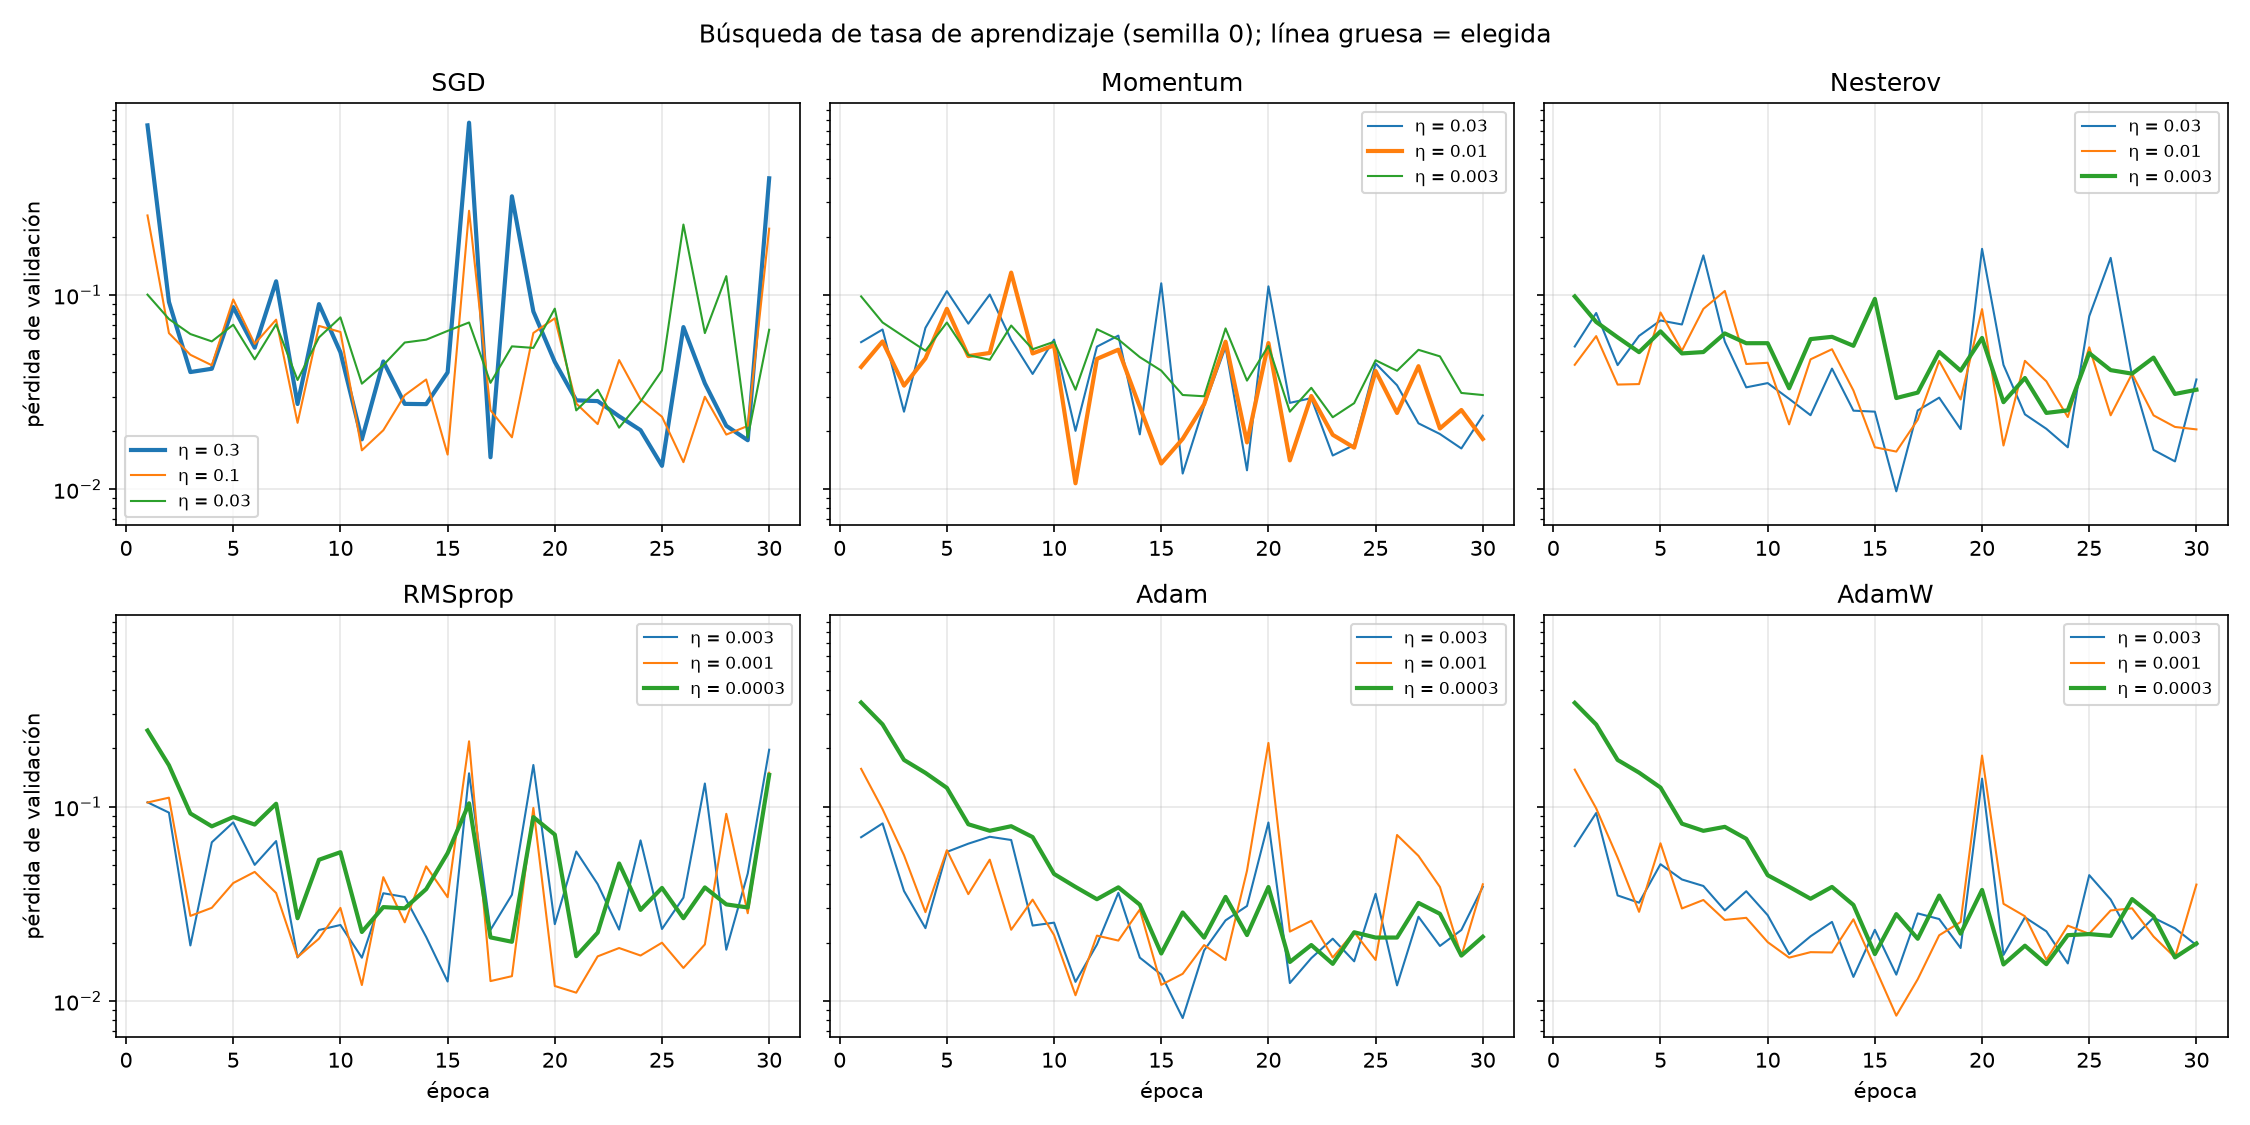
\includegraphics[width=\textwidth]{etapa4/busqueda_lr_curvas.png}
  \caption{Pérdida de validación (chb01) por época en la búsqueda de tasa, semilla 0. La línea gruesa es la tasa elegida.}
  \label{fig:busqueda_curvas}
\end{figure}

Las curvas de pérdida de validación (Figura~\ref{fig:busqueda_curvas}) muestran dos comportamientos. Con las tasas chicas de
los adaptativos ($3\times10^{-4}$) la pérdida baja de forma suave y lenta durante las primeras 10--15 épocas. Con las tasas
grandes, y sobre todo con SGD a $\eta = 0{,}3$, la pérdida salta de una época a otra en un orden de magnitud: hay épocas en las
que la red se desacomoda y se recupera en la siguiente. Es la señal de que el paso está cerca del límite de estabilidad del
lema de descenso (Sección~\ref{sec:gradiente}): en alguna dirección de curvatura alta, $\eta a$ se acerca o supera 2.

\section{Comparativa de optimizadores con cinco semillas}
\label{sec:res_comparativa}

\subsection{Resultado principal}

\begin{table}[ht]
\centering
\caption{Comparativa de optimizadores, cada uno con su tasa elegida por validación y 5 semillas. AUC de prueba: media $\pm$
desvío y rango. Época: mediana de la mejor época. Valor $p$: test de Mann-Whitney bilateral contra SGD.}
\label{tab:comparativa}
\begin{tabular}{lccccccc}
\toprule
Optimizador & $\eta$ & AUC val. & AUC prueba & Mín.--máx. & Época & $U$ & $p$ \\
\midrule
SGD      & 0,3              & 0,9982 & $\mathbf{0{,}9758 \pm 0{,}0063}$ & 0,966--0,981 & 26 & --- & --- \\
Momentum & 0,01             & 0,9984 & $0{,}9191 \pm 0{,}0341$ & 0,875--0,957 & 16 & 25 & 0,0079 \\
Nesterov & 0,003            & 0,9980 & $0{,}9196 \pm 0{,}0388$ & 0,854--0,957 & 24 & 25 & 0,0079 \\
RMSprop  & $3\times10^{-4}$ & 0,9982 & $0{,}9562 \pm 0{,}0224$ & 0,926--0,978 & 11 & 21 & 0,0952 \\
Adam     & $3\times10^{-4}$ & 0,9986 & $0{,}9171 \pm 0{,}0278$ & 0,871--0,939 & 16 & 25 & 0,0079 \\
AdamW    & $3\times10^{-4}$ & 0,9986 & $0{,}9225 \pm 0{,}0330$ & 0,873--0,960 & 16 & 25 & 0,0079 \\
\bottomrule
\end{tabular}
\end{table}

\begin{figure}[ht]
  \centering
  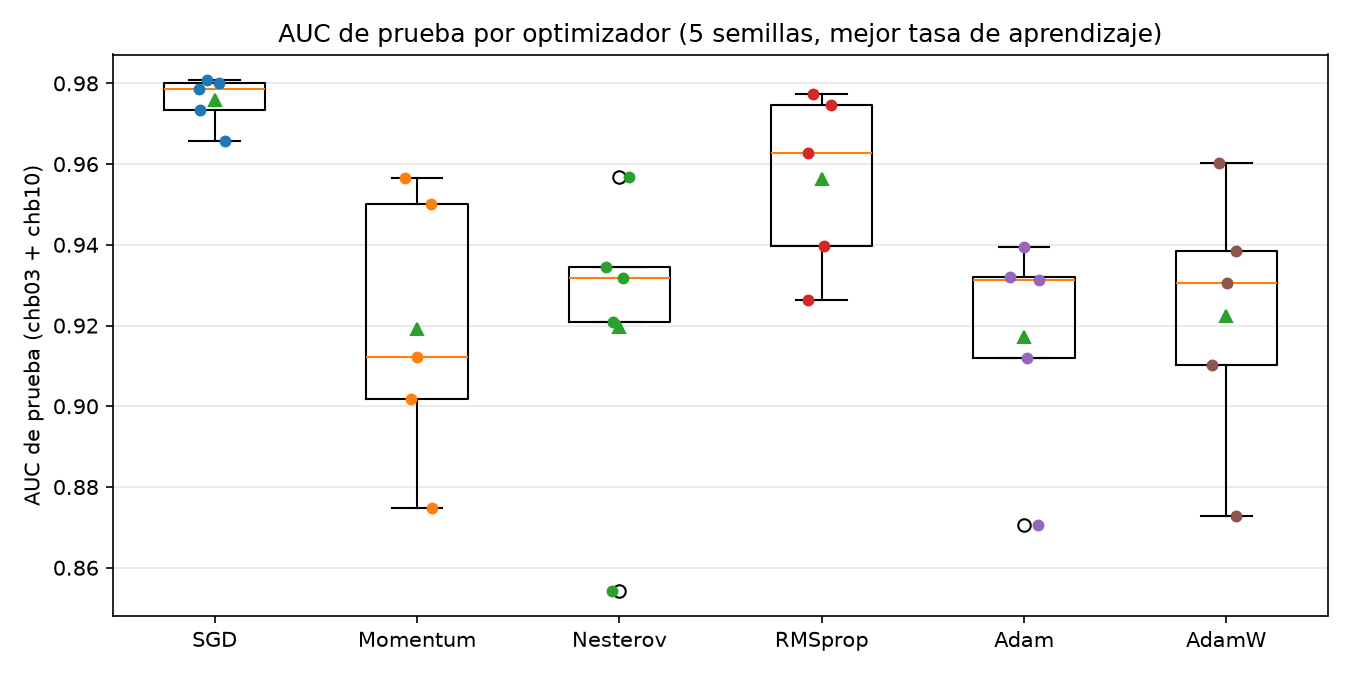
\includegraphics[width=0.9\textwidth]{etapa4/auc_prueba_por_optimizador.png}
  \caption{AUC de prueba de las 5 semillas de cada optimizador con su tasa elegida. Caja: cuartiles; línea naranja:
           mediana; triángulo: media.}
  \label{fig:auc_por_optimizador}
\end{figure}

Según la Tabla~\ref{tab:comparativa} y la Figura~\ref{fig:auc_por_optimizador}:
\begin{itemize}
  \item \textbf{SGD con $\eta = 0{,}3$ es el mejor y el más estable}: $0{,}976 \pm 0{,}006$. Su peor semilla (0,966) supera a
        la mejor de Adam (0,939).
  \item Contra Momentum, Nesterov, Adam y AdamW, las 5 semillas de SGD superan a las 5 del otro optimizador: $U = 25$,
        el máximo posible, con $p = 0{,}0079$. Es menor que el umbral de Bonferroni para 5 comparaciones ($0{,}01$), así que
        la diferencia se mantiene después de corregir.
  \item Contra RMSprop la diferencia no es significativa ($U = 21$, $p = 0{,}095$): RMSprop es el segundo, con mayor
        dispersión.
  \item Los otros cuatro quedan entre 0,917 y 0,923 de media, con desvíos de 0,03 a 0,04: la semilla mueve el resultado
        tanto como el optimizador.
  \item \textbf{El AUC de validación es prácticamente el mismo para los seis} (0,9980 a 0,9986), y ni siquiera ordena bien:
        Adam y AdamW tienen el mayor AUC de validación y están entre los peores en prueba.
\end{itemize}

Tomada al pie de la letra, la tabla coincidiría con \textcite{wilson2017}: el SGD simple generaliza mejor que los métodos
adaptativos. Pero la comparación es entre \emph{pares (optimizador, tasa)}, y la tasa la eligió un criterio que no
discrimina. Las secciones siguientes muestran que esa lectura no se sostiene.

\subsection{Curvas de entrenamiento}

\begin{figure}[ht]
  \centering
  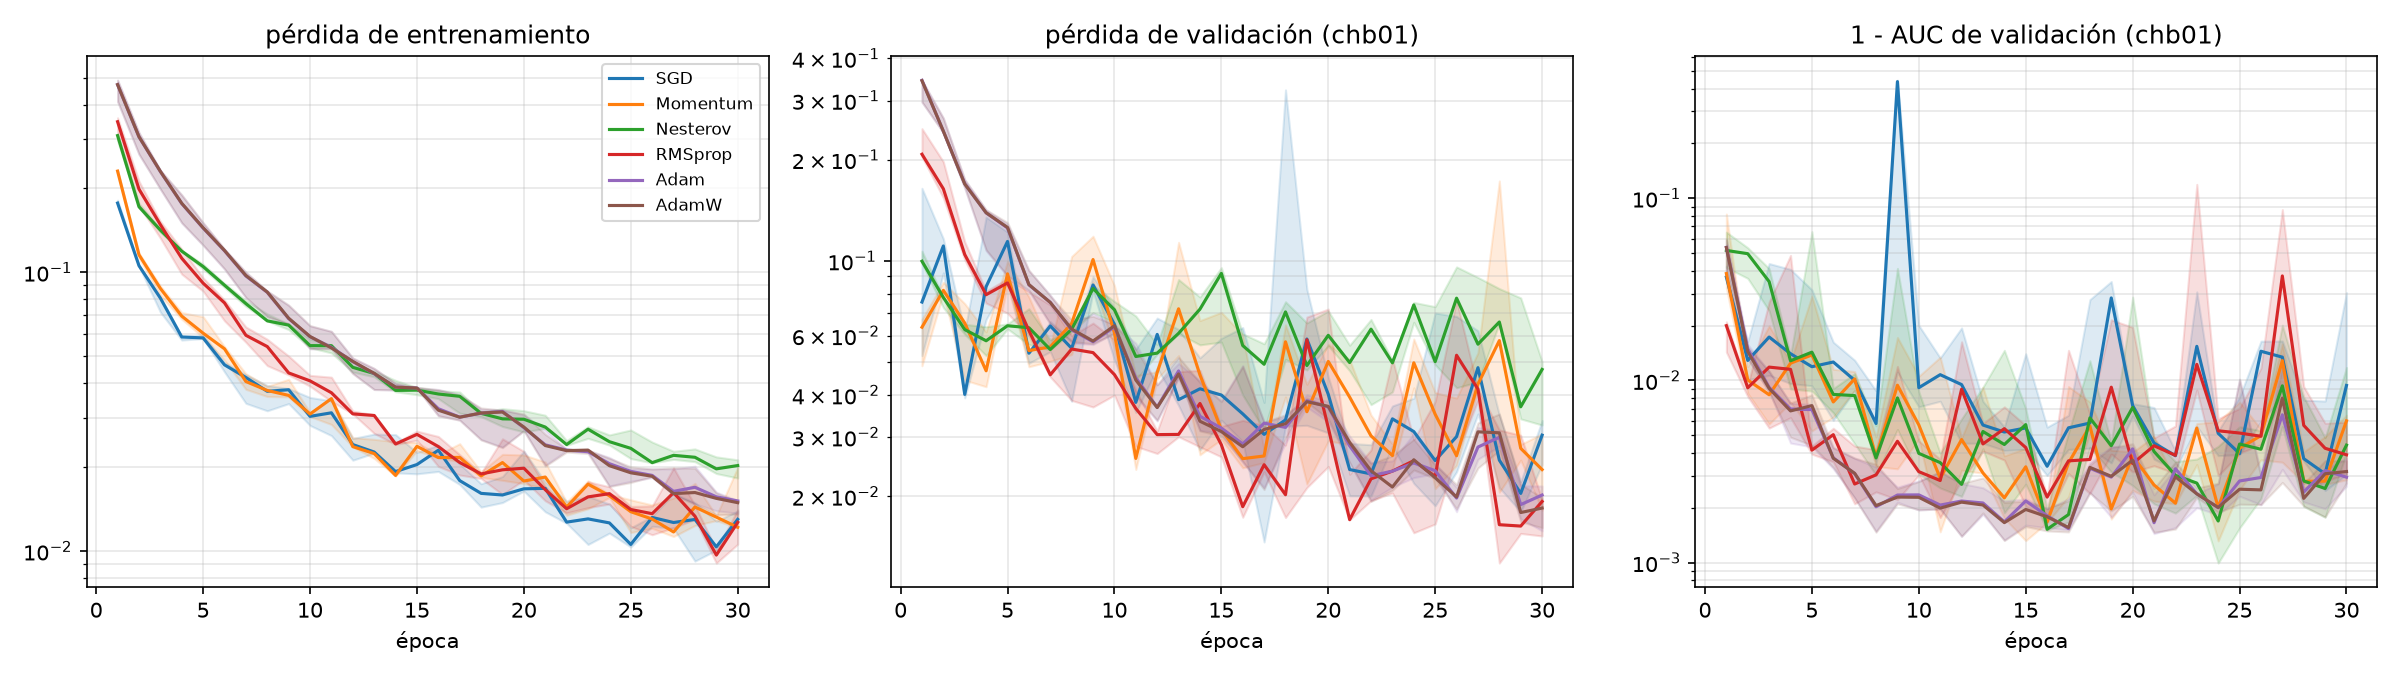
\includegraphics[width=\textwidth]{etapa4/curvas_optimizadores.png}
  \caption{Curvas de entrenamiento con la tasa elegida: mediana (línea) y rango intercuartil (sombra) sobre las 5 semillas.
           El AUC de validación se muestra como $1 - \text{AUC}$ en escala logarítmica.}
  \label{fig:curvas_optimizadores}
\end{figure}

La Figura~\ref{fig:curvas_optimizadores} muestra la evolución de las 30 épocas:
\begin{itemize}
  \item \textbf{Pérdida de entrenamiento.} SGD y Momentum bajan más rápido y terminan más abajo; Nesterov, Adam y AdamW
        quedan más arriba durante todo el entrenamiento. No es una propiedad de los algoritmos: son justamente los tres a los
        que la búsqueda les asignó la tasa más chica de su grilla. Con paso chico, en 2100 pasos la red no llega a ajustar
        tanto.
  \item \textbf{Inestabilidad de SGD.} Con $\eta = 0{,}3$, las 5 semillas tienen épocas en las que el AUC de validación cae
        de golpe por debajo de 0,7 (el mínimo es 0,21) y se recupera en la época siguiente; en la mediana se ve como el pico
        de la época 9. Momentum, con el mismo paso efectivo (0,3) en el experimento de la Sección~\ref{sec:res_tasa_alta}, no
        cae nunca por debajo de 0,81. Es lo que predice la Proposición~\ref{prop:momentum}: a igual paso efectivo, el momento
        amplía la región de estabilidad de $\eta_\text{ef}\,a < 2$ a $\eta_\text{ef}\,a < 38$. Guardar la mejor época evita
        que esas caídas afecten el resultado final.
  \item \textbf{Validación saturada.} Desde la época 8, todos los optimizadores quedan con $1 - \text{AUC}$ entre
        $2\times10^{-3}$ y $10^{-2}$ en validación (mediana de las semillas), con oscilaciones de época a época mayores que las diferencias entre optimizadores. La pérdida de
        validación, en cambio, sigue bajando lentamente: la red mejora la confianza de sus predicciones en chb01, pero el
        orden de los puntajes ya no cambia.
  \item \textbf{Mejor época.} RMSprop alcanza su mejor época antes (mediana 11) y SGD, más tarde (26). Con validación
        saturada, cuál época queda como ``mejor'' es en buena parte azar.
\end{itemize}

\section{La validación con un solo paciente no discrimina}
\label{sec:res_validacion}

\begin{figure}[ht]
  \centering
  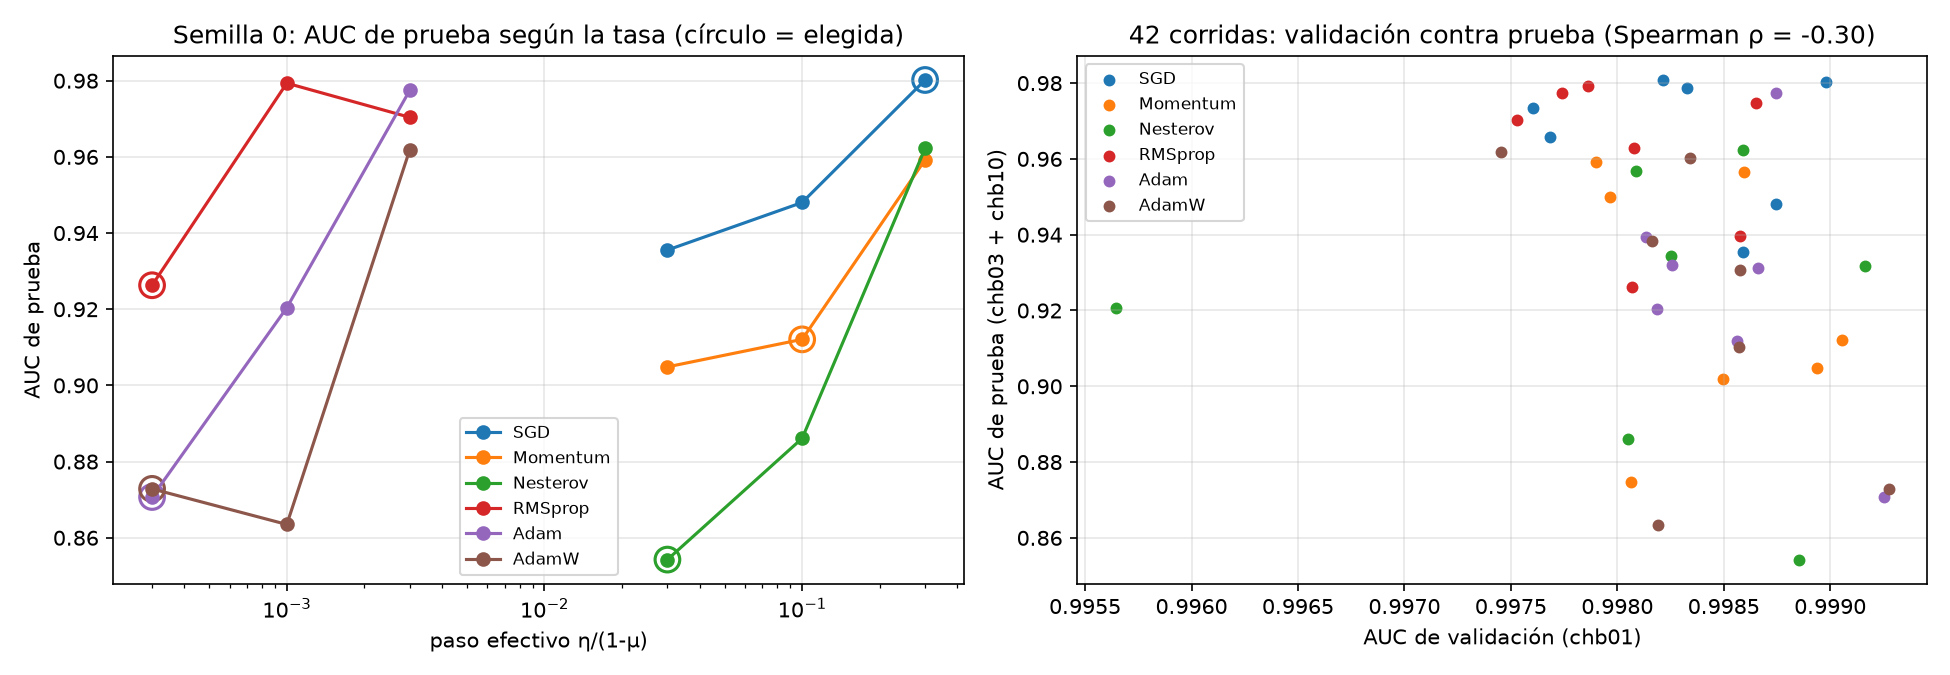
\includegraphics[width=\textwidth]{etapa4/validacion_vs_prueba.png}
  \caption{Izquierda: AUC de prueba de la semilla 0 en función del paso efectivo; el círculo marca la tasa elegida por
           validación. Derecha: AUC de validación contra AUC de prueba en las 42 corridas del diseño original.}
  \label{fig:validacion_vs_prueba}
\end{figure}

La Figura~\ref{fig:validacion_vs_prueba} resume el problema.
\begin{itemize}
  \item \textbf{Rangos.} En las 42 corridas, el AUC de validación (sobre las 36\,496 ventanas de chb01) varía entre 0,9956 y
        0,9993, y el de prueba, entre 0,854 y 0,981. La validación cambia en milésimas y la prueba, en décimas.
  \item \textbf{Correlación.} La correlación de Spearman entre ambos es $\rho = -0{,}30$ ($p = 0{,}06$). No solo no hay
        asociación positiva: la tendencia, no significativa, es la contraria. Las corridas con mayor AUC de validación
        (por encima de 0,999) incluyen algunas de las peores en prueba.
  \item \textbf{La tasa elegida.} En la semilla 0, la tasa \emph{más alta} de la grilla dio el mejor AUC de prueba en cinco
        de los seis optimizadores (en RMSprop, la del medio). La validación eligió esa tasa solo para SGD. Para Nesterov,
        Adam y AdamW eligió la que en prueba resultó peor o casi peor.
\end{itemize}

¿Por qué pasa esto? chb01 es un paciente ``fácil'': todas las redes, desde la época 8, separan sus crisis casi
perfectamente. Un conjunto de validación en el que todos los modelos aciertan no puede ordenarlos. Las diferencias entre
corridas aparecen en otro lado: en lo que la red hace con un paciente cuyas crisis son distintas de las que vio. La
Sección~\ref{sec:res_percentil} muestra exactamente dónde.

Desde el punto de vista del diseño, la lección es clara: \textbf{un solo paciente de validación no alcanza para elegir
hiperparámetros} en un problema donde lo que se busca es generalizar entre pacientes. Habría hecho falta validación
cruzada por paciente también para la búsqueda de tasa, como el LOPO del Capítulo~\ref{cap:convexos}, aunque eso
multiplica el costo de entrenamiento.

\section{Análisis por crisis}
\label{sec:res_percentil}

Para entender de dónde salen las diferencias en el AUC de prueba se calcula, para cada corrida y cada una de las 14 crisis
de prueba, el \textbf{percentil} del puntaje mediano de las ventanas de la crisis dentro de la distribución de las 78\,998
ventanas sin crisis de prueba. Un percentil de 1 significa que la crisis está por encima de todas las ventanas normales; uno
de 0,5, que no se distingue de ellas; uno cercano a 0, que la red la puntúa \emph{más bajo} que casi cualquier ventana normal.
Como el AUC es el promedio, sobre las ventanas ictales, de la fracción de negativos que cada una supera
(Proposición~\ref{prop:auc}), este percentil es su versión por crisis.

\begin{figure}[ht]
  \centering
  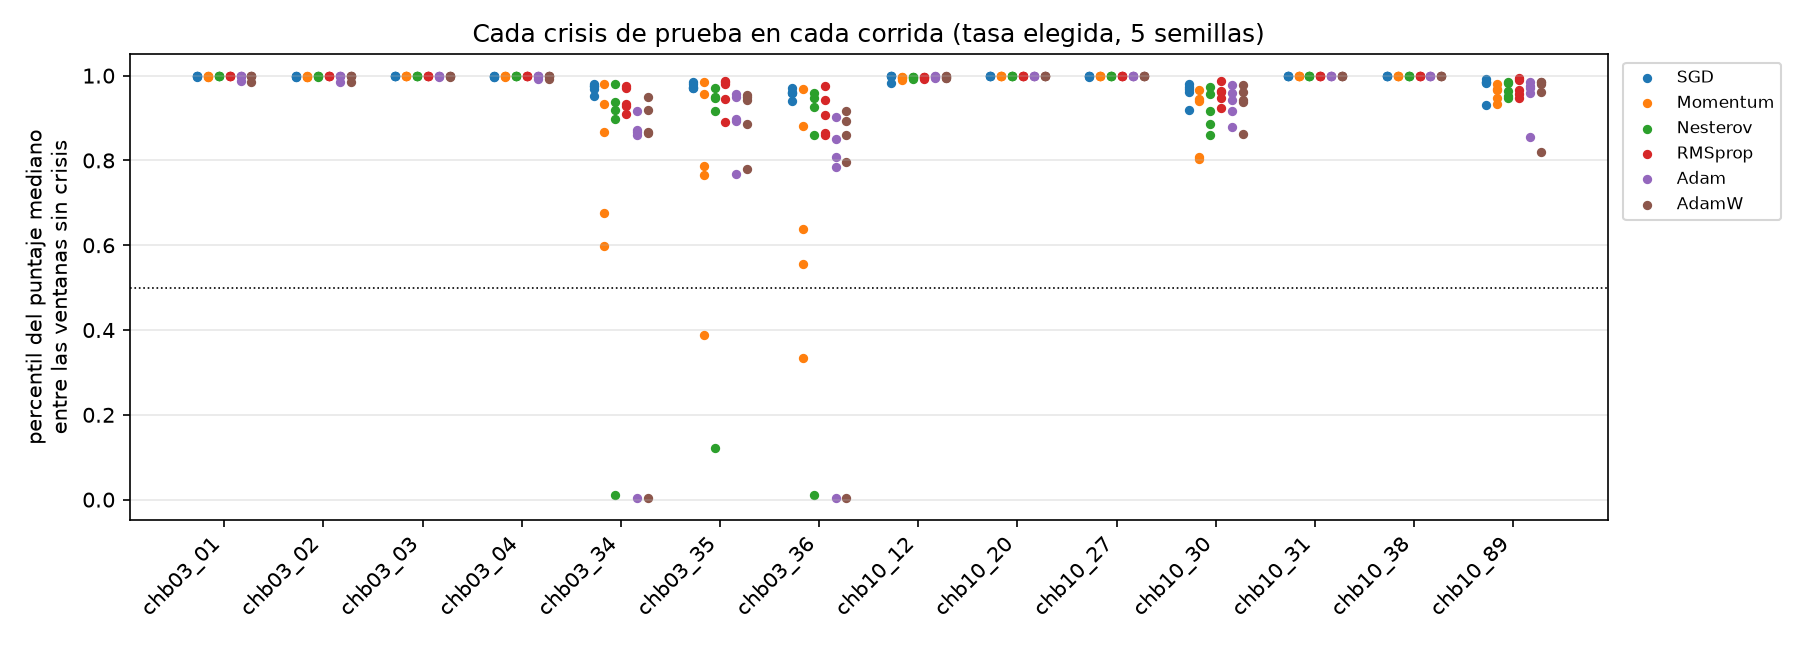
\includegraphics[width=\textwidth]{etapa4/percentil_por_crisis.png}
  \caption{Percentil del puntaje mediano de cada crisis de prueba entre las ventanas sin crisis, para las 30 corridas con la
           tasa elegida (5 semillas por optimizador). La línea punteada es 0,5 (indistinguible del azar).}
  \label{fig:percentil_crisis}
\end{figure}

\begin{table}[ht]
\centering
\caption{Percentil medio de las tres crisis difíciles de chb03 por optimizador (tasa elegida, 5 semillas). Las otras 11
crisis tienen percentil medio de 0,93 o más.}
\label{tab:percentil_opt}
\begin{tabular}{lccc}
\toprule
Optimizador & chb03\_34 & chb03\_35 & chb03\_36 \\
\midrule
SGD      & 0,971 & 0,976 & 0,958 \\
RMSprop  & 0,944 & 0,958 & 0,910 \\
Momentum & 0,811 & 0,777 & 0,676 \\
Nesterov & 0,749 & 0,782 & 0,741 \\
Adam     & 0,704 & 0,893 & 0,670 \\
AdamW    & 0,721 & 0,902 & 0,694 \\
\bottomrule
\end{tabular}
\end{table}

Los resultados (Figura~\ref{fig:percentil_crisis} y Tabla~\ref{tab:percentil_opt}) son muy concentrados:
\begin{itemize}
  \item \textbf{11 de las 14 crisis las reconocen bien todas las corridas.} Las cuatro primeras de chb03 y las siete de chb10
        tienen percentil medio entre 0,93 y 1, con desvío entre corridas menor a 0,05.
  \item \textbf{Toda la variabilidad está en tres crisis de un mismo paciente}: chb03\_34, chb03\_35 y chb03\_36, de los
        registros del final de la internación. Su desvío entre corridas es de 0,2 a 0,3. En algunas corridas, entre ellas el
        modelo final (AdamW, semilla 0) y Adam con semilla 0, dos de ellas quedan con percentil 0,004: \emph{por debajo del 99,6~\% de las ventanas
        normales}.
  \item El percentil medio de esas tres crisis explica el ranking de prueba: su correlación de Spearman con el AUC de prueba,
        sobre las 42 corridas, es $\rho = 0{,}87$ ($p < 10^{-13}$).
  \item La Tabla~\ref{tab:percentil_opt} reproduce la separación de la Tabla~\ref{tab:comparativa}: SGD y RMSprop
        puntúan alto esas tres crisis en todas sus semillas; los otros cuatro, con la tasa elegida, no siempre.
\end{itemize}

La consecuencia para la comparativa es importante: \textbf{el conjunto de prueba efectivo para distinguir optimizadores son
tres crisis de un paciente}. Todas las conclusiones sobre qué optimizador es mejor dependen de qué pasa con ellas, y no se
pueden generalizar mucho más allá de este caso.

\section{Experimento de sensibilidad: todos con la tasa alta}
\label{sec:res_tasa_alta}

La búsqueda sugería que la ventaja de SGD podía deberse a la tasa y no al algoritmo: a SGD la validación le dio la tasa
alta, y a los demás no. Para probarlo, se corrió cada optimizador con la tasa más alta de su grilla y 5 semillas. Este
experimento se diseñó \textbf{después de mirar la prueba}, así que es exploratorio: no cambia el modelo elegido ni las
conclusiones de las Secciones~\ref{sec:res_comparativa} y~\ref{sec:res_clinica}, y sus valores $p$ no tienen la
interpretación de un test planificado.

\begin{table}[ht]
\centering
\caption{Experimento exploratorio: cada optimizador con la tasa más alta de su grilla, 5 semillas. Se repite la media con la
tasa elegida para comparar. Valor $p$: Mann-Whitney bilateral contra SGD.}
\label{tab:tasa_alta}
\begin{tabular}{lcccccc}
\toprule
 & & \multicolumn{3}{c}{Tasa alta} & Tasa elegida & \\
\cmidrule(lr){3-5}\cmidrule(lr){6-6}
Optimizador & $\eta$ & AUC val. & AUC prueba & Mín. & AUC prueba & $p$ \\
\midrule
SGD      & 0,3              & 0,9982 & $0{,}9758 \pm 0{,}0063$ & 0,966 & 0,9758 & --- \\
Momentum & 0,03             & 0,9979 & $0{,}9596 \pm 0{,}0067$ & 0,950 & 0,9191 & 0,016 \\
Nesterov & 0,03             & 0,9987 & $0{,}9501 \pm 0{,}0285$ & 0,905 & 0,9196 & 0,056 \\
RMSprop  & $3\times10^{-3}$ & 0,9976 & $0{,}9730 \pm 0{,}0132$ & 0,952 & 0,9562 & 1,000 \\
Adam     & $3\times10^{-3}$ & 0,9984 & $0{,}9712 \pm 0{,}0091$ & 0,957 & 0,9171 & 0,310 \\
AdamW    & $3\times10^{-3}$ & 0,9975 & $0{,}9699 \pm 0{,}0076$ & 0,962 & 0,9225 & 0,222 \\
\bottomrule
\end{tabular}
\end{table}

\begin{figure}[ht]
  \centering
  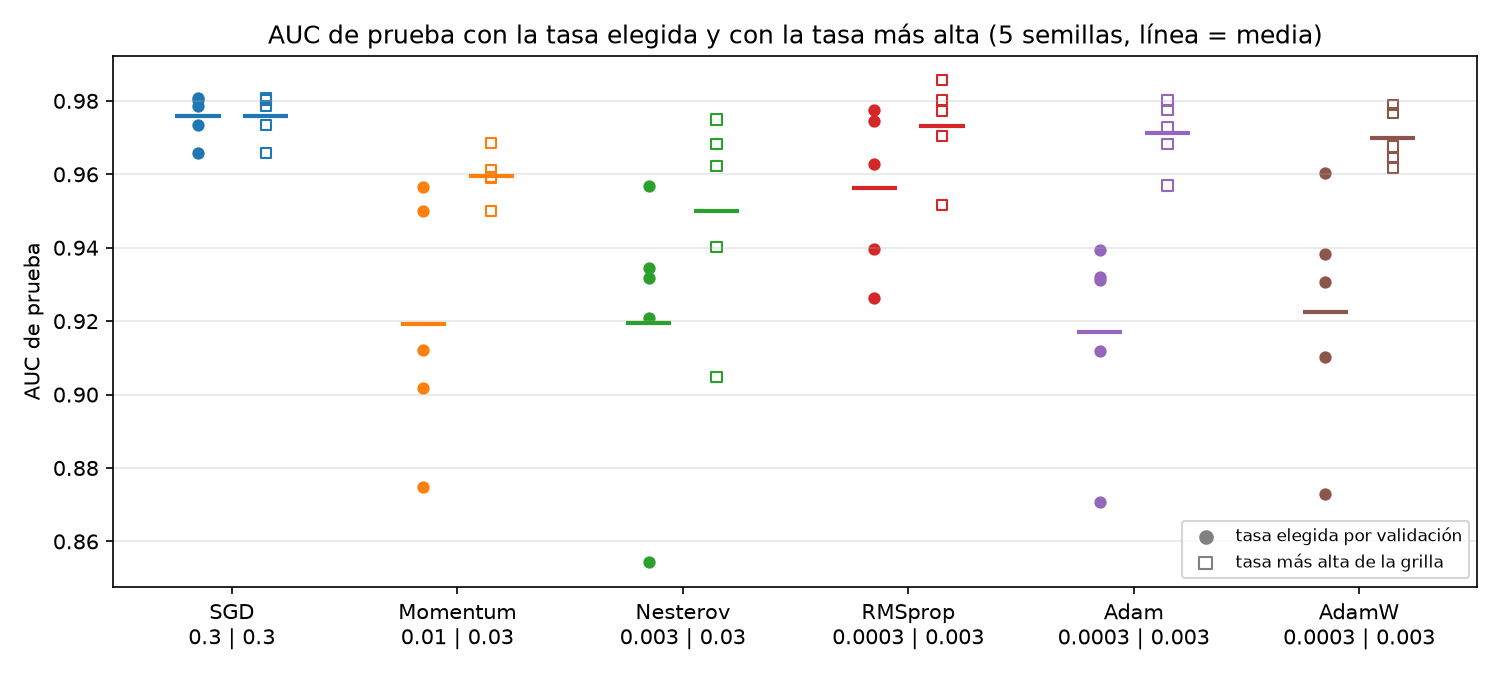
\includegraphics[width=\textwidth]{etapa4/tasa_elegida_vs_alta.png}
  \caption{AUC de prueba de las 5 semillas de cada optimizador con la tasa elegida por validación (círculos) y con la tasa
           más alta de la grilla (cuadrados). La línea horizontal es la media.}
  \label{fig:tasa_alta}
\end{figure}

La Tabla~\ref{tab:tasa_alta} y la Figura~\ref{fig:tasa_alta} confirman la hipótesis:
\begin{itemize}
  \item \textbf{Con la tasa alta, todos mejoran} y la dispersión baja mucho. Adam pasa de $0{,}917 \pm 0{,}028$ a
        $0{,}971 \pm 0{,}009$; AdamW, de $0{,}923 \pm 0{,}033$ a $0{,}970 \pm 0{,}008$.
  \item \textbf{RMSprop, Adam y AdamW quedan empatados con SGD}: medias entre 0,970 y 0,976, y valores $p$ entre 0,22 y 1.
        La ``ventaja de SGD sobre los adaptativos'' de la Tabla~\ref{tab:comparativa} era, sobre todo, una ventaja de la tasa.
  \item \textbf{Momentum} queda algo por debajo (0,960) con el mismo paso efectivo que SGD. La diferencia es consistente
        (SGD gana en 24 de los 25 pares de semillas, $U = 24$, $p = 0{,}016$) pero no pasa la corrección de Bonferroni.
  \item \textbf{Nesterov} sigue siendo el más irregular: una semilla en 0,905 y desvío de 0,029.
  \item \textbf{La validación tampoco habría elegido estas tasas}: su AUC de validación medio (0,9975 a 0,9987) es igual o
        menor que el de las tasas elegidas. El problema no es la regla de elección sino que chb01 no discrimina.
\end{itemize}

\subsection{Interpretación}

¿Por qué la tasa alta generaliza mejor a chb03? No hay una demostración, pero hay tres elementos consistentes con lo
observado:
\begin{enumerate}
  \item \textbf{Ruido y mínimos planos.} Con paso grande, el ruido del gradiente estocástico impide que la red se acomode en
        regiones angostas de la pérdida, que tienden a depender de detalles de los tres pacientes de entrenamiento.
        Las caídas de validación de SGD con $\eta = 0{,}3$ muestran que el entrenamiento está, efectivamente, cerca del borde
        de la estabilidad.
  \item \textbf{Normalización por lotes.} Por la Proposición~\ref{prop:bn_escala}, la tasa efectiva de las capas convolucionales
        depende de $\eta/\lVert\vw\rVert^2$. Con tasa alta las normas crecen más rápido, y la dinámica cambia en formas que no se
        reducen a ``más paso''.
  \item \textbf{Menos ajuste a los pacientes de entrenamiento.} Con tasa chica, Adam y AdamW tienen la pérdida de
        entrenamiento más alta (Figura~\ref{fig:curvas_optimizadores}), pero aun así generalizan peor. No es un problema de
        sobreajuste clásico (más pérdida de entrenamiento con peor prueba), sino de \emph{qué} solución se encuentra entre
        muchas con pérdida parecida, que es lo esperable en una función no convexa (Sección~\ref{sec:no_convexo}).
\end{enumerate}

La conclusión de la comparativa, con la cautela que impone haber diseñado este experimento después de ver la prueba, es que
\textbf{en este problema el factor que más pesa en la generalización a pacientes nuevos es la tasa de aprendizaje, más que el
algoritmo}. Con la tasa adecuada, los seis optimizadores quedan entre 0,95 y 0,98, y SGD, RMSprop, Adam y AdamW no se
distinguen con 5 semillas.

\section{Evaluación clínica del modelo elegido}
\label{sec:res_clinica}

\subsection{El modelo elegido}

El protocolo elige el optimizador con mayor AUC de validación medio y, dentro de él, la semilla con mayor AUC de validación.
Resulta \textbf{AdamW con $\eta = 3\times10^{-4}$, semilla 0} (AUC de validación 0,9993, mejor época 15). Adam y AdamW
empatan en 0,9986 de AUC de validación medio, y el desempate a la cuarta cifra favorece a AdamW.

Con lo visto en las secciones anteriores, es una mala elección: en prueba es una de las peores corridas (AUC 0,873). Se
informa igual. Cambiar el modelo después de mirar la prueba invalidaría la estimación de su desempeño, que es lo que el
conjunto de prueba debe dar. Es preferible informar un modelo peor con una estimación honesta que uno mejor con una
estimación sesgada.

\subsection{Métricas por ventana y por evento}

Se aplica el procedimiento de la Sección~\ref{sec:umbral_np}: suavizado causal de 3 ventanas y umbral de Neyman-Pearson con
$\alpha = 10^{-3}$ calculado con las ventanas sin crisis de chb01.

\begin{figure}[ht]
  \centering
  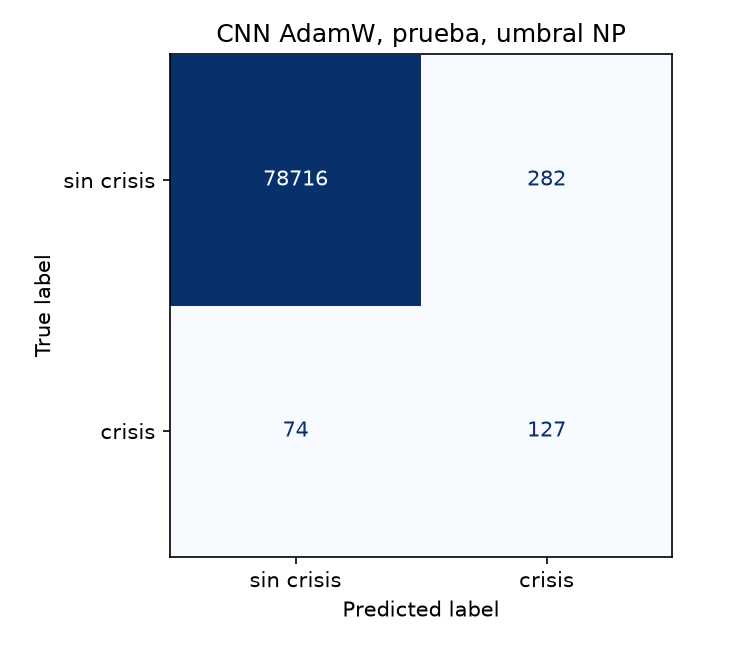
\includegraphics[width=0.5\textwidth]{etapa4/confusion_cnn.png}
  \caption{Matriz de confusión por ventana de la CNN final en prueba (chb03 y chb10, sin ventanas de borde), con umbral de
           Neyman-Pearson.}
  \label{fig:confusion_cnn}
\end{figure}

\begin{table}[ht]
\centering
\caption{CNN final (AdamW, semilla 0) en los pacientes de prueba, umbral de Neyman-Pearson con $\alpha = 10^{-3}$.}
\label{tab:cnn_pacientes}
\begin{tabular}{lccc}
\toprule
 & chb03 & chb10 & Total \\
\midrule
AUC                         & 0,726 & 0,995 & 0,872 \\
$TP$ / $FN$                 & 46 / 50 & 81 / 24 & 127 / 74 \\
$FP$ / $TN$                 & 242 / 33\,853 & 40 / 44\,863 & 282 / 78\,716 \\
Sensibilidad por ventana    & 0,479 & 0,771 & 0,632 \\
Especificidad por ventana   & 0,9929 & 0,9991 & 0,9964 \\
VPP por ventana             & 0,160 & 0,669 & 0,311 \\
Crisis detectadas           & 4/7 & 7/7 & 11/14 \\
Horas sin crisis            & 37,9 & 49,9 & 87,8 \\
Falsas alarmas              & 98 & 21 & 119 \\
Falsas alarmas por hora     & 2,59 & 0,42 & 1,36 \\
Latencia mediana [s]        & 9 & 11 & 11 \\
\bottomrule
\end{tabular}
\end{table}

La Tabla~\ref{tab:cnn_pacientes} y la Figura~\ref{fig:confusion_cnn} muestran dos pacientes muy distintos.
\begin{itemize}
  \item \textbf{chb10 sale casi perfecto}: AUC 0,995, las 7 crisis detectadas con una latencia mediana de 11~s y 0,42 falsas
        alarmas por hora (una cada dos horas y media).
  \item \textbf{chb03 es el paciente difícil}: AUC 0,73. Se detectan las 4 crisis de los registros chb03\_01 a chb03\_04, con
        latencias de 6 a 13~s, pero ninguna de las de chb03\_34 a chb03\_36. Además genera 2,6 falsas alarmas por hora.
\end{itemize}

Las crisis no detectadas no son ``débiles'': respecto del resto de su registro, tienen un aumento de potencia por banda
\emph{mayor} que las detectadas (del orden de 1,7 contra 1,2 en $\log_{10}$), y la regresión logística calibrada, que solo
mira la potencia por banda, les da puntajes altos. La red aprendió de los tres pacientes de entrenamiento un patrón
espectro-temporal más específico que ``sube la potencia'', y ese patrón no aparece en estas tres crisis. Es el precio de un
modelo más expresivo entrenado con 13 crisis.

\paragraph{La restricción de Neyman-Pearson en cada paciente.} Con $\alpha = 10^{-3}$ y 900 ventanas por hora se esperan
unas 0,9 ventanas falsas por hora. En chb10 hay $40/49{,}9 = 0{,}8$: la restricción se cumple. En chb03 hay
$242/37{,}9 = 6{,}4$, siete veces más. Es otra vez la Observación~\ref{obs:np_supuesto}: el umbral se calibró con la
distribución del puntaje de chb01, y la de chb03 tiene la cola derecha más pesada. Una calibración del umbral con un
período inicial del propio paciente lo corregiría en buena parte.

\paragraph{Valor predictivo.} De las 409 ventanas declaradas como crisis, 127 lo son: VPP de 0,31, como se anticipó con la
ecuación~\eqref{eq:vpp_bayes}. Por evento, las 282 ventanas falsas se agrupan en 119 alarmas.

\section{Comparación con los modelos convexos}
\label{sec:res_comparacion}

\begin{table}[ht]
\centering
\caption{Partición fija, prueba en chb03 y chb10 (14 crisis, 87,8 horas sin crisis). Suavizado de 3 ventanas y umbral de
Neyman-Pearson con $\alpha = 10^{-3}$ calibrado en chb01. ``Sens. a $10^{-3}$'': sensibilidad por ventana con una tasa de
falsos positivos de $10^{-3}$ en la propia prueba (leída de la curva ROC).}
\label{tab:comparacion_final}
\begin{tabular}{lccccccc}
\toprule
Modelo & AUC & Sens. a $10^{-3}$ & Sens. & Espec. & Crisis & FA/h & Lat. [s] \\
\midrule
Logística (global)     & 0,799 & 0,00 & 0,304 & 0,9849 & 5/14 & 3,26 & 14,0 \\
SVM lineal (global)    & 0,798 & 0,00 & 0,304 & 0,9865 & 7/14 & 2,94 & 18,0 \\
Logística (calibrada)  & \textbf{0,934} & 0,02 & 0,269 & 0,9941 & 7/14 & 1,22 & 26,0 \\
SVM lineal (calibrado) & 0,930 & 0,02 & 0,244 & 0,9946 & 6/14 & \textbf{1,00} & 24,5 \\
CNN AdamW              & 0,872 & \textbf{0,54} & \textbf{0,632} & \textbf{0,9964} & \textbf{11/14} & 1,36 & \textbf{11,0} \\
\bottomrule
\end{tabular}
\end{table}

\begin{figure}[ht]
  \centering
  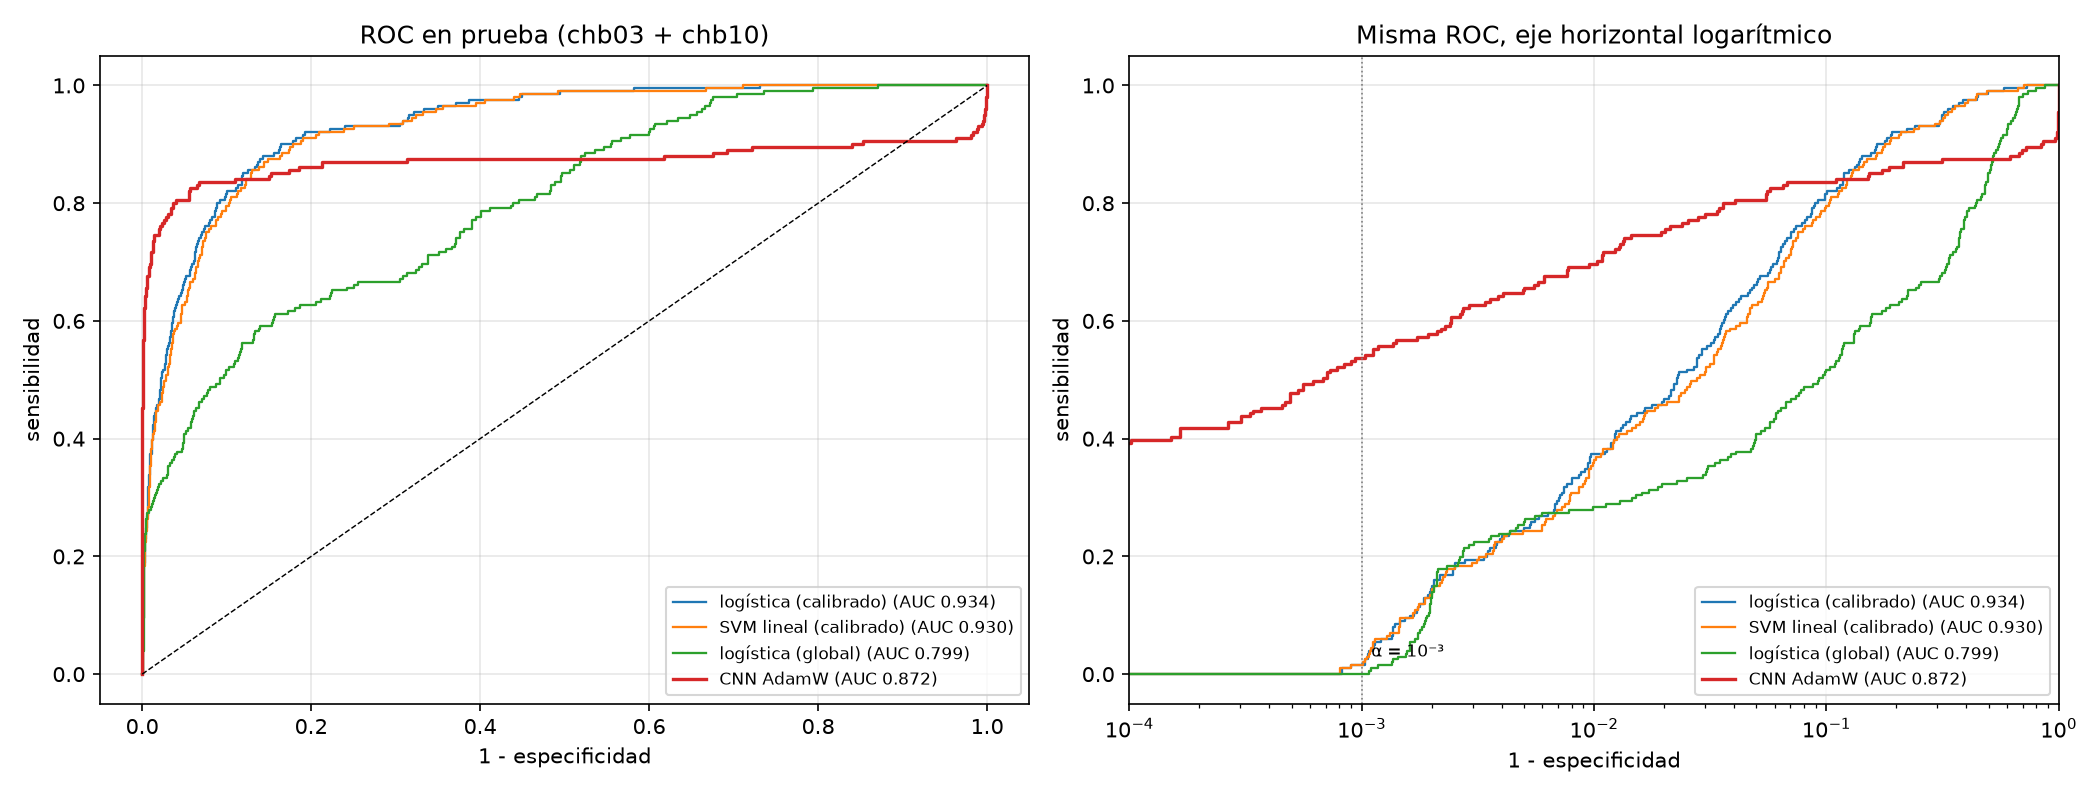
\includegraphics[width=\textwidth]{etapa4/roc_cnn_vs_convexos.png}
  \caption{Curvas ROC en prueba de la CNN final y de los modelos convexos. Izquierda: ejes lineales. Derecha: eje horizontal
           logarítmico; la línea punteada marca $\text{FPR} = 10^{-3}$.}
  \label{fig:roc_cnn}
\end{figure}

La Tabla~\ref{tab:comparacion_final} y la Figura~\ref{fig:roc_cnn} muestran el caso que se anticipó en la
Sección~\ref{sec:zona_util}: \textbf{el modelo con menor AUC es el mejor detector}.
\begin{itemize}
  \item En ejes lineales, la logística calibrada parece mejor: su curva está por encima de la de la CNN desde un 12~\% de
        falsos positivos, y su AUC es 0,934 contra 0,872.
  \item En escala logarítmica la situación se invierte. Con $\text{FPR} = 10^{-3}$ (0,9 ventanas falsas por hora), la CNN detecta
        el 54~\% de las ventanas ictales y la logística calibrada, el 2~\%: su curva recién despega a partir de $10^{-3}$. Con
        $\text{FPR} = 10^{-4}$ la CNN todavía detecta el 39~\% y la logística, ninguna. Con $\text{FPR} = 10^{-2}$: 70~\% contra 37~\%.
  \item La curva de la CNN casi \textbf{se estanca} desde un 10~\% de falsos positivos: pasa de 0,84 a solo 0,90 con 95~\% de
        falsos positivos, mientras la logística llega a 0,99 con 50~\%. Las ventanas de chb03\_34 a chb03\_36 tienen un puntaje
        menor que la mayoría de las ventanas normales. Ese tramo es el que hunde el AUC, en una zona de la curva (más de
        10~\% de falsos positivos, 90 ventanas falsas por hora) que no tiene ningún uso clínico.
\end{itemize}

En términos de la Sección~\ref{sec:neyman_pearson}: el punto de operación está donde la pendiente de la ROC es igual al
multiplicador $\lambda$, que con $\alpha$ chico es grande. La CNN tiene una curva muy empinada al principio (muchas crisis con
puntajes que ninguna ventana normal alcanza) y la logística no. El AUC promedia toda la curva con el mismo peso y no ve esa
diferencia. Para detección de crisis conviene informar la sensibilidad con una tasa fija de falsos positivos, o el AUC parcial
hasta $\text{FPR} = 10^{-2}$.

Por evento, la CNN detecta 11 crisis contra 7 de la logística calibrada, con una cantidad de falsas alarmas parecida
(1,36 contra 1,22 por hora) y menos de la mitad de latencia (11~s contra 26~s).

\section{El compromiso clínico: barrido de $\alpha$}
\label{sec:res_barrido}

El nivel $\alpha = 10^{-3}$ es una elección. Variándolo se obtiene la curva completa de sensibilidad por evento contra falsas
alarmas por hora, la versión clínica de la curva ROC. Para cada $\alpha$ el umbral se recalcula en chb01 y se aplica a la
prueba.

\begin{table}[ht]
\centering
\caption{Barrido del nivel $\alpha$ del umbral de Neyman-Pearson en los pacientes de prueba (14 crisis, 87,8 horas sin crisis).
Sens.: sensibilidad por evento.}
\label{tab:barrido_alfa}
\begin{tabular}{ccccccc}
\toprule
 & \multicolumn{3}{c}{CNN AdamW} & \multicolumn{3}{c}{Logística calibrada} \\
\cmidrule(lr){2-4}\cmidrule(lr){5-7}
$\alpha$ & Sens. & FA/h & Lat. [s] & Sens. & FA/h & Lat. [s] \\
\midrule
$3\times10^{-5}$ & 0,500 (7) & 0,00 & 24,0 & 0,286 (4) & 0,29 & 41,0 \\
$10^{-4}$        & 0,571 (8) & 0,00 & 31,0 & 0,357 (5) & 0,43 & 34,0 \\
$3\times10^{-4}$ & 0,714 (10) & 0,19 & 19,5 & 0,429 (6) & 0,54 & 35,0 \\
$10^{-3}$        & 0,786 (11) & 1,36 & 11,0 & 0,500 (7) & 1,22 & 26,0 \\
$3\times10^{-3}$ & 0,929 (13) & 3,71 & 10,0 & 0,714 (10) & 3,94 & 17,5 \\
$10^{-2}$        & 0,929 (13) & 8,41 & 6,0  & 1,000 (14) & 11,63 & 15,5 \\
$3\times10^{-2}$ & 1,000 (14) & 15,23 & 5,0 & 1,000 (14) & 22,17 & 10,0 \\
\bottomrule
\end{tabular}
\end{table}

\begin{figure}[ht]
  \centering
  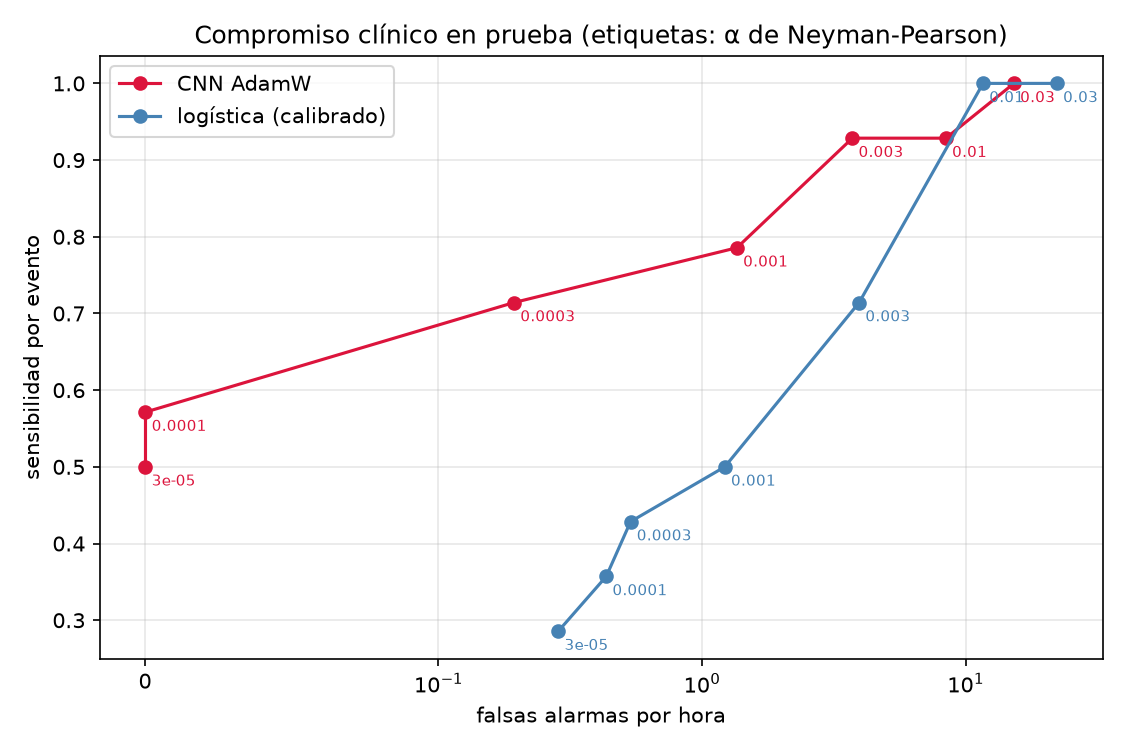
\includegraphics[width=0.8\textwidth]{etapa4/sensibilidad_vs_falsas_alarmas.png}
  \caption{Sensibilidad por evento contra falsas alarmas por hora en prueba, variando $\alpha$ (etiquetas). Eje horizontal
           lineal cerca de cero y logarítmico por encima de 0,1.}
  \label{fig:sens_fa}
\end{figure}

La Tabla~\ref{tab:barrido_alfa} y la Figura~\ref{fig:sens_fa} muestran:
\begin{itemize}
  \item \textbf{La CNN domina a la logística en toda la zona de pocas falsas alarmas.} Con $\alpha = 10^{-4}$ detecta 8 de 14
        crisis sin ninguna falsa alarma en 88 horas; con $\alpha = 3\times10^{-4}$, 10 de 14 con 0,19 falsas alarmas por hora
        (una cada 5 horas). La logística, para detectar 6 de 14, ya da 0,54 por hora.
  \item \textbf{La CNN también avisa antes}, para cualquier $\alpha$ a partir de $3\times10^{-4}$.
  \item \textbf{El compromiso es el que predice Neyman-Pearson}: al aflojar la restricción sube la sensibilidad y suben las
        falsas alarmas. El multiplicador $\lambda = dP_D/dP_{FA}$ se ve en la pendiente de la curva: entre $\alpha = 10^{-4}$ y
        $3\times10^{-4}$, la CNN gana 2 crisis por 0,19 falsas alarmas por hora; entre $10^{-2}$ y $3\times10^{-2}$, gana 1 crisis
        por 7 falsas alarmas por hora. Los rendimientos son decrecientes, como corresponde a una curva cóncava.
  \item \textbf{Detectar el 100~\% de las crisis es inaceptable con ambos modelos}: 15 falsas alarmas por hora con la CNN y 12
        con la logística.
  \item Con $\alpha \ge 10^{-2}$ la logística alcanza a la CNN en sensibilidad: las tres crisis que la CNN puntúa bajo sí las
        detecta la logística, pero solo cuando el umbral ya es muy permisivo.
\end{itemize}

Un punto de operación razonable para un monitor en una unidad de epilepsia sería $\alpha = 3\times10^{-4}$: 71~\% de las crisis
detectadas, con latencia mediana de 20~s y una falsa alarma cada 5 horas. Hay que tener presente que esos números salen de dos
pacientes y 14 crisis.

\section{Síntesis}
\label{sec:res_sintesis}

\begin{enumerate}
  \item Con la tasa elegida por validación, SGD supera significativamente a Momentum, Nesterov, Adam y AdamW
        ($p = 0{,}008$ en los cuatro casos), y no se distingue de RMSprop.
  \item Esa ventaja se explica casi por completo por la tasa de aprendizaje: en el experimento exploratorio con la tasa más
        alta de cada grilla, SGD, RMSprop, Adam y AdamW quedan empatados entre 0,970 y 0,976.
  \item La validación con un solo paciente está saturada (AUC de 0,996 a 0,999) y no predice la prueba ($\rho = -0{,}30$). Es la
        principal debilidad del diseño.
  \item Las diferencias en prueba se concentran en tres crisis de chb03; las otras 11 las reconocen todas las corridas.
  \item El modelo elegido, una de las peores corridas, detecta 11 de 14 crisis con 1,36 falsas alarmas por hora y 11~s de
        latencia, frente a 7 de 14, 1,22 y 26~s de la regresión logística calibrada, a pesar de tener menor AUC.
  \item El AUC no es la métrica adecuada para elegir un detector de crisis: lo que importa es la zona de $\text{FPR} \lesssim 10^{-3}$.
\end{enumerate}

\chapter{Discusión y conclusiones}
\label{cap:conclusiones}

\section{Discusión}

La discusión sigue el recorrido del trabajo: el fenómeno, los atributos, la optimización y la evaluación. En cada punto
se contrasta lo que predecía la teoría con lo que mostraron los datos.

\subsection{El fenómeno y los atributos de Fourier}

El modelo del Capítulo~\ref{cap:fenomeno} describe la crisis como una descarga rítmica, con fundamental $f_0$ y
armónicos (ecuación~\eqref{eq:descarga}), que se suma a la actividad de fondo y queda multiplicada por una ganancia
propia de cada paciente y canal (ecuación~\eqref{eq:modelo_eeg}). Los datos lo confirmaron en sus tres aspectos:
\begin{itemize}
  \item \textbf{Aumento de potencia concentrado en una banda.} En Bonn el set ictal tiene de 10 a 100 veces más potencia
        entre 3 y 25~Hz, con máximo cerca de 6~Hz, y la banda dominante pasa a ser theta (Tabla~\ref{tab:bonn_bandas}).
        Con solo 20 atributos de Welch, la regresión logística llega a 97,4~\% de exactitud en tres clases y el SVM con
        núcleo RBF, a 98,4~\% (Tabla~\ref{tab:bonn_cv}).
  \item \textbf{La banda cambia entre pacientes.} En CHB-MIT la banda con mayor aumento es delta en chb01 y chb08, y alfa y
        beta en chb05 y chb10 (Tabla~\ref{tab:dif_log}). No hay una ``frecuencia de la crisis'' universal. Esto motiva usar
        varias bandas como atributos y, en la red, convoluciones que se desplazan a lo largo de la frecuencia.
  \item \textbf{La ganancia de cada paciente es un término aditivo en escala logarítmica.} Restar la mediana del paciente lo
        elimina (ecuación~\eqref{eq:calibracion}). Con la partición fija, el AUC de la regresión logística pasa de 0,80 a
        0,93 y las falsas alarmas, de 3,3 a 1,2 por hora (Tabla~\ref{tab:fija_convexos}). Es la mejora más grande del
        trabajo y la produce una operación de una línea, deducida del modelo.
\end{itemize}

El modelo también tiene límites. Las tres crisis de chb03 que la red no detecta tienen un aumento de potencia por banda
\emph{mayor} que las que sí detecta. Un detector que solo mira cuánta potencia hay las encuentra; uno que aprendió la
\emph{forma} espectro-temporal de 13 crisis de otros tres pacientes, no. La ecuación~\eqref{eq:descarga} describe una
descarga estacionaria, y las crisis reales evolucionan en frecuencia y en distribución espacial a lo largo de su duración
(Figura~\ref{fig:chb01_espectrograma}).

\subsection{Optimalidad local y global}

La teoría del Capítulo~\ref{cap:optimizacion} se verificó numéricamente en los dos regímenes:
\begin{itemize}
  \item \textbf{Problema convexo.} La regresión logística regularizada es fuertemente convexa
        (Proposición~\ref{prop:logistica_convexa}). Desde 20 puntos iniciales a distancia media 13 del óptimo, el descenso por
        gradiente con paso $1/L$ llega al mismo valor $J^* = 0{,}07699786$ con distancia máxima $3\times10^{-7}$ entre
        soluciones. La convergencia es lineal, con una pendiente compatible con $\kappa \approx 528$
        (Teorema~\ref{teo:convergencia}). Todo mínimo local es global (Teorema~\ref{teo:local_global}) y una sola corrida
        alcanza.
  \item \textbf{Problema no convexo.} Un perceptrón de 2 neuronas termina en 8 valores distintos de la pérdida según la
        semilla, con una diferencia de un factor 20. Con 4 neuronas todas las semillas llegan a la misma pérdida, pero con
        pesos distintos, y en el punto medio entre dos soluciones la pérdida es 14 veces mayor: una prueba directa de no
        convexidad.
\end{itemize}

La consecuencia práctica se vio en la CNN. Con el mismo optimizador y la misma tasa, el AUC de prueba de AdamW va de 0,873
a 0,960 según la semilla (Tabla~\ref{tab:comparativa}). Comparar optimizadores con una corrida de cada uno habría dado
cualquier orden. Por eso se usaron 5 semillas y una prueba no paramétrica, y aun así la potencia es limitada: con $n = 5$
por grupo, el menor valor $p$ posible es 0,008.

\subsection{Lagrange, KKT y simplex}

Los multiplicadores de Lagrange aparecieron en tres lugares:
\begin{itemize}
  \item En el \textbf{dual del SVM}, donde las condiciones KKT se verificaron en la solución numérica (Tabla~\ref{tab:kkt_verif}).
        Los multiplicadores clasifican los puntos en los tres casos de la holgura complementaria (Tabla~\ref{tab:svm_kkt}),
        y la brecha de dualidad es de $1{,}6\times10^{-7}$.
  \item En la \textbf{softmax}, cuyas salidas viven en el simplex de probabilidad (Figura~\ref{fig:bonn_simplex}): la
        restricción $\sum_k p_k = 1$ es la que hace que el gradiente sea $\mathbf{p} - \mathbf{y}$ (ecuación~\eqref{eq:grad_ce}).
  \item En el \textbf{umbral de Neyman-Pearson}, donde el multiplicador $\lambda$ de la restricción de falsos positivos es la
        pendiente de la curva ROC en el punto de operación (ecuación~\eqref{eq:pendiente_roc}) y tiene una interpretación
        concreta: cuántas crisis se ganan por cada falsa alarma adicional. En el barrido de $\alpha$ de la CNN, esa pendiente
        va de 2 crisis por cada 0,19 falsas alarmas por hora a 1 crisis por cada 7 (Tabla~\ref{tab:barrido_alfa}).
\end{itemize}
La versión discreta de Neyman-Pearson es un programa lineal (ecuación~\eqref{eq:np_pl}), y el Teorema~\ref{teo:vertice}
explica por qué su solución es un umbral determinístico salvo, a lo sumo, una ventana aleatorizada: el óptimo está en un
vértice del poliedro factible, que es justamente lo que recorre el simplex.

\subsection{La comparativa de optimizadores}

El resultado principal de la comparativa no es cuál optimizador gana, sino \emph{por qué}. Con la tasa elegida por
validación, SGD supera significativamente a Momentum, Nesterov, Adam y AdamW. Esto parecía confirmar la observación de
\textcite{wilson2017} de que los métodos adaptativos generalizan peor. El experimento exploratorio con la tasa más alta de
cada grilla muestra otra cosa: SGD, RMSprop, Adam y AdamW quedan entre 0,970 y 0,976, sin diferencias significativas
(Tabla~\ref{tab:tasa_alta}). La ventaja de SGD era, sobre todo, una ventaja de la tasa de aprendizaje.

Hay dos lecturas posibles y no son excluyentes:
\begin{itemize}
  \item \textbf{La tasa importa más que el algoritmo.} Con el paso adecuado, los seis optimizadores llegan a soluciones que
        generalizan parecido. El análisis de la cuadrática (Proposición~\ref{prop:momentum}) muestra que el momento acelera
        y estabiliza, pero no cambia \emph{a qué} mínimo se llega, y en un problema con muchos mínimos de pérdida parecida
        es esto último lo que determina la generalización.
  \item \textbf{Los pasos grandes favorecen soluciones más robustas.} Todos los optimizadores mejoraron con la tasa alta.
        Es consistente con la idea de que el ruido de los pasos grandes evita los mínimos angostos, aunque este trabajo no
        midió la curvatura de las soluciones y no puede confirmarlo.
\end{itemize}

Hubo además un efecto de diseño. El paciente de validación quedó saturado (AUC entre 0,996 y 0,999 para las 42 redes) y su
AUC no predijo el de prueba ($\rho = -0{,}30$). El criterio de elección no tenía información, y la tasa elegida fue en buena
parte azar. Esa fue la causa de que se compararan pares (optimizador, tasa) que no eran equivalentes.

\subsection{Qué métrica usar}

La comparación final entre la CNN y la regresión logística calibrada resume la lección del Capítulo~\ref{cap:metricas}.
La logística tiene mayor AUC (0,934 contra 0,872), pero la red detecta 11 de 14 crisis contra 7, con falsas alarmas
parecidas y menos de la mitad de latencia. Con una tasa de falsos positivos de $10^{-3}$, la red detecta el 54~\% de las
ventanas ictales y la logística, el 2~\%.

El AUC promedia toda la curva ROC con el mismo peso, y la mayor parte de esa curva corresponde a tasas de falsas alarmas
(decenas o cientos por hora) que no tienen uso clínico. Con 900 ventanas por hora, la zona útil es
$\text{FPR} \lesssim 10^{-3}$. Ahí se decide la calidad de un detector, y ahí conviene medir: sensibilidad con una tasa
fija de falsos positivos, AUC parcial, o directamente la curva de sensibilidad por evento contra falsas alarmas por hora
(Figura~\ref{fig:sens_fa}). La exactitud es todavía peor: un detector que nunca avisa acierta más del 99,6~\% de las ventanas.

\section{Limitaciones}

\begin{enumerate}
  \item \textbf{Bonn no identifica a los pacientes.} Los 100 segmentos de cada set provienen de pocos sujetos, y la validación
        cruzada estratificada pone segmentos del mismo paciente en entrenamiento y en prueba. Las exactitudes de 97--98~\%
        son optimistas y no miden generalización a pacientes nuevos. Además, los segmentos se seleccionaron a mano y están
        libres de artefactos.
  \item \textbf{Pocos pacientes de CHB-MIT.} Se usaron 6 de los 23 pacientes de la base y 34 crisis, todos niños. La
        evaluación final de la CNN descansa en 2 pacientes y 14 crisis, y las diferencias entre optimizadores, en 3 crisis de
        un solo paciente (chb03\_34 a chb03\_36). Los intervalos de confianza de cualquier proporción con 14 eventos son
        anchos: 11/14 es compatible con una sensibilidad real de entre 0,49 y 0,95 (intervalo exacto de Clopper-Pearson del
        95~\%).
  \item \textbf{Un solo paciente de validación.} Para la CNN se usó una partición fija y no validación cruzada por paciente,
        por costo de cómputo. La validación quedó saturada y no sirvió para elegir la tasa ni el modelo final.
  \item \textbf{Análisis \emph{a posteriori}.} El análisis por crisis y el experimento con la tasa alta se diseñaron después de
        mirar la prueba. Sus conclusiones son hipótesis, no resultados confirmados, y habría que validarlas con otros
        pacientes.
  \item \textbf{La calibración usa el futuro.} La mediana de cada paciente de prueba se calcula sobre todo su registro. Un
        sistema en línea tendría que estimarla con las primeras horas o con una ventana móvil. La mediana es robusta y, con
        crisis que ocupan menos del 1~\% del tiempo, el efecto debería ser chico, pero no se midió.
  \item \textbf{El umbral no se transfiere bien entre pacientes.} Neyman-Pearson garantiza la tasa de falsos positivos solo si
        la distribución del puntaje sin crisis es la misma en la calibración y en el uso (Observación~\ref{obs:np_supuesto}).
        Entre pacientes no lo es: en chb03, con $\alpha = 10^{-3}$, la tasa real fue siete veces mayor.
  \item \textbf{Las ventanas de borde se excluyen.} Las ventanas que mezclan crisis y actividad normal no se usan en el
        entrenamiento ni en las métricas por ventana. Las métricas por evento sí cubren el registro completo.
  \item \textbf{Cómputo limitado.} Sin GPU, la red es chica (64\,481 parámetros), se entrena 30 épocas, la grilla de tasas tiene
        3 valores y no se exploraron otros hiperparámetros (tamaño de lote, momento, $\beta_2$, decaimiento, programación de
        la tasa) ni otras arquitecturas.
\end{enumerate}

\section{Trabajo futuro}

\begin{itemize}
  \item \textbf{Validación cruzada por paciente para la CNN}, tanto para elegir la tasa como para estimar el desempeño. Con
        6 pacientes y 92~s por corrida, un LOPO anidado (5 particiones internas, 3 tasas, 6 optimizadores) son 540 corridas,
        unas 14 horas de CPU con una semilla, o menos de una hora con GPU.
  \item \textbf{Más pacientes de CHB-MIT}, y evaluación en otra base (por ejemplo, la de Siena o la del Hospital de la
        Universidad de Temple) para medir generalización entre centros y equipos.
  \item \textbf{Calibración en línea}: mediana móvil o estimada con la primera hora de registro, y un umbral adaptado al
        paciente con un período inicial sin crisis. Atacaría directamente el problema de chb03.
  \item \textbf{Optimizar la métrica que importa}: elegir hiperparámetros por sensibilidad con una tasa fija de falsos
        positivos o por AUC parcial, en lugar del AUC completo.
  \item \textbf{Entender la tasa alta}: medir la curvatura de las soluciones (autovalor máximo de la Hessiana, por iteración de
        la potencia con productos Hessiana-vector) para ver si las redes entrenadas con paso grande están, efectivamente, en
        mínimos más planos.
  \item \textbf{Combinar modelos}: la logística calibrada puntúa alto justamente las tres crisis que la red no ve. Un promedio
        de los puntajes, o usar la potencia por banda como entrada adicional de la red, podría tomar lo mejor de ambos.
  \item \textbf{Tiempo y espacio}: modelos que miren varias ventanas seguidas (recurrentes o convoluciones temporales) y que
        tengan en cuenta la posición de los electrodos.
\end{itemize}

\section{Conclusiones}

\begin{enumerate}
  \item La crisis epiléptica tiene una firma espectral clara: un aumento de potencia de uno a dos órdenes de magnitud en una
        banda que depende del paciente. La transformada de Fourier y sus estimadores (Welch, espectrograma) la convierten en
        atributos con los que un modelo lineal ya separa bien las crisis típicas.
  \item El modelo matemático del EEG no es solo descriptivo: de él se deduce la calibración por paciente, que es la mejora más
        grande del trabajo (AUC de 0,80 a 0,93 con la regresión logística en pacientes nuevos).
  \item La teoría de optimización predice correctamente lo observado. En el problema convexo, todos los puntos iniciales
        llegan al mismo óptimo con la velocidad que da el número de condición. En el no convexo, el resultado depende de la
        semilla, lo que obliga a repetir corridas y a usar pruebas estadísticas para comparar.
  \item Los multiplicadores de Lagrange conectan los tres problemas con restricciones del trabajo: el dual del SVM, la softmax
        y el umbral de Neyman-Pearson. Este último, que es un programa lineal en su versión discreta, es la herramienta
        adecuada para fijar el punto de operación de un detector con clases tan desbalanceadas.
  \item En la comparativa de optimizadores, la tasa de aprendizaje pesó más que el algoritmo: con la tasa adecuada, SGD,
        RMSprop, Adam y AdamW no se distinguen. Para que esa conclusión sea firme falta repetirla con validación cruzada por
        paciente.
  \item La red convolucional es el mejor detector en la zona clínicamente útil: con una falsa alarma cada 5 horas detecta 10 de
        14 crisis, contra 6 de la regresión logística con casi el triple de falsas alarmas. Esto pasa a pesar de que su AUC es
        menor y de que el protocolo eligió una de sus peores corridas.
  \item Para un detector de crisis, la sensibilidad, la especificidad y el AUC por ventana no alcanzan. Lo que hay que informar
        es cuántas crisis se detectan, con cuántas falsas alarmas por hora y con qué demora, sobre pacientes que el modelo no
        vio.
\end{enumerate}


\appendix
\chapter{Reproducibilidad}
\label{ap:reproducibilidad}

Todas las tablas y figuras del informe salen de archivos generados por el código del trabajo. Este apéndice describe
la estructura del proyecto, el entorno y los pasos para reproducir los resultados desde cero.

\section{Estructura del proyecto}

\begin{center}
\small
\begin{tabular}{ll}
\toprule
Ruta & Contenido \\
\midrule
\texttt{datos/bonn/\{Z,O,N,F,S\}}     & Bonn, descargado a mano (no se incluye) \\
\texttt{datos/chbmit/}                & EDF de CHB-MIT, unos 8,8~GB (no se incluyen) \\
\texttt{datos/chbmit\_proc/}          & un \texttt{.npz} por registro, \texttt{crisis.csv}, \texttt{indice.csv}, \texttt{particion.json} \\
\texttt{scripts/descargar\_chbmit.py}  & descarga desde PhysioNet y verificación SHA256 \\
\texttt{scripts/preprocesar\_chbmit.py}& filtrado, ventanas de 4~s, espectrogramas y potencia por banda \\
\texttt{scripts/metricas.py}          & métricas por ventana y por evento, suavizado, umbral de Neyman-Pearson \\
\texttt{scripts/entrenar\_cnn.py}      & CNN y comparativa de optimizadores \\
\texttt{scripts/estilo\_graficos.py}   & paleta y estilo común de todas las figuras \\
\texttt{notebooks/src/*.py}           & fuente de cada notebook (formato \emph{percent} de jupytext) \\
\texttt{notebooks/etapa1\_bonn\_fourier.ipynb}        & Fourier, Welch, filtrado y bandas en Bonn \\
\texttt{notebooks/etapa2\_chbmit.ipynb}               & análisis exploratorio de CHB-MIT y particiones \\
\texttt{notebooks/etapa3\_modelos\_clasicos.ipynb}     & logística, SVM, optimalidad, KKT, LOPO, Neyman-Pearson \\
\texttt{notebooks/etapa4\_cnn\_optimizadores.ipynb}    & análisis de la comparativa y evaluación clínica de la CNN \\
\texttt{resultados/etapa\{1..4\}/}     & figuras, tablas CSV y metadatos de cada etapa \\
\texttt{informe/}                     & este documento \\
\bottomrule
\end{tabular}
\end{center}

\paragraph{Correspondencia con los capítulos.} La Etapa 1 alimenta el Capítulo~\ref{cap:fourier}; la Etapa 2, el
Capítulo~\ref{cap:datos}; la Etapa 3, el Capítulo~\ref{cap:convexos} y las verificaciones numéricas del
Capítulo~\ref{cap:optimizacion}; la Etapa 4, los Capítulos~\ref{cap:cnn} y~\ref{cap:resultados}. Las figuras de
\texttt{informe/figuras/etapaN/} son copias de las de \texttt{resultados/etapaN/}.

\section{Entorno}

\begin{center}
\begin{tabular}{ll}
\toprule
Componente & Versión \\
\midrule
Python        & 3.12.10 \\
NumPy         & 2.5.4 \\
SciPy         & 1.18.1 \\
scikit-learn  & 1.9.1 \\
pandas        & 3.1.1 \\
Matplotlib    & 3.11.2 \\
MNE-Python    & 1.13.2 (lectura de EDF) \\
PyTorch       & 2.15.0, versión para CPU \\
jupytext / nbclient & 1.19.6 / 0.11.0 \\
\midrule
Procesador    & AMD Ryzen 7 5700U, 8 núcleos \\
Memoria       & 21,8~GB \\
GPU           & no \\
Sistema       & Windows, PowerShell \\
\bottomrule
\end{tabular}
\end{center}

Las versiones exactas están en \texttt{requirements.txt}. Los resultados que dependen del azar (particiones de la validación
cruzada, inicialización de la CNN, submuestreo de ventanas normales) usan semillas fijas. PyTorch en CPU es determinístico
para estas operaciones, pero distintas versiones de las bibliotecas de álgebra lineal pueden cambiar los últimos decimales.

\section{Datos}

\begin{itemize}
  \item \textbf{Bonn} \parencite{andrzejak2001}: se descargan los cinco archivos comprimidos (Z, O, N, F, S) de la página del
        grupo de Neurofísica de la Universidad de Bonn y se descomprimen en \texttt{datos/bonn/}, una carpeta por set.
  \item \textbf{CHB-MIT} \parencite{shoeb2009,goldberger2000,guttag2010}: el script descarga los registros de
        \url{https://physionet.org/files/chbmit/1.0.0/} y verifica cada archivo contra el \texttt{SHA256SUMS.txt} oficial.
        La base se distribuye con la licencia Open Data Commons Attribution 1.0.
\end{itemize}

\section{Pasos para reproducir}

Desde la carpeta del proyecto, en PowerShell:
\begin{enumerate}
  \item \textbf{Entorno.}
\begin{verbatim}
python -m venv .venv
.\.venv\Scripts\pip install -r requirements.txt `
    --extra-index-url https://download.pytorch.org/whl/cpu
.\.venv\Scripts\python -m ipykernel install --user --name tp-epilepsia
\end{verbatim}
  \item \textbf{Descarga de CHB-MIT} (unos 8,8~GB; si se corta, se reanuda sin volver a bajar lo verificado):
\begin{verbatim}
.\.venv\Scripts\python scripts\descargar_chbmit.py datos\chbmit `
    chb01 chb02 chb03 chb05 chb08 chb10
\end{verbatim}
  \item \textbf{Preprocesamiento} (con 4 procesos en paralelo):
\begin{verbatim}
.\.venv\Scripts\python scripts\preprocesar_chbmit.py `
    datos\chbmit datos\chbmit_proc 4
\end{verbatim}
  \item \textbf{Notebooks de las Etapas 1 a 3}, desde \texttt{notebooks\textbackslash}; para cada uno:
\begin{verbatim}
..\.venv\Scripts\jupytext --to ipynb src\etapa1_bonn_fourier.py `
    -o etapa1_bonn_fourier.ipynb
..\.venv\Scripts\jupyter execute --inplace `
    --kernel_name=tp-epilepsia etapa1_bonn_fourier.ipynb
\end{verbatim}
        La Etapa 3 guarda los puntajes de los modelos convexos en la partición fija, que la Etapa 4 usa para comparar.
  \item \textbf{Entrenamiento de la CNN}, en tres fases (unos 92~s por corrida en CPU):
\begin{verbatim}
.\.venv\Scripts\python scripts\entrenar_cnn.py . busqueda  # 18 corridas
.\.venv\Scripts\python scripts\entrenar_cnn.py . semillas  # 24 corridas
.\.venv\Scripts\python scripts\entrenar_cnn.py . posthoc   # 20 corridas
\end{verbatim}
        La fase \texttt{semillas} elige la tasa de cada optimizador a partir de las corridas de la búsqueda (mayor AUC de
        validación) y la guarda en \texttt{resultados/etapa4/lr\_elegidas.json}. La fase \texttt{posthoc} corre la tasa
        más alta de cada grilla. Solo son nuevas 20 de sus 30 corridas: para SGD la tasa alta coincide con la elegida, y la
        semilla 0 de los demás ya está en la búsqueda. Cada corrida guarda su historia (JSON) y los puntajes del mejor modelo (NPZ); si el JSON ya
        existe, la corrida se saltea, así que el proceso puede cortarse y reanudarse.
  \item \textbf{Notebook de la Etapa 4}, igual que en el paso 4. Lee las corridas guardadas, arma las tablas y figuras de los
        Capítulos~\ref{cap:cnn} y~\ref{cap:resultados} y hace la evaluación clínica del modelo elegido.
\end{enumerate}

\section{Compilación del informe}

El informe está en \texttt{informe/}: \texttt{main.tex}, un archivo por capítulo en \texttt{capitulos/},
\texttt{referencias.bib} y las figuras en \texttt{figuras/}. Para compilarlo en Overleaf: subir la carpeta comprimida
como proyecto nuevo, elegir el compilador pdf\LaTeX{} (la bibliografía usa \texttt{biblatex} con \texttt{biber}, que
Overleaf ejecuta automáticamente) y compilar.


\printbibliography[heading=bibintoc,title={Referencias}]
\end{document}
